
\documentclass[11pt,letterpaper]{article}

%% --- Packages ---
\usepackage[T1]{fontenc}
\usepackage[utf8]{inputenc}
\usepackage{lmodern}
\usepackage{microtype}
\usepackage{geometry}
\usepackage{setspace}
\usepackage{amsmath,amssymb,amsthm,amsfonts,mathtools,bm}
\usepackage{booktabs,array,multirow,longtable,tabularx}
\usepackage{graphicx}
\usepackage{xcolor}
\usepackage{enumitem}
\usepackage{fancyhdr}
\usepackage{titlesec}
\usepackage{parskip}
\usepackage{tikz}
\usetikzlibrary{positioning,arrows.meta,shapes.geometric,fit,calc,backgrounds}
\usepackage{pgfplots}
\pgfplotsset{compat=1.18}
\usepackage[most]{tcolorbox}
\tcbuselibrary{skins,breakable}
\usepackage{hyperref}
\usepackage{xurl}
\usepackage{bookmark}
\usepackage[nameinlink,noabbrev]{cleveref}
\usepackage{caption}
\usepackage{subcaption}
\usepackage{float}
\usepackage{algorithm}
\usepackage{algpseudocode}
\usepackage{mathrsfs}

%% --- Geometry ---
\geometry{letterpaper,top=1.0in,bottom=1.0in,left=1.15in,right=1.15in,headheight=24pt,headsep=18pt}

%% --- Color palette (graphics-adapted from semiconductor template) ---
\definecolor{GCblue}{RGB}{10,50,110}
\definecolor{GCaccent}{RGB}{0,110,170}
\definecolor{GCgold}{RGB}{170,120,0}
\definecolor{GCgray}{RGB}{75,85,95}
\definecolor{GClight}{RGB}{234,240,248}
\definecolor{GCgreen}{RGB}{15,95,55}
\definecolor{GCred}{RGB}{140,30,30}

%% --- Hyperref ---
\hypersetup{
  colorlinks=true,
  linkcolor=GCaccent,
  urlcolor=GCaccent,
  citecolor=GCgray,
  pdftitle={DSFB and Computer Graphics: Deterministic Structural Semiotics},
  pdfauthor={Riaan de Beer},
  pdfkeywords={computer graphics, temporal reuse, TAA, deterministic supervision, DSFB, trust-regulated temporal reuse, auditability, graphics diagnostics}
}

%% --- Typography ---
\setstretch{1.09}
\emergencystretch=2em
\setlength{\parindent}{1.15em}
\setlength{\parskip}{0.25em}

%% --- Section formatting ---
\titleformat{\section}
  {\color{GCblue}\large\bfseries}
  {\thesection.}{0.6em}{}
  [\vspace{-4pt}\color{GCblue}\rule{\linewidth}{0.7pt}\vspace{2pt}]
\titleformat{\subsection}
  {\color{GCgray}\normalsize\bfseries}
  {\thesubsection}{0.5em}{}
\titleformat{\subsubsection}
  {\color{GCaccent}\normalsize\itshape}
  {}{0em}{}
\titlespacing{\section}{0pt}{14pt}{6pt}
\titlespacing{\subsection}{0pt}{10pt}{4pt}

%% --- Header/Footer ---
\pagestyle{fancy}
\fancyhf{}
\fancyhead[L]{\footnotesize\color{GCgray}\textit{DSFB and Computer Graphics: Deterministic Structural Semiotics}}
\fancyhead[R]{\footnotesize\color{GCgray}Invariant Forge LLC}
\fancyfoot[C]{\footnotesize\color{GCgray}\thepage}
\renewcommand{\headrulewidth}{0.4pt}
\renewcommand{\headrule}{\hbox to\headwidth{\color{GCaccent}\leaders\hrule height \headrulewidth\hfill}}

%% --- Commands ---
\newcommand{\dsfb}{\textsc{DSFB}}
\newcommand{\R}{\mathbb{R}}
\newcommand{\E}{\mathbb{E}}
\newcommand{\admiss}{\mathcal{E}}
\newcommand{\grammar}{\mathcal{G}}
\newcommand{\histspace}{\mathcal{H}}
\newcommand{\regimes}{\mathcal{R}}
\newcommand{\signspace}{\mathcal{S}}
\newcommand{\state}{\mathbf{x}}
\newcommand{\obs}{\mathbf{y}}
\newcommand{\pred}{\hat{\mathbf{y}}}
\newcommand{\resid}{\mathbf{r}}
\newcommand{\covar}{\mathbf{P}}
\newcommand{\innov}{\mathbf{S}}
\newcommand{\Jac}{\mathbf{H}}
\newcommand{\metares}{m}
\newcommand{\trace}{\operatorname{tr}}
\newcommand{\diag}{\operatorname{diag}}
\newcommand{\rank}{\operatorname{rank}}
\newcommand{\argmax}{\operatorname*{arg\,max}}
\newcommand{\argmin}{\operatorname*{arg\,min}}
\newcommand{\cone}{\operatorname{cone}}
\newcommand{\norm}[1]{\left\lVert #1 \right\rVert}
\newcommand{\abs}[1]{\left\lvert #1 \right\rvert}
\newcommand{\inner}[2]{\left\langle #1, #2 \right\rangle}
\newcommand{\dd}{\mathrm{d}}

%% --- Theorem environments ---
\newtheoremstyle{gcresult}{8pt}{6pt}{\itshape}{0pt}{\color{GCblue}\bfseries}{.}{0.5em}{}
\theoremstyle{gcresult}
\newtheorem{theorem}{Theorem}[section]
\newtheorem{corollary}[theorem]{Corollary}
\newtheorem{proposition}[theorem]{Proposition}
\newtheorem{lemma}[theorem]{Lemma}
\theoremstyle{definition}
\newtheorem{definition}[theorem]{Definition}
\newtheorem{assumption}[theorem]{Assumption}
\newtheorem{remark}[theorem]{Remark}
\newtheorem{example}[theorem]{Example}

%% --- Box styles ---
\tcbset{
  lawbox/.style={enhanced,breakable,colback=white,colframe=GCblue,boxrule=1pt,arc=2pt,left=10pt,right=10pt,top=8pt,bottom=8pt,coltitle=black,colbacktitle=white,fonttitle=\bfseries,toptitle=2mm,bottomtitle=2mm},
  claimbox/.style={enhanced,breakable,colback=GClight,colframe=GCaccent,boxrule=0.8pt,arc=2pt,left=8pt,right=8pt,top=5pt,bottom=5pt},
  augbox/.style={enhanced,breakable,colback=white,colframe=GCgreen,boxrule=1pt,arc=2pt,left=8pt,right=8pt,top=5pt,bottom=5pt,borderline west={3pt}{0pt}{GCgreen}},
  warnbox/.style={enhanced,breakable,colback=white,colframe=GCgold,boxrule=0.8pt,arc=2pt,left=8pt,right=8pt,top=5pt,bottom=5pt,borderline west={3pt}{0pt}{GCgold}}
}


%% --- Legacy helper environment retained for compatibility ---
\newenvironment{remarkbox}{%
  \begin{tcolorbox}[claimbox]%
}{%
  \end{tcolorbox}%
}

%% --- List styling ---
\setlist[itemize]{leftmargin=1.4em,itemsep=2pt,parsep=0pt,topsep=4pt,label={\color{GCaccent}\small$\blacktriangleright$}}
\setlist[enumerate]{leftmargin=1.6em,itemsep=2pt,parsep=0pt,topsep=4pt}

%% --- Captions ---
\captionsetup{font={small,color=GCgray},labelfont={bf,color=GCblue},skip=4pt}

\begin{document}

%% --- Title block in semiconductor style, adapted for graphics ---
\begin{center}
{\color{GCblue}\rule{\linewidth}{1.5pt}}
\vspace{8pt}

{\LARGE\bfseries\color{GCblue}
DSFB and Computer Graphics:\\[6pt]
Deterministic Structural Semiotics}

\vspace{6pt}
{\large\itshape\color{GCaccent}
A Narrow Wedge for Structural Supervision of Trust-Regulated Temporal Reuse\\
A Deterministic Observer Layer for Graphics Diagnostics, Auditability, and Low-Risk Integration}

\vspace{8pt}
{\color{GCblue}\rule{\linewidth}{0.8pt}}

\vspace{12pt}

{\normalsize
Riaan de Beer\\
\href{mailto:riaan@invariantforge.net}{riaan@invariantforge.net}\\
Chief Research Advisor, Invariant Forge LLC\\
ORCID: \href{https://orcid.org/0009-0006-1155-027X}{0009-0006-1155-027X}\\
\href{https://github.com/infinityabundance/dsfb}{https://github.com/infinityabundance/dsfb}\\[4pt]
Version 1.0\\
April 5, 2026}

\vspace{8pt}
\begin{minipage}{0.92\linewidth}
\begin{tcolorbox}[augbox]
\small
\textbf{Positioning.} DSFB is not a replacement for temporal anti-aliasing, reprojection, denoising, learned reconstruction, Monte Carlo estimation, or graphics heuristics. It is a deterministic supervisory layer that operates as a strictly non-interfering, read-only observer of host-pipeline signals. Its value proposition is therefore low-risk and incremental: if disabled, the host system remains unchanged; if enabled, the system gains replayable trust, intervention, and audit artifacts together with a narrow verified hybrid improvement on the frozen temporal-reuse benchmark.
\end{tcolorbox}
\end{minipage}
\end{center}

\begin{abstract}
\textbf{Abstract—}
This work introduces a deterministic supervisory layer for temporal reuse pipelines, formulated as a structural residual observer operating on existing rendering outputs. Rather than replacing reconstruction or temporal accumulation methods, the proposed Drift–Slew Fusion Bootstrap (DSFB) provides a read-only regulatory signal that characterizes temporal stability, residual growth, and regime transitions at the pixel level.

The system operates without modifying upstream rendering logic and is designed to be non-interfering: disabling the observer restores identical baseline behavior. A deterministic replay contract enables exact reconstruction of supervisory signals under identical inputs, allowing pixel-level provenance and post-hoc analysis of temporal artifacts.

Evaluated on real Unreal Engine captures under multiple motion regimes, DSFB demonstrates consistent supervisory behavior and, when applied in a hybrid configuration, reduces region-of-interest error relative to a strong heuristic baseline. No claim is made of standalone reconstruction performance; the contribution is a deterministic regulatory framework for analyzing and augmenting existing temporal systems.
This paper narrows the DSFB computer-graphics story to a single flagship wedge: trust-regulated temporal reuse under structural inconsistency. The verified evidence is a strict Unreal-native replay contract on five real captures from one ordered shot, using exported \texttt{reference\_color} as the real-reference proxy and a fixed method ladder: \texttt{fixed\_alpha}, \texttt{strong\_heuristic}, \texttt{dsfb\_host\_minimum}, and \texttt{dsfb\_plus\_strong\_heuristic}. The headline claim is correspondingly narrow: DSFB improves strong temporal heuristics via structural supervision. The strongest current result is the fixed hybrid, which achieves Demo A ROI MAE mean $\pm$ std of 0.00501 $\pm$ 0.00178 versus 0.00657 $\pm$ 0.00247 for the strong heuristic alone, while pure DSFB records 0.04522 $\pm$ 0.00683 and remains heuristic-favorable on all five captures. DSFB alone does not outperform strong heuristic baselines in the current evaluation. The ROI definition captures approximately 50\% of the frame under the fixed baseline-relative threshold, making the metric closer to a global structural error measure than a sparse artifact mask; the measured ROI coverage is 50.60\% $\pm$ 18.61\%. Demo B provides supportive but secondary evidence: imported trust reduces mean ROI error to 0.23822 versus 0.26347 for the combined heuristic and 0.30026 for uniform allocation. Trust falls from 0.78657 at onset to 0.35245 at peak ROI and recovers to 0.49284 by \texttt{frame\_0005}, while intervention rises from 0.21345 to 0.64758 and settles at 0.50715, supporting trust as a useful supervisory signal rather than a universal confidence claim. Imported-buffer GPU scaling on the measured RTX 4080 SUPER / Vulkan path ranges from 1.0391\,ms at 256$\times$144 to 67.7201\,ms at 3840$\times$2160; these are compute-path measurements, not in-engine production timings. The resulting claim is narrow, reproducible, and falsifiable rather than a broad claim that DSFB solves graphics.
\end{abstract}

\section{IP Notice}
\label{sec:ip}
This paper is published under CC BY 4.0. The CC BY 4.0 license applies to the text and figures of this paper as a written work and to all prior and subsequent papers in the DSFB series published by the same author; it does not constitute a license to the theoretical framework, formal constructions, or methods described herein.
Reference implementations, Rust crates, Colab notebooks, and all associated code artifacts are released under the Apache 2.0 license. The Apache 2.0 license applies solely to those software artifacts as executable and distributable works; it does not constitute a license to the underlying theoretical framework, mathematical architecture, formal constructions, or supervisory methods from which those artifacts derive.
The theoretical framework, formal constructions, mathematical architecture, and supervisory methods described in this paper and in all papers in the DSFB series constitute proprietary Background IP of Invariant Forge LLC (Delaware LLC No. 10529072), with prior art established by this publication; by the earlier Zenodo depositions \texttt{10.5281/zenodo.15136609} (DSFB Structural Semiotics Engine, 2024) and \texttt{10.5281/zenodo.15136610} (DSFB TMTR Framework, 2024), both predating this paper; and by additional deposits listed in \texttt{CITATION.cff}. Commercial deployment, integration, or sublicensing of the framework requires a separate written license from Invariant Forge LLC. The permitted-use boundary follows the Apache 2.0 license for software artifacts; the proprietary claim is on the underlying theoretical framework, formal constructions, and supervisory methods — not on independent re-derivation of results that are independently placed in the public domain by this publication.
Licensing inquiries: \href{mailto:licensing@invariantforge.net}{licensing@invariantforge.net}
\tableofcontents
\clearpage

%############################
% 1. INTRODUCTION
%############################

\section{Introduction}

Modern computer graphics pipelines increasingly rely on prediction, reuse, and correction under severe computational constraints. Temporal anti-aliasing, reprojection-based accumulation, spatiotemporal resampling, denoising, neural upscaling, differentiable rendering, and hybrid rendering--simulation systems all generate discrepancies between what a pipeline predicts and what is subsequently observed, rendered, or reconstructed. These discrepancies are often reduced to scalar quantities such as variance, confidence, loss, or rejection thresholds. Such reductions are useful, but they also compress away structural information that may matter for diagnosis, trust assignment, and intervention.

\begin{tcolorbox}[colback=gray!6,colframe=black!35,title={\small\textbf{What this framework does not do}},
  fonttitle=\bfseries,boxrule=0.4pt,left=4pt,right=4pt,top=3pt,bottom=3pt]
\small
\begin{itemize}[leftmargin=1.2em,topsep=2pt,itemsep=1pt]
  \item Does not replace rendering, denoising, neural upscaling, or path tracing.
  \item Does not provide a full probabilistic uncertainty model; uncertainty proxies are deterministic supervisory objects.
  \item Does not produce calibrated posterior confidence in the statistical sense; trust values are regime-relative structural scores.
  \item Does not outperform strong heuristic baselines with pure DSFB in the current evidence base.
  \item Does not provide engine-integrated, renderer-side, or multi-scene evidence in the current crate; those remain future work.
\end{itemize}
\end{tcolorbox}

This paper develops a deterministic structural semiotics framework for graphics in which residual behavior is treated as a primary inferential object rather than only as an error term to be minimized. The central claim is intentionally narrow. We do not claim that residuals alone provide unconstrained semantic access to scene truth, nor that the present framework replaces established rendering, denoising, or learned reconstruction methods. Rather, the claim is that when graphics residuals are interpreted relative to an explicit predictor, an uncertainty proxy, a regime-dependent admissibility envelope, and a structural grammar, their spatiotemporal organization can support deterministic trust estimation, estimator-integrity monitoring, and bounded intervention. This is a translation of the broader DSFB (Drift-Slew Fusion Bootstrap) semiotics program into the specific host domain of computer graphics, with graphics-appropriate objects substituted for the general-system setting. 

The motivating observation is practical. Many high-value graphics failures do not begin as obvious catastrophes. They begin as structured departures: a temporal reprojection path becomes stale near a disocclusion boundary, a specular highlight drifts under motion while scalar variance remains inconclusive, a neural enhancement stage becomes overconfident in a temporally unstable region, or a path tracer continues to spend budget inefficiently because a scalar noise estimate does not distinguish isotropic noise from directional unresolved transport. In such cases, it is often not enough to know that mismatch exists. What matters is how mismatch is organized, whether that organization is admissible for the active regime, whether the underlying uncertainty geometry is evolving coherently, and what form of intervention is justified if it is not.

The framework proposed here is a \emph{supervisory} layer. It is designed to attach to an existing graphics or simulation pipeline rather than replace it. This attachment model is deliberate. The practical opportunity is not to compete with the large body of existing work in temporal accumulation, Monte Carlo rendering, denoising, or learned reconstruction, but to provide a deterministic supervisory layer that interprets the host pipeline's own residual, trust, and consistency processes. In the terminology developed later, the host pipeline supplies predictions, observations, auxiliary features, and state surrogates; the DSFB layer supplies admissibility, trust, integrity diagnostics, structural classification, and intervention logic. This is consistent with the general DSFB engine’s layered separation between residual extraction, syntax generation, grammar evaluation, and interpretation, but adapted here to graphics and simulation workflows. 

The paper also has a narrower strategic role than the title might suggest. The current evidentiary target is not graphics as a whole but trust-regulated temporal reuse with explicit audit artifacts. The manuscript therefore distinguishes mathematical framework from verified crate evidence, states the benchmark contract explicitly, and says where evidence is still missing. Broader DSFB graphics translations remain companion framing and future work rather than the main empirical claim. This is especially important because the underlying DSFB literature repeatedly emphasizes that admissibility, trust suppression, and structural interpretation are only as strong as the explicit disturbance classes and envelope assumptions under which they are stated. 

Within that wedge, the central empirical fact is comparative rather than absolute. The fixed DSFB+strong-heuristic hybrid is the strongest current Demo A result on the checked-in five-capture sequence, reducing ROI MAE from 0.00657 $\pm$ 0.00247 for the strong heuristic to 0.00501 $\pm$ 0.00178. Pure DSFB remains heuristic-favorable on all five captures at 0.04522 $\pm$ 0.00683. DSFB alone does not outperform strong heuristic baselines in the current evaluation. That limitation is part of the paper's value rather than an embarrassment to be edited away: it fixes the current decision boundary and prevents the empirical story from drifting beyond the evidence.


\paragraph{Foundational Framing}

This work introduces DSFB as a deterministic supervisory framework grounded in residual primacy, where the primary signal of interest is the discrepancy between predicted and observed system behavior and its temporal structure. Rather than replacing existing probabilistic or learned methods, DSFB operates as a non-intrusive, read-only augmentation layer that interprets residual evolution through structured signals such as drift and slew. This enables an endoductive mode of analysis in which system state is inferred from internally generated signals, without requiring external labeling, training, or model-specific assumptions.

The central premise is not that residual magnitude alone is sufficient, but that its temporal organization carries additional information about stability, persistence, and transition behavior that is not explicitly represented in conventional confidence measures. By providing a deterministic and reproducible interpretation of these dynamics, DSFB offers a complementary perspective on temporal behavior that may improve observability, consistency, and auditability of complex rendering systems.

This work establishes the architectural framework, reference implementation, and initial empirical observations for this approach. It does not claim performance or quality improvements over existing methods. Instead, it positions deterministic residual interpretation as an additional layer of structure that may expose aspects of system behavior that are otherwise implicit, and whose practical value remains to be validated through further empirical study.

%----------------------------
% Why residual structure matters
%----------------------------

\subsection{Why residual structure matters in graphics}

Graphics pipelines already expose many internal discrepancies:
\begin{itemize}[leftmargin=1.5em]
    \item per-pixel temporal color disagreement,
    \item depth and motion inconsistency under reprojection,
    \item feature disagreement in learned reconstruction,
    \item sample variance and path-space instability,
    \item constraint residuals and state inconsistency in simulators,
    \item and mismatch between current-frame evaluations and stale history in temporally reused systems.
\end{itemize}

In most deployed systems, these discrepancies are used heuristically. A threshold may reject history, a confidence value may modulate sharpening, a variance estimate may route more samples, or a fallback may trigger when some internal score becomes too large. These mechanisms are useful and often highly effective. Yet they typically remain narrow: they evaluate one signal at a time, or collapse a richer residual process into a small set of scalar gates. This can miss several forms of structure that are especially relevant in difficult graphics regimes.

First, admissibility is regime-dependent. A mismatch pattern that is entirely acceptable under fast motion, disocclusion, or view-dependent transport may be problematic under a diffuse, static, slow-motion regime. Second, internal stress can exist without large visible error. Temporal blending or neural smoothing may suppress instantaneous mismatch while the internal uncertainty geometry or residual organization still indicates structural trouble. Third, directional unresolved structure matters. Two pixels or regions may have similar scalar variance but very different residual organization: one isotropic and decaying, the other persistent and anisotropic along a transport-sensitive or motion-aligned direction. Fourth, persistence matters. A single anomalous frame and a recurring structurally similar anomaly should not be treated identically. These distinctions align closely with the general semiotics engine’s emphasis on signs, syntax, grammar, persistence, and structured recovery rather than raw anomaly magnitude alone. 

The DSFB perspective is therefore not merely “use residuals more.” It is: interpret residuals \emph{structurally}, \emph{relationally}, and \emph{under regime-aware admissibility}. That shifts the problem from simple confidence scoring toward a deterministic supervisory framework.

%----------------------------
% Core supervisory idea
%----------------------------

\subsection{Core supervisory idea}

At a high level, the proposed framework introduces a layered graphics adaptation of the DSFB semiotics architecture. First, a host graphics pipeline produces predictions and observations, from which residuals and auxiliary discrepancies can be formed. Second, an uncertainty proxy describes the local uncertainty geometry, whether through a diagonal covariance surrogate, a low-rank structure, or a structured confidence model. Third, an admissibility envelope specifies what residual behavior is acceptable under the current regime. Fourth, a structural grammar classifies the residual history into interpretable signatures. Fifth, those signatures feed trust, integrity, and intervention logic. This layered separation follows the general DSFB architecture’s principle that residual extraction, sign construction, syntax generation, grammar evaluation, and interpretation should not collapse into one undifferentiated score. 

This architecture produces several key supervisory outputs:
\begin{itemize}[leftmargin=1.5em]
    \item a \textbf{DSFB trust field}, representing regime-aware confidence in reuse or reconstruction,
    \item an \textbf{estimator integrity signal}, derived from uncertainty evolution rather than raw output error alone,
    \item a \textbf{structural label} or grammar output indicating the most plausible residual regime,
    \item and an \textbf{intervention policy} that can downweight history, flush reuse, soften neural enhancement, increase compute in structurally difficult regions, or log the event for later analysis.
\end{itemize}

The central engineering value of this decomposition is that it transforms residual behavior into deterministic control variables rather than leaving it as implicit internal noise. In practical graphics terms, it creates a path toward trust-aware temporal reuse, integrity-aware neural enhancement, structurally informed adaptive sampling or compute routing, and reproducible evidence logging.

%----------------------------
% Narrow-but-deep focus
%----------------------------

\subsection{Narrow-but-deep focus of the paper}

Although the mathematical framework is broad enough to attach to multiple graphics domains, the paper treats temporal reuse in real-time graphics as the flagship wedge. The neural, adaptive-routing, and certification branches are retained as companion translations and future work, not as coequal empirical claims. This keeps the manuscript aligned with the only verified crate path: strict Unreal-native replay for temporal reuse supervision. The design choice is also consistent with a layered, audit-oriented architecture rather than a diffuse claim about all of graphics at once. 

%----------------------------
% Contributions
%----------------------------

\subsection{Contributions}

The paper’s main contributions are as follows.

\begin{enumerate}[leftmargin=1.5em]
    \item A formal residual-based supervisory framework for graphics pipelines, including residual stacks, uncertainty proxies, admissibility envelopes, structural grammars, trust fields, and intervention logic.
    \item A concrete temporal-reuse instantiation, DSFB-TRG++, positioned explicitly as a supervisory augmentation layer rather than a replacement renderer.
    \item A frozen five-capture Unreal-native benchmark contract with fixed ROI construction, fixed method ladder, fixed trust diagnostics, exported \texttt{reference\_color} as the reference source, and explicit disclosure of what is and is not validated.
    \item A current canonical empirical result showing that the fixed DSFB+strong-heuristic hybrid is the best Demo A method in the checked-in evaluation, while pure DSFB remains heuristic-favorable on all five captures and does not outperform the strong heuristic on its own.
    \item Companion DSFB translations for neural regulation, adaptive routing, and certification-oriented logging that are retained as formal extensions and future evaluation surfaces rather than as coequal empirical claims of the present paper.
\end{enumerate}

%----------------------------
% What the paper does not claim
%----------------------------

\subsection{What the paper does not claim}

Technical seriousness requires explicit scope. The paper does not claim:
\begin{itemize}[leftmargin=1.5em]
    \item that DSFB proves semantic meaning in all graphics residuals,
    \item that DSFB universally outperforms existing graphics methods,
    \item that DSFB alone beats strong heuristic baselines in the current evaluation,
    \item that DSFB replaces rendering, denoising, or learned reconstruction,
    \item that DSFB provides a complete uncertainty theory for every graphics system,
    \item that the reported GPU timings are full in-engine production timings,
    \item or that the present paper itself constitutes comprehensive empirical validation.
\end{itemize}

Instead, the paper claims to establish a rigorous supervisory architecture and prior-art position: residual processes in graphics can be mapped into regime-aware trust, integrity, and intervention signals under explicit assumptions and with clear implementation hooks. This restraint aligns with the broader DSFB literature, which repeatedly emphasizes bounded scope, disturbance-class dependence, revisability of heuristic interpretation, and the importance of distinguishing what a framework \emph{can structure} from what it has already \emph{validated}. 

%----------------------------
% Paper organization
%----------------------------

\subsection{Paper organization}

The rest of the paper is organized as follows. Section~\ref{sec:positioning} positions the framework within computer graphics and clarifies why it is not merely another confidence map. Section~\ref{sec:mathsetup} introduces the mathematical setup and residual stack. Section~\ref{sec:proxy} develops uncertainty proxy constructions. Section~\ref{sec:admissibility} defines admissibility and structural grammar. Section~\ref{sec:eis} introduces the estimator integrity signal. Section~\ref{sec:directional} analyzes directional growth and uncertainty anisotropy. Section~\ref{sec:trustfield} defines the DSFB trust field. Section~\ref{sec:intervention} develops intervention policies and anomaly memory. Section~\ref{sec:detectability} states the finite-time trust-degradation result. Section~\ref{sec:trg} provides the full DSFB-TRG++ temporal reuse instantiation. Sections~\ref{sec:tir}, \ref{sec:sar}, and \ref{sec:cert} retain broader DSFB translations as companion material. Section~\ref{sec:classical} relates the framework to classical estimation and change detection. Section~\ref{sec:evaluation} gives the frozen benchmark contract and current crate evidence. Section~\ref{sec:risks} discusses risks and mitigations. Sections~\ref{sec:deployment} and \ref{sec:commercial} are brief secondary notes rather than the core empirical claim. Section~\ref{sec:discussion} concludes the conceptual discussion, and Section~\ref{sec:conclusion} closes the paper.


\paragraph{Identity Anchor}

DSFB is a deterministic, non-intrusive supervisory layer that operates on residual signals produced by existing temporal rendering pipelines. It does not replace or modify these systems, but observes them in a read-only manner, interpreting the discrepancy between predicted and observed states through structured temporal features such as persistence (drift) and change (slew). In contrast to probabilistic confidence or learned inference, DSFB provides a reproducible and explicitly structured account of how residuals evolve over time, enabling consistent analysis of stability and transition behavior. Its role is not to improve rendering quality directly, but to expose otherwise implicit dynamics in temporal accumulation, offering an additional, deterministic perspective that may support debugging, validation, and future supervisory strategies.

%############################
% 2. POSITIONING WITHIN COMPUTER GRAPHICS
%############################

\section{Positioning Within Computer Graphics}
\label{sec:positioning}

This section clarifies how the DSFB structural semiotics layer relates to existing computer-graphics methods and why it should be interpreted as a supervisory augmentation rather than a competing rendering technique. The intent is to place the framework in a technically honest position relative to temporal reuse, Monte Carlo estimation, denoising, learned reconstruction, and simulation-based pipelines, while identifying the precise gap it addresses.

%----------------------------
% DSFB as a supervisory layer
%----------------------------

\subsection{DSFB as a supervisory layer, not a replacement}

The DSFB framework is designed to attach to an existing graphics pipeline. It does not replace:
\begin{itemize}[leftmargin=1.5em]
    \item temporal anti-aliasing or reprojection,
    \item Monte Carlo rendering or path tracing,
    \item denoising or spatiotemporal filtering,
    \item neural upscaling or learned reconstruction,
    \item differentiable or inverse rendering,
    \item or physics simulation and coupled solver pipelines.
\end{itemize}

Instead, it consumes signals these systems already produce:
\begin{itemize}[leftmargin=1.5em]
    \item predicted quantities such as reprojected color, motion-compensated buffers, solver estimates, or learned reconstructions,
    \item observed quantities such as current-frame shading, features, constraints, or measurements,
    \item auxiliary descriptors such as depth, motion vectors, normals, material features, or confidence channels,
    \item and local uncertainty surrogates such as variance, disagreement, or stability indicators.
\end{itemize}

From these, DSFB constructs residual stacks and interprets them under regime-aware admissibility, producing trust, integrity, structural classification, and intervention signals. The host system remains responsible for rendering or reconstruction; DSFB governs \emph{when}, \emph{where}, and \emph{how much} to trust or modify that process. This layered interpretation is directly aligned with the general semiotics engine’s insistence on compositional layer separation. 


% ============================
% Observer Contract
% ============================

\subsection{Observer Contract and Non-Interference}

The DSFB system is defined as a read-only supervisory observer operating on existing pipeline outputs. It does not modify upstream rendering logic, intermediate buffers, or reconstruction methods.

This defines an operational contract:
\begin{itemize}
    \item the observer consumes existing signals (e.g., current frame, history, auxiliary buffers)
    \item supervisory outputs (e.g., residual-derived quantities, trust fields) are produced without altering baseline computation
    \item disabling the observer restores identical baseline behavior
\end{itemize}

No claim is made that the observer improves all outputs or replaces existing methods. Its role is to expose structured signals associated with temporal instability or regime transition, which may be used for analysis or downstream regulation.


%----------------------------
% Observer contract
%----------------------------




\paragraph{Observer contract.}
The DSFB layer operates strictly as a read-only observer of the host pipeline during evaluation. It does not modify rendering state, does not backpropagate into the host network, and does not alter the reference or ROI mask that the benchmark contract fixes. All intervention signals are computed from exported buffers and applied only through the explicit trust-modulated blending interface described in Section~\ref{sec:trg_integration}. This boundary is preserved throughout the crate; the \texttt{ROI\_CONTRACT\_ALPHA} constant and its associated test enforce it mechanically.


\paragraph{Non-Interference Scope}

The observer operates as an auxiliary side-channel and does not alter upstream computation. Any downstream use of supervisory signals (e.g., blending modulation or gating) is external to the observer definition.

Accordingly, failure or removal of the observer restores baseline behavior without modification. This separation is intentional and defines the scope of the system as observational rather than generative.

%----------------------------
% Relationship to temporal reuse
%----------------------------

\subsection{Relationship to temporal reuse and reprojection}

Temporal reuse methods predict the current frame from prior frames plus motion information and then blend prediction with newly computed data. In practice, these systems use heuristics to determine reuse validity: depth thresholds, motion thresholds, clamping, reactive masks, or simple confidence logic. DSFB does not discard those ideas. It subsumes their intent into a broader structure by:
\begin{itemize}[leftmargin=1.5em]
    \item treating mismatch signals as components of a residual vector rather than isolated scalars,
    \item evaluating those residuals relative to regime-dependent admissibility envelopes,
    \item incorporating uncertainty evolution and directional structure,
    \item and mapping the result into a continuous trust field rather than only a binary validity decision.
\end{itemize}

This produces a more structured supervisory surface for temporal blending, where reuse weight, history flushing, fallback behavior, and logging can all be driven by a unified trust-and-integrity state rather than by a disconnected collection of heuristics. The resulting interpretation is particularly compatible with TMTR-inspired thinking about trust-monotone temporal refinement, where later or higher-trust evidence can influence local refinement while remaining bounded and structurally constrained. 

%----------------------------
% Relationship to Monte Carlo rendering
%----------------------------

\subsection{Relationship to Monte Carlo rendering and variance estimation}

Monte Carlo rendering methods estimate integrals through stochastic sampling and typically rely on variance or error estimates to guide sampling effort and filtering. These estimates are essential but often scalar and local. The DSFB layer complements them by:
\begin{itemize}[leftmargin=1.5em]
    \item distinguishing isotropic noise from directional unresolved structure,
    \item incorporating temporal persistence and structural recurrence,
    \item evaluating whether observed discrepancies are admissible for the current transport regime,
    \item and detecting estimator stress through covariance or uncertainty evolution.
\end{itemize}

This enables sampling or routing decisions to depend not only on the magnitude of uncertainty, but also on its structure and evolution. That is especially relevant in graphics settings where path-space ambiguity, view-dependent transport, or edge-sensitive temporal reuse can make scalar variance an incomplete guide. 

%----------------------------
% Relationship to neural reconstruction
%----------------------------

\subsection{Relationship to neural reconstruction and learned upscaling}

Modern graphics pipelines increasingly employ neural networks for denoising, super-resolution, and frame reconstruction. These models may expose confidence-like signals, but they can still exhibit failure modes under distribution shift, temporal inconsistency, or structural ambiguity. DSFB introduces a supervisory layer for such systems by:
\begin{itemize}[leftmargin=1.5em]
    \item evaluating consistency between neural outputs and physics- or geometry-based predictors,
    \item monitoring internal uncertainty proxies or feature disagreement,
    \item detecting temporal instability even when instantaneous outputs appear plausible,
    \item and gating or modulating neural enhancement based on trust and integrity signals.
\end{itemize}

In this role, DSFB acts as a deterministic complement to learned confidence estimation rather than a replacement for it.

%----------------------------
% Relationship to differentiable and inverse rendering
%----------------------------

\subsection{Relationship to differentiable and inverse rendering}

Differentiable and inverse rendering methods solve estimation problems by minimizing mismatch between predicted and observed images or features. Residuals in these systems correspond naturally to discrepancy fields already used by optimization. DSFB complements this by:
\begin{itemize}[leftmargin=1.5em]
    \item classifying mismatch patterns under a structural grammar,
    \item identifying regime-specific admissibility versus model inadequacy,
    \item monitoring uncertainty-geometry churn through integrity signals,
    \item and supplying trust-gated intervention or logging within iterative solvers.
\end{itemize}

This is close in spirit to the general DSFB stack’s emphasis on reconstruction, admissibility, and historical explanation, but adapted here to graphics and reconstruction rather than to abstract structural state spaces. 

%----------------------------
% Relationship to simulation
%----------------------------

\subsection{Relationship to physics simulation and coupled systems}

Rigid-body contact, cloth, fluids, particles, and reduced-order simulators all generate internal constraint residuals, consistency errors, or solver mismatch signals. These can be wrapped by the same framework: admissibility encodes nominal residual patterns under stable integration; integrity monitors uncertainty churn or solver stress; directional growth identifies emerging instability modes. The earlier graphics translation already articulated this path explicitly, and it remains a strong secondary positioning surface for the current paper. 

%----------------------------
% What DSFB adds conceptually
%----------------------------

\subsection{What DSFB adds conceptually}

Across these domains, the DSFB layer contributes a unified set of concepts:
\begin{itemize}[leftmargin=1.5em]
    \item \textbf{Residual stacks} rather than single scalar discrepancies,
    \item \textbf{Regime-dependent admissibility} rather than fixed global thresholds,
    \item \textbf{Uncertainty geometry} rather than variance alone,
    \item \textbf{Estimator integrity} as a distinct diagnostic signal,
    \item \textbf{Structural grammar} for classifying residual behavior,
    \item \textbf{Trust fields} that evolve in time and space,
    \item \textbf{Persistence and recovery} rather than memoryless anomaly response,
    \item and \textbf{bounded intervention policies} tied to those signals.
\end{itemize}

This list lines up closely with the broader DSFB literature’s insistence that suppression, recovery, coordinated degradation, and layer separation are first-class structural objects rather than afterthoughts. 

%----------------------------
% Practical insertion points
%----------------------------

\subsection{Practical insertion points in a graphics pipeline}

The DSFB layer can be inserted at several points in a graphics pipeline:
\begin{enumerate}[leftmargin=1.5em]
    \item post-reprojection and pre-blending, for temporal reuse control,
    \item post-denoising or post-network and pre-display, for neural supervision,
    \item inside the sampling-control loop, for adaptive compute routing,
    \item inside the solver loop, for differentiable or inverse rendering supervision,
    \item and in a logging layer, for offline analysis and certification.
\end{enumerate}

Each insertion point uses the same core machinery but applies different intervention policies and residual stacks.

%----------------------------
% Scope of claims
%----------------------------

\subsection{Scope of claims in this paper}

The present paper establishes:
\begin{itemize}[leftmargin=1.5em]
    \item a mathematically defined supervisory framework,
    \item a benchmarked temporal-reuse wedge with fixed methods and fixed evidence reporting,
    \item a current hybrid improvement over a strong heuristic on the five-capture canonical sequence,
    \item and companion application surfaces within graphics pipelines.
\end{itemize}

It does not claim:
\begin{itemize}[leftmargin=1.5em]
    \item that DSFB replaces existing rendering or reconstruction methods,
    \item that DSFB alone guarantees perceptual quality improvements,
    \item that pure DSFB is the current winning method on Demo A,
    \item that imported-buffer GPU timings are identical to final in-engine timings,
    \item or that the present work constitutes exhaustive empirical validation.
\end{itemize}

Instead, the contribution is a structured, extensible foundation with one narrow verified result family: DSFB improves strong temporal heuristics via structural supervision in the current Unreal-native temporal-reuse benchmark.

%############################
% 3. MATHEMATICAL SETUP
%############################

\section{Mathematical Setup}
\label{sec:mathsetup}

This section introduces the formal mathematical objects underlying the DSFB supervisory layer for graphics. The aim is to define, with precision and without overreach, the objects that will be used throughout the paper: predictors, observations, residual stacks, uncertainty proxies, regime descriptors, grouped residual organization, and bounded temporal refinement. All subsequent constructs—admissibility, integrity, trust, and intervention—are built on this foundation.

%----------------------------
% State, prediction, and observation
%----------------------------

\subsection{State, prediction, and observation}

Let $u \in \Omega$ denote a spatial site, such as a pixel, shading sample, or local solver index, and let $t \in \mathbb{Z}$ denote discrete time or frame index. Let the host system produce:
\begin{itemize}[leftmargin=1.5em]
    \item a \textbf{prediction} $\hat y_t(u) \in \mathbb{R}^d$,
    \item an \textbf{observation} $y_t(u) \in \mathbb{R}^d$.
\end{itemize}

The prediction may arise from temporal reprojection, a neural reconstruction stage, a physical simulator, a transport predictor, or a hybrid combination thereof. The observation corresponds to the current-frame evaluated signal, current solver output, or measured feature vector.

In broader DSFB language, these are the concrete graphics-domain realizations of the general observation-prediction pair on which residual extraction operates. 

%----------------------------
% Residual definition
%----------------------------

\subsection{Residual definition}

The primary residual is
\begin{equation}
r_t(u)=y_t(u)-\hat y_t(u).
\end{equation}

A scalar residual is insufficient for most graphics supervisory tasks, so we define a multi-channel residual stack
\begin{equation}
\mathbf r_t(u)=
\begin{bmatrix}
r_t^{\mathrm{color}}(u)\\
r_t^{\mathrm{depth}}(u)\\
r_t^{\mathrm{motion}}(u)\\
r_t^{\mathrm{normal}}(u)\\
r_t^{\mathrm{feature}}(u)
\end{bmatrix}
\in \mathbb{R}^k,
\end{equation}
where the exact channel set is application-dependent. For minimal real-time deployments, the stack may be reduced to a smaller subset. For richer deployments, it may include learned features, solver constraints, or material-specific channels.

This choice reflects two ideas drawn from the uploaded documents: first, residuals should be treated as structured observables rather than only scalar errors; second, grouped and coordinated residual structures are often important, especially when disturbances or failures are correlated rather than isolated. 

%----------------------------
% Residual normalization
%----------------------------

\subsection{Residual normalization}

To make residuals comparable across channels and regimes, we introduce a normalized residual vector
\begin{equation}
\tilde{\mathbf r}_t(u)=\Sigma_t(u)^{-1/2}\,\mathbf r_t(u),
\end{equation}
where $\Sigma_t(u)$ is an uncertainty proxy introduced formally in Section~\ref{sec:proxy}. This produces a dimensionless residual vector whose components are scaled relative to expected variability and local uncertainty geometry.

The corresponding normalized residual inconsistency statistic is
\begin{equation}
q_t(u)=\tilde{\mathbf r}_t(u)^\top \tilde{\mathbf r}_t(u)
=
\mathbf r_t(u)^\top \Sigma_t(u)^{-1}\mathbf r_t(u).
\end{equation}

As in the wider DSFB program, this statistic is useful but not sufficient by itself. It captures normalized magnitude, not full structure.

%----------------------------
% Temporal residual process
%----------------------------

\subsection{Temporal residual process}

The DSFB layer is inherently temporal. Define a finite residual history window
\begin{equation}
\mathcal R_t(u)=\{\tilde{\mathbf r}_\tau(u)\mid \tau\in[t-T,t]\}.
\end{equation}

This history supports structural descriptors such as:
\begin{itemize}[leftmargin=1.5em]
    \item persistence,
    \item drift,
    \item bounded-slew behavior,
    \item impulsive departures,
    \item and recurrent motif structure.
\end{itemize}

This is directly aligned with the general semiotics-engine view that signs are not exhausted by instantaneous residuals; temporal organization matters. It also aligns with the disturbance framework, where different disturbance classes induce distinct envelope and recovery behavior over time. 

%----------------------------
% Regime descriptor
%----------------------------

\subsection{Regime descriptor}

We define a regime descriptor
\begin{equation}
\rho_t(u)\in\mathcal R_{\mathrm{regime}},
\end{equation}
encoding the local operating context. Representative components include:
\begin{itemize}[leftmargin=1.5em]
    \item motion magnitude,
    \item depth discontinuity indicators,
    \item material or transport class (diffuse, glossy, transmissive),
    \item illumination variability,
    \item sampling density or convergence state,
    \item or solver regime indicators in simulation settings.
\end{itemize}

The regime descriptor determines which residual behavior is admissible. This point is central across the uploaded papers: admissibility and trust are always relative to explicit structural or disturbance classes, not global free-floating thresholds. 

%----------------------------
% Spatial and grouped residual structure
%----------------------------

\subsection{Spatial and grouped residual structure}

Define a local neighborhood $\mathcal N(u)$ and spatial residual set
\begin{equation}
\mathcal R_{\mathcal N,t}(u)=\{\tilde{\mathbf r}_t(u')\mid u'\in\mathcal N(u)\}.
\end{equation}

This allows DSFB to distinguish isolated noise from coherent spatial structure, such as edges, specular streaks, clustered solver failure, or coherent temporal corruption.

In addition, let channels be partitioned into groups $G_g$ where appropriate. Then grouped residual structure may be defined by aggregated residual magnitudes or features across related channels, tiles, or feature families. This imports a key idea from HRET into graphics: some degradation is coordinated and should be modeled through grouped envelopes and grouped trust, not only through channel-local signals. That is especially pertinent for:
\begin{itemize}[leftmargin=1.5em]
    \item correlated motion-feature failures,
    \item grouped neural-feature instability,
    \item tile-level temporal corruption,
    \item and coherent solver-constraint degradation.
\end{itemize}


%----------------------------
% Disturbance-aware residual decomposition
%----------------------------

\subsection{Disturbance-aware residual decomposition}

Following the deterministic disturbance modeling viewpoint, it is useful to write
\begin{equation}
r_{k,t}(u)=\epsilon_{k,t}(u)+d_{k,t}(u),
\end{equation}
where $\epsilon_{k,t}(u)$ denotes modeling or estimation mismatch and $d_{k,t}(u)$ denotes a disturbance-like contribution. This decomposition is not assumed directly identifiable. Its role is conceptual and supervisory:
\begin{enumerate}[leftmargin=1.5em]
    \item to ask whether a residual trajectory is admissible relative to the active grammar,
    \item and to ask whether its observed organization is more plausibly structural, disturbance-driven, or mixed.
\end{enumerate}

The disturbance framework suggests several relevant classes for graphics residual analysis:
\begin{itemize}[leftmargin=1.5em]
    \item pointwise-bounded disturbances,
    \item bounded drift-type disturbances,
    \item bounded-increment or slew-like disturbances,
    \item impulsive disturbances of finite support,
    \item and group-correlated disturbances.
\end{itemize}

These classes matter because they determine whether envelope evolution is bounded, whether suppression should be transient or persistent, and whether recovery is expected to be exponential-like under nominal conditions. 

%----------------------------
% Residual envelopes as state variables
%----------------------------

\subsection{Residual envelopes as state variables}

For each residual channel or grouped residual stream, define a first-order envelope recursion
\begin{equation}
s_{k,t+1}(u)=\rho_k\,s_{k,t}(u)+(1-\rho_k)\,|r_{k,t}(u)|,
\qquad 0<\rho_k<1.
\end{equation}

This envelope plays three roles:
\begin{itemize}[leftmargin=1.5em]
    \item it accumulates recent residual magnitude,
    \item it provides a memory state for suppression and recovery,
    \item and it supports monotone trust mappings.
\end{itemize}

When grouped residual structures are used, a corresponding group envelope may be defined by aggregation across channels or spatial groups, exactly in the spirit of HRET. 

%----------------------------
% Temporal refinement geometry
%----------------------------

\subsection{Temporal refinement geometry}

Because temporal reuse and later high-confidence evidence are central in graphics, we also define a bounded temporal refinement geometry inspired by TMTR. Let a later observation or supervisory state at time $t_r$ refine an earlier trajectory segment over a bounded interval $[t_r-\delta,t_r]$. The key principle is not smoothing in a probabilistic sense, but trust-monotone bounded refinement: higher-trust evidence may refine lower-trust trajectories over finite windows while preserving boundedness and causal interpretation. In the graphics adaptation, this motivates later trust-recursive blending or correction mechanisms in DSFB-TRG++ and DSFB-TIR. 

%----------------------------
% Predictor class assumptions
%----------------------------

\subsection{Predictor class assumptions}

We assume the host predictor satisfies:
\begin{itemize}[leftmargin=1.5em]
    \item local continuity under stable regimes,
    \item bounded residual behavior under admissible conditions,
    \item measurable deviation under regime transitions,
    \item and computable or approximable local uncertainty semantics.
\end{itemize}

We do not assume unbiasedness, Gaussianity, probabilistic optimality, or perfect scene identifiability. These non-assumptions are important both mathematically and positionally.

%----------------------------
% Summary of mathematical objects
%----------------------------

\subsection{Summary of mathematical objects}

The DSFB graphics framework operates on the following objects:
\begin{center}
\begin{tabular}{ll}
\toprule
Object & Description \\
\midrule
$\hat y_t(u)$ & predictor \\
$y_t(u)$ & observation \\
$\mathbf r_t(u)$ & residual stack \\
$\tilde{\mathbf r}_t(u)$ & normalized residual \\
$\Sigma_t(u)$ & uncertainty proxy \\
$\mathcal R_t(u)$ & temporal residual history \\
$\rho_t(u)$ & regime descriptor \\
$s_{k,t}(u)$ & residual envelope state \\
$\mathcal R_{\mathcal N,t}(u)$ & neighborhood residual structure \\
$G_g$ & grouped channel or feature structure \\
\bottomrule
\end{tabular}
\end{center}

These definitions provide the minimal formal substrate required for the DSFB supervisory layer in graphics. Subsequent sections will define admissibility, structural grammar, integrity, trust, and intervention using these objects.

%############################
% 4. UNCERTAINTY PROXY CONSTRUCTION
%############################

\section{Uncertainty Proxy Construction}
\label{sec:proxy}

This section defines the uncertainty proxy machinery used by the DSFB supervisory layer. The purpose of the proxy is not to claim a complete probabilistic model of graphics uncertainty. Rather, it is to provide a structured local object that captures expected variability, directional ambiguity, and stability of the host estimator closely enough to support admissibility testing, integrity diagnostics, trust modulation, and intervention.

The uploaded DSFB documents make an important distinction that is especially relevant here: the framework requires \emph{uncertainty semantics}, not necessarily a literal optimal covariance. In graphics practice, the host pipeline may expose temporal variance, reprojection disagreement, neighborhood instability, feature inconsistency, solver residuals, or learned confidence surrogates without ever constructing a full stochastic state model. The present section is therefore written to accommodate exact covariances, approximate covariances, diagonal surrogates, grouped envelopes, and structured confidence models within a single supervisory vocabulary.

\begin{remarkbox}
\textbf{Canonical proxy (this crate).}
The current \texttt{dsfb-computer-graphics} implementation uses a lightweight ensemble of three scalar uncertainty proxies — local contrast, neighborhood inconsistency, and motion disagreement — rather than a full matrix proxy. These are computed per-pixel by the \texttt{local\_contrast\_proxy}, \texttt{neighborhood\_inconsistency\_proxy}, and \texttt{motion\_disagreement\_proxy} functions in \texttt{src/host.rs}. All three call the allocation-free \texttt{for\_each\_neighbor} helper (8-neighborhood, zero heap allocation). They constitute a diagonal surrogate sufficient for the current temporal-reuse evaluation; richer matrix variants remain architectural extensions.
\end{remarkbox}

%----------------------------
% Purpose of the uncertainty proxy
%----------------------------

\subsection{Purpose of the uncertainty proxy}

The uncertainty proxy $\Sigma_t(u)$ or $P_t(u)$ serves four distinct purposes in the graphics adaptation of DSFB:

\begin{enumerate}[leftmargin=1.5em]
    \item \textbf{Normalization of residuals.} Residual channels measured in different units or with different expected scales should not be compared raw.
    \item \textbf{Integrity monitoring.} Changes in uncertainty geometry may signal estimator stress even when visible mismatch is modest.
    \item \textbf{Directional structure extraction.} Anisotropy in uncertainty often reveals unresolved geometric, transport, or temporal structure.
    \item \textbf{Trust and intervention control.} A supervisory controller should react differently to low-confidence but admissible uncertainty growth versus structurally inconsistent uncertainty churn.
\end{enumerate}

This means the proxy is not merely a scaling matrix. It is a supervisory state object.

%----------------------------
% General proxy definition
%----------------------------

\subsection{General proxy definition}

At each spatial site $u$ and time $t$, let
\begin{equation}
\Sigma_t(u)\in\mathbb{R}^{k\times k}
\end{equation}
denote a symmetric positive semidefinite or positive definite uncertainty proxy associated with the residual stack
\begin{equation}
\mathbf r_t(u)\in\mathbb{R}^k.
\end{equation}

When no ambiguity arises, we use $P_t(u)$ and $\Sigma_t(u)$ interchangeably, with the understanding that:
\begin{itemize}[leftmargin=1.5em]
    \item $\Sigma_t(u)$ emphasizes normalization and innovation geometry,
    \item $P_t(u)$ emphasizes covariance-like internal geometry and its evolution.
\end{itemize}

The normalized residual is
\begin{equation}
\tilde{\mathbf r}_t(u)=\Sigma_t(u)^{-1/2}\mathbf r_t(u),
\end{equation}
and the normalized residual inconsistency statistic is
\begin{equation}
q_t(u)=\mathbf r_t(u)^\top \Sigma_t(u)^{-1}\mathbf r_t(u).
\end{equation}

In a strict stochastic setting, $\Sigma_t$ may be a true innovation covariance. In a practical graphics setting, it may be an engineered surrogate with comparable supervisory meaning.

%----------------------------
% Design requirements
%----------------------------

\subsection{Design requirements}

A graphics uncertainty proxy should satisfy the following requirements whenever feasible:

\begin{enumerate}[leftmargin=1.5em]
    \item \textbf{Local computability.} It should be computable from signals already available in the host pipeline or from bounded auxiliary state.
    \item \textbf{Dimensional consistency.} It should normalize residual channels into a comparable supervisory space.
    \item \textbf{Temporal updateability.} It should admit recursive or streaming updates suitable for real-time use.
    \item \textbf{Directional informativeness.} It should preserve enough structure to reveal anisotropy when directional unresolved modes matter.
    \item \textbf{Regime interpretability.} Its scale and evolution should be interpretable relative to the regime descriptor.
    \item \textbf{Graceful approximation.} If a full covariance is unavailable, the framework should still operate under diagonal, grouped, or surrogate approximations.
\end{enumerate}

These requirements are motivated by the broader DSFB and trust-recursion literature, where boundedness, computability, structural interpretability, and monotone suppression/recovery are more important than unattainable optimality assumptions in the host system.

%----------------------------
% Channel-wise diagonal proxy
%----------------------------

\subsection{Channel-wise diagonal proxy}

The most practical real-time construction is a diagonal proxy:
\begin{equation}
\Sigma_t(u)=
\mathrm{diag}\!\bigl(
\sigma^{2}_{c,t}(u),\,
\sigma^{2}_{d,t}(u),\,
\sigma^{2}_{m,t}(u),\,
\sigma^{2}_{n,t}(u),\,
\sigma^{2}_{f,t}(u)
\bigr),
\end{equation}
where the entries correspond respectively to color, depth, motion, normal, and feature channels, with unused channels omitted in smaller stacks.

A representative construction is:
\begin{align}
\sigma^{2}_{c,t}(u) &= \rho_c\,\sigma^{2}_{c,t-1}(u) + (1-\rho_c)\,\|r^{\mathrm{color}}_t(u)\|^2,\\
\sigma^{2}_{d,t}(u) &= \rho_d\,\sigma^{2}_{d,t-1}(u) + (1-\rho_d)\,|r^{\mathrm{depth}}_t(u)|^2,\\
\sigma^{2}_{m,t}(u) &= \rho_m\,\sigma^{2}_{m,t-1}(u) + (1-\rho_m)\,\|r^{\mathrm{motion}}_t(u)\|^2,\\
\sigma^{2}_{n,t}(u) &= \rho_n\,\sigma^{2}_{n,t-1}(u) + (1-\rho_n)\,\|r^{\mathrm{normal}}_t(u)\|^2,\\
\sigma^{2}_{f,t}(u) &= \rho_f\,\sigma^{2}_{f,t-1}(u) + (1-\rho_f)\,\|r^{\mathrm{feature}}_t(u)\|^2,
\end{align}
with forgetting factors $0<\rho_\bullet<1$.

This form is attractive because:
\begin{itemize}[leftmargin=1.5em]
    \item it is streaming and local,
    \item it is cheap,
    \item it is interpretable,
    \item and it yields a tractable integrity signal.
\end{itemize}

In many graphics deployments, this diagonal construction is the intended first-stage implementation.

%----------------------------
% Graphics-specific operational semantics
%----------------------------

\subsection{Graphics-specific operational semantics}

The diagonal entries should not be interpreted abstractly. They should be tied to host-pipeline signals with concrete meaning. A practical mapping is:

\begin{table}[H]
\centering
\caption{Operational meanings for diagonal uncertainty channels in a graphics pipeline.}
\begin{tabular}{>{\raggedright\arraybackslash}p{0.18\linewidth} >{\raggedright\arraybackslash}p{0.30\linewidth} >{\raggedright\arraybackslash}p{0.36\linewidth}}
\toprule
Channel & Source signal & Operational meaning \\
\midrule
$\sigma^{2}_{c,t}$ & temporal color disagreement, luminance or color residual & uncertainty in current reused or reconstructed appearance \\
$\sigma^{2}_{d,t}$ & depth disagreement under reprojection & geometric support uncertainty / possible disocclusion \\
$\sigma^{2}_{m,t}$ & motion-vector inconsistency, reprojection mismatch & uncertainty in temporal correspondence \\
$\sigma^{2}_{n,t}$ & normal or surface-frame mismatch & orientation/support instability, shading support ambiguity \\
$\sigma^{2}_{f,t}$ & learned feature disagreement, solver or auxiliary mismatch & latent or feature-space instability \\
\bottomrule
\end{tabular}
\end{table}

This table matters because the DSFB layer is not interested in an abstract covariance for its own sake. It is interested in supervisory meaning.

%----------------------------
% Canonical construction (this crate)
%----------------------------

\subsection*{Canonical construction (this crate)}

%----------------------------
% Envelope-derived proxy
%----------------------------

\subsection{Envelope-derived proxy}

In some host systems, explicit variance-like channels are unavailable or unreliable, but channel-wise residual envelopes are available or easier to compute. In that case, one may define
\begin{equation}
s_{k,t+1}(u)=\alpha_k s_{k,t}(u)+(1-\alpha_k)\,|r_{k,t}(u)|,
\qquad 0<\alpha_k<1,
\end{equation}
and build a diagonal proxy from envelopes:
\begin{equation}
\Sigma_t(u)=\mathrm{diag}\!\bigl(
\epsilon_c + s^{2}_{c,t}(u),\,
\epsilon_d + s^{2}_{d,t}(u),\,
\epsilon_m + s^{2}_{m,t}(u),\,
\epsilon_n + s^{2}_{n,t}(u),\,
\epsilon_f + s^{2}_{f,t}(u)
\bigr),
\end{equation}
where $\epsilon_\bullet>0$ are small stabilizers.

This construction lines up naturally with residual-envelope trust modulation and hierarchical residual-envelope trust ideas: envelopes summarize recent admissible versus inadmissible behavior and provide a bounded memory state for trust suppression and recovery. In the graphics setting, this is especially useful when the supervisory layer is intended to be lightweight and tightly coupled to existing residual heuristics.

%----------------------------
% Architectural extensions (not implemented in current crate)
%----------------------------

\subsection*{Architectural extensions (not implemented in current crate)}

%----------------------------
% Grouped proxy construction
%----------------------------

\subsection{Grouped proxy construction}

Some graphics failures are coordinated rather than channel-local. For example:
\begin{itemize}[leftmargin=1.5em]
    \item color, motion, and history signals may degrade together near a disocclusion boundary,
    \item multiple learned features may drift together under unstable enhancement,
    \item several neighboring pixels or a tile may share a coherent failure mode.
\end{itemize}

This motivates grouped proxy construction. Let the residual channels be partitioned into groups $G_g$. Define group residual energies
\begin{equation}
R_{g,t}(u)=\sum_{k\in G_g} w_{gk}\,|r_{k,t}(u)|^2,
\end{equation}
with weights $w_{gk}\ge 0$. Then a grouped envelope may be defined by
\begin{equation}
S_{g,t+1}(u)=\beta_g S_{g,t}(u) + (1-\beta_g)R_{g,t}(u),
\qquad 0<\beta_g<1.
\end{equation}

A block-diagonal grouped proxy then takes the form
\begin{equation}
\Sigma_t(u)=\mathrm{blockdiag}\!\bigl(
\Sigma^{(1)}_t(u),\dots,\Sigma^{(G)}_t(u)
\bigr),
\end{equation}
where each block is scaled by a group-level envelope or instability statistic.

This is the graphics-domain analogue of the grouped residual logic in hierarchical residual-envelope trust: some degradation should suppress trust in a coordinated manner, rather than only on isolated channels.

%----------------------------
% Low-rank directional proxy
%----------------------------

\subsection{Low-rank directional proxy}

Where directional structure matters and resources allow it, a low-rank proxy can retain more geometry:
\begin{equation}
\Sigma_t(u)\approx D_t(u)+U_t(u)\Lambda_t(u)U_t(u)^\top,
\end{equation}
where:
\begin{itemize}[leftmargin=1.5em]
    \item $D_t(u)$ is diagonal,
    \item $U_t(u)\in\mathbb{R}^{k\times r}$ contains $r\ll k$ dominant directions,
    \item $\Lambda_t(u)\in\mathbb{R}^{r\times r}$ is diagonal and positive semidefinite.
\end{itemize}

This form is useful when one wants to preserve directional unresolved modes explicitly, for example:
\begin{itemize}[leftmargin=1.5em]
    \item in neural feature spaces,
    \item in inverse rendering,
    \item or in richer path-space difficulty estimation.
\end{itemize}

A low-rank proxy is more expensive than the diagonal form but still significantly lighter than a full covariance in large feature spaces.

%----------------------------
% Tile-level and region-level proxy
%----------------------------

\subsection{Tile-level and region-level proxy construction}

A minimal real-time deployment may prefer tile-level or region-level proxies rather than strict per-pixel proxies. Let $\Omega_j$ be a tile. Then tile-aggregated statistics may be defined as
\begin{equation}
\bar{\Sigma}_t(\Omega_j)=\frac{1}{|\Omega_j|}\sum_{u\in\Omega_j}\Sigma_t(u),
\end{equation}
or, more conservatively,
\begin{equation}
\bar{\Sigma}_t(\Omega_j)=\mathrm{diag}\!\left(
\max_{u\in\Omega_j}\sigma^{2}_{c,t}(u),\dots
\right).
\end{equation}

Tile-level construction is often preferable when:
\begin{itemize}[leftmargin=1.5em]
    \item bandwidth is limited,
    \item decisions should be stable across a small region,
    \item and per-pixel supervision is too noisy or too expensive.
\end{itemize}

This supports the staged deployment story developed later in the paper: per-pixel supervisory signals may exist, but decisions can still be issued at coarser granularity.

%----------------------------
% Surrogate confidence proxy
%----------------------------

\subsection{Surrogate confidence proxy}

In some graphics systems, especially learned or proprietary pipelines, one may not have direct access to physically interpretable channel variances. In that case, DSFB permits a surrogate confidence proxy:
\begin{equation}
\Sigma_t(u)=\Gamma_{\Sigma}\!\bigl(
c_t(u),\,
\delta_t(u),\,
\nu_t(u),\,
\zeta_t(u)
\bigr),
\end{equation}
where, for example:
\begin{itemize}[leftmargin=1.5em]
    \item $c_t(u)$ is a learned confidence or certainty estimate,
    \item $\delta_t(u)$ is temporal disagreement,
    \item $\nu_t(u)$ is neighborhood instability,
    \item $\zeta_t(u)$ is feature disagreement.
\end{itemize}

The framework remains valid so long as this surrogate has stable monotone semantics: larger values must consistently indicate less reliable local prediction or reconstruction.

%----------------------------
% Integrity signal from the proxy
%----------------------------

\subsection{Integrity signal induced by the proxy}

The uncertainty proxy is also the source of the estimator integrity signal introduced formally in Section~\ref{sec:eis}. In anticipation of that section, define the proxy-slew statistic
\begin{equation}
m_t(u)=\mathrm{tr}\!\bigl(\Sigma_t(u)^{-1}\dot{\Sigma}_t(u)\bigr),
\end{equation}
which, in the diagonal case, becomes
\begin{equation}
m_t(u)=\sum_{k=1}^{k_{\max}} \frac{\dot{\sigma}^{2}_{k,t}(u)}{\sigma^{2}_{k,t}(u)}.
\end{equation}

This form is extremely attractive in graphics deployments because:
\begin{itemize}[leftmargin=1.5em]
    \item it is cheap,
    \item it reacts to evolving instability even when residual magnitude is masked,
    \item and it naturally supports regime-relative admissibility tests.
\end{itemize}

It is precisely this induced integrity signal that allows DSFB to supervise hidden estimator stress rather than only visible mismatch.

%----------------------------
% Proxy regularization and numerical stability
%----------------------------

\subsection{Proxy regularization and numerical stability}

Any practical proxy must be regularized. We therefore impose:
\begin{equation}
\Sigma_t(u)\leftarrow \Sigma_t(u)+\epsilon I,
\qquad \epsilon>0,
\end{equation}
whenever invertibility or conditioning is required.

Additional stability measures may include:
\begin{itemize}[leftmargin=1.5em]
    \item floor values on diagonal entries,
    \item bounded slew constraints,
    \item clamped update magnitudes,
    \item and tile-level smoothing for noisy channels.
\end{itemize}

These operations do not invalidate the supervisory interpretation so long as they preserve monotonicity and relative scale meaning.

%----------------------------
% Regime-dependent proxy semantics
%----------------------------

\subsection{Regime-dependent proxy semantics}

The same numeric proxy value does not always mean the same thing across regimes. For example:
\begin{itemize}[leftmargin=1.5em]
    \item modest motion disagreement may be acceptable under rapid camera panning,
    \item moderate feature disagreement may be expected in highly glossy or view-dependent transport,
    \item depth instability near thin geometry may carry more supervisory weight than the same magnitude in flat diffuse regions.
\end{itemize}

For this reason, the proxy itself should not be interpreted globally. Instead, it should be evaluated jointly with the regime descriptor:
\begin{equation}
(\Sigma_t(u),\rho_t(u)) \mapsto \text{admissibility, integrity, and trust relevance}.
\end{equation}

This is one of the most important alignment points with the broader DSFB literature: uncertainty, trust, and recovery are always regime-relative.

%----------------------------
% What the uncertainty proxy does and does not provide
%----------------------------

\subsection{What the uncertainty proxy does and does not provide}

The uncertainty proxy provides:
\begin{itemize}[leftmargin=1.5em]
    \item normalization of heterogeneous residual channels,
    \item a geometry for residual interpretation,
    \item a basis for integrity monitoring,
    \item a basis for anisotropy and difficulty estimation.
\end{itemize}

It does not by itself provide:
\begin{itemize}[leftmargin=1.5em]
    \item a complete probabilistic model of scene uncertainty,
    \item ground-truth confidence in reconstruction correctness,
    \item or direct semantic interpretation of failure mode without the grammar and admissibility layers.
\end{itemize}

This separation is crucial. The proxy is a structural supervisory device, not a magic epistemic certificate.

%----------------------------
% Summary of proxy constructions
%----------------------------

\subsection{Summary of proxy constructions}

The DSFB graphics framework admits a hierarchy of uncertainty proxies:
\begin{enumerate}[leftmargin=1.5em]
    \item \textbf{Diagonal channel-wise proxies} for minimal real-time deployment,
    \item \textbf{Envelope-derived proxies} for lightweight trust-envelope systems,
    \item \textbf{Grouped proxies} for coordinated degradation and tile-level trust,
    \item \textbf{Low-rank proxies} for richer directional supervision,
    \item \textbf{Surrogate confidence proxies} when only learned or heuristic confidence signals are available.
\end{enumerate}

This hierarchy is deliberate. It allows the same supervisory architecture to scale from practical screen-space trust gating to richer structural diagnostics without changing the conceptual core.

The next section uses these proxy constructions to define admissibility envelopes and structural grammars.
% =========================================================
%############################
% 5. ADMISSIBILITY AND STRUCTURAL GRAMMAR
%############################

\section{Admissibility and Structural Grammar}
\label{sec:admissibility}

This section defines the admissibility and grammar layers of the DSFB graphics framework. If Section~\ref{sec:mathsetup} introduced the residual process and Section~\ref{sec:proxy} introduced its uncertainty geometry, then the present section specifies how those objects are interpreted. The key claim is that residuals do not become supervisory signals merely because they are large or persistent. They become supervisory signals when they are judged relative to an explicitly declared admissibility structure and then organized by a structural grammar.

This layered interpretation is one of the most important points of alignment with the broader DSFB literature. Across the uploaded documents, trust is not treated as a direct monotone function of raw error alone. It is mediated by envelopes, grouped residual behavior, admissible operating regions, suppression and recovery dynamics, and structured temporal organization. The graphics adaptation follows the same principle: residuals must first be judged relative to \emph{what should be allowable in the active regime}, and only then can they meaningfully participate in trust, integrity, and intervention logic. 

%----------------------------
% Why admissibility is necessary
%----------------------------

\subsection{Why admissibility is necessary}

A residual does not carry the same meaning in every context. A moderate reprojection mismatch may be expected under:
\begin{itemize}[leftmargin=1.5em]
    \item rapid camera motion,
    \item disocclusion,
    \item thin geometry,
    \item view-dependent or glossy transport,
    \item or unstable but still nominal early-stage neural refinement.
\end{itemize}

The same numeric magnitude may be far less acceptable under:
\begin{itemize}[leftmargin=1.5em]
    \item static diffuse accumulation,
    \item stable converged reconstruction,
    \item or slowly varying geometry and lighting.
\end{itemize}

For this reason, no fixed global threshold can serve as a general trust criterion. The DSFB framework instead introduces admissibility envelopes indexed by regime descriptors. This directly mirrors the logic of disturbance-aware trust frameworks, where the practical question is not “is the residual zero?” but rather “is the residual behavior structurally compatible with the declared regime and disturbance class?” 

%----------------------------
% Parametric admissibility envelope
%----------------------------

\subsection{Parametric admissibility envelope}

Let the regime descriptor at site $u$ and time $t$ be $\rho_t(u)$. We define the admissibility envelope as a set-valued map
\begin{equation}
E\bigl(\rho_t(u)\bigr)
\subseteq
\mathcal X_{\mathrm{adm}},
\end{equation}
where the admissibility state space is taken to include, at minimum, the normalized residual, its temporal increment, the uncertainty proxy, and derived diagnostics:
\begin{equation}
\mathcal X_{\mathrm{adm}}
=
\left\{
\bigl(
\tilde{\mathbf r}_t(u),\,
\Delta \tilde{\mathbf r}_t(u),\,
\Sigma_t(u),\,
q_t(u),\,
m_t(u),\,
\kappa_t(u),\,
s_t(u)
\bigr)
\right\}.
\end{equation}

A parametric formulation is
\begin{equation}
E\bigl(\rho_t(u)\bigr)
=
\left\{
z \in \mathcal X_{\mathrm{adm}}
\;\middle|\;
f_j\!\bigl(z;\rho_t(u)\bigr)\le 0,\quad j=1,\dots,J
\right\},
\end{equation}
where the functions $f_j$ encode regime-specific compatibility constraints.

This form is intentionally general. It supports:
\begin{itemize}[leftmargin=1.5em]
    \item channel-wise bounds,
    \item grouped residual constraints,
    \item bounded slew or bounded increment conditions,
    \item structural envelope conditions,
    \item integrity-based admissibility,
    \item and composite trust-modulation logic.
\end{itemize}

%----------------------------
% Concrete admissibility inequalities
%----------------------------

\subsection{Concrete admissibility inequalities}

A practical graphics admissibility family can be expressed using inequalities of the following type:
\begin{align}
\|\tilde{\mathbf r}_t(u)\|_2 &\le \tau_r\bigl(\rho_t(u)\bigr), \\
\|\Delta \tilde{\mathbf r}_t(u)\|_2 &\le \tau_\Delta\bigl(\rho_t(u)\bigr), \\
q_t(u) &\le \tau_q\bigl(\rho_t(u)\bigr), \\
|m_t(u)| &\le \tau_m\bigl(\rho_t(u)\bigr), \\
\kappa_t(u) &\le \tau_\kappa\bigl(\rho_t(u)\bigr), \\
s_{k,t}(u) &\le \tau_{s,k}\bigl(\rho_t(u)\bigr)\quad \text{for each envelope channel }k.
\end{align}

In grouped settings, one may also require
\begin{equation}
S_{g,t}(u)\le \tau_{G,g}\bigl(\rho_t(u)\bigr),
\end{equation}
where $S_{g,t}(u)$ is a group envelope defined over a coordinated set of channels or features.

These inequalities do not yet classify a residual history. They only state whether a local residual process remains inside or outside the regime-relative admissible set.

\subsubsection{Threshold construction for the current crate}
\label{sec:threshold-construction}

In the \texttt{dsfb-computer-graphics} implementation, each admissibility threshold corresponds to a \texttt{SmoothstepThreshold} parameter: a lower bound $\tau_{\mathrm{lo}}$ and an upper bound $\tau_{\mathrm{hi}}$ that define a smooth transition from fully admissible to fully rejected. For a raw signal $s \ge 0$, the rejection weight is
\begin{equation}
\phi(s) = \mathrm{smoothstep}\!\left(\frac{s - \tau_{\mathrm{lo}}}{\tau_{\mathrm{hi}} - \tau_{\mathrm{lo}}}\right), \quad
\mathrm{smoothstep}(x) = \operatorname{clamp}(x,0,1)^2\,(3 - 2\,\operatorname{clamp}(x,0,1)).
\end{equation}
When $s \le \tau_{\mathrm{lo}}$ the threshold returns 0 (fully admissible); when $s \ge \tau_{\mathrm{hi}}$ it returns 1 (fully rejected). Intermediate values produce a smooth continuous rejection weight. The canonical scenario suite uses a single shared \texttt{SmoothstepThreshold} per proxy channel; threshold values are logged in the artifact manifest for each run.

%----------------------------
% Structural properties of admissibility
%----------------------------

\subsection{Structural properties of admissibility}

In practical systems, an admissibility family should ideally be:
\begin{itemize}[leftmargin=1.5em]
    \item \textbf{closed}, so that small perturbations near the boundary remain interpretable,
    \item \textbf{computationally testable}, so that the host pipeline can evaluate membership cheaply,
    \item \textbf{perturbation-stable}, so that noise does not induce brittle supervisory flips,
    \item \textbf{regime-indexed}, so that different operating contexts induce different thresholds or shapes,
    \item and, where useful, \textbf{convex} or approximately convex, although convexity is not required in general.
\end{itemize}

This is important because the supervisory layer must not become more unstable than the system it is intended to supervise.

%----------------------------
% Admissibility families by graphics regime
%----------------------------

\subsection{Admissibility families by graphics regime}

The envelope should depend materially on graphics regime. Representative examples include:

\paragraph{Static diffuse regime.}
Residual variation should be small, slowly varying, and low-memory. Tight thresholds are appropriate.

\paragraph{Moderate motion regime.}
Larger reprojection mismatch and bounded motion-related drift may be admissible. Depth- and motion-aware thresholds should relax relative to the static case.

\paragraph{Specular or view-dependent regime.}
Color disagreement and feature instability may be less informative in isolation. Integrity excursion, grouped motion-feature behavior, and persistence become more important.

\paragraph{Disocclusion-prone regime.}
Abrupt depth and history inconsistency may be admissible as transient events, but persistence of those patterns should lead rapidly to trust suppression and intervention.

\paragraph{Early reconstruction / incomplete convergence regime.}
Higher residuals may be broadly admissible provided their evolution is monotone, bounded, and non-oscillatory.

This regime-relative viewpoint is one of the strongest cross-paper alignments in the uploaded set: admissibility is always indexed to declared structural and disturbance assumptions, never treated as a universal scalar threshold. 

%----------------------------
% Envelope dynamics and suppression/recovery
%----------------------------

\subsection{Envelope dynamics and suppression/recovery}

A useful DSFB feature drawn from the residual-envelope trust literature is that envelope state should not merely be inspected statically; it should support suppression and recovery dynamics.

Let $s_{k,t}(u)$ denote a channel envelope and $S_{g,t}(u)$ a group envelope. A local suppression state can be induced when one or more envelope conditions are violated persistently. A basic pattern is:
\begin{equation}
\chi_t(u)=
\mathbb{1}\!\left[
\exists k:\ s_{k,t}(u)>\tau_{s,k}\bigl(\rho_t(u)\bigr)
\;\;\text{or}\;\;
\exists g:\ S_{g,t}(u)>\tau_{G,g}\bigl(\rho_t(u)\bigr)
\right].
\end{equation}

This indicator does not itself define trust, but it provides one of the fundamental inputs to anomaly memory and later intervention. Its meaning is “the local envelope state is currently incompatible with the declared regime.”

A recovery interpretation then becomes possible:
\begin{itemize}[leftmargin=1.5em]
    \item if violations are brief and decay, the system may recover smoothly,
    \item if violations persist or recur, suppression should intensify,
    \item if grouped envelopes degrade together, coordinated trust reduction is appropriate.
\end{itemize}

This suppression/recovery language is strongly aligned with HRET, TMTR, and the disturbance modeling papers. 

%----------------------------
% Structural grammar as a decision family
%----------------------------

\subsection{Structural grammar as a decision family}

Admissibility alone tells us whether a local residual history is compatible with a regime. It does not yet tell us \emph{what kind} of structural departure or pattern is being observed. That requires a grammar.

We define the structural grammar as a family
\begin{equation}
\mathcal G=
\left\{
\bigl(A_s,\psi_s,\omega_s\bigr): s\in\mathcal S
\right\},
\end{equation}
where:
\begin{itemize}[leftmargin=1.5em]
    \item $A_s$ is an admissibility-compatible domain or applicability region for label $s$,
    \item $\psi_s(H_t(u))$ is a compatibility score on local history $H_t(u)$,
    \item $\omega_s$ is a priority or tie-breaking weight.
\end{itemize}

The grammar output is
\begin{equation}
\Phi_t(H_t(u))=
\arg\max_{s\in\mathcal S,\ H_t(u)\in A_s}
\bigl(\psi_s(H_t(u))+\omega_s\bigr).
\end{equation}

This formulation is deliberately decision-theoretic rather than literary. A “sign” here is not a metaphorical symbol; it is an interpretable structural indicator grounded in residual history and admissibility.

%----------------------------
% Local history for the grammar
%----------------------------

\subsection{Local history for the grammar}

The grammar acts on a finite local history
\begin{equation}
H_t(u)=
\left\{
\tilde{\mathbf r}_\tau(u),\,
q_\tau(u),\,
m_\tau(u),\,
\kappa_\tau(u),\,
s_\tau(u),\,
\rho_\tau(u)
\right\}_{\tau=t-T}^{t}.
\end{equation}

A grammar therefore has access not only to current mismatch, but to:
\begin{itemize}[leftmargin=1.5em]
    \item persistence,
    \item bounded or unbounded drift,
    \item oscillation,
    \item envelope breach and recovery,
    \item grouped correlation,
    \item and regime transition timing.
\end{itemize}

This is consistent with the DSFB semiotics view that syntax and temporal organization matter at least as much as instantaneous deviation. 

%----------------------------
% Canonical graphics label family
%----------------------------

\subsection{Canonical graphics label family}

For the graphics setting considered in this paper, a practical label family is:
\begin{equation}
\mathcal S=
\{\sigma_{\mathrm{nom}},\sigma_{\mathrm{occ}},\sigma_{\mathrm{mv}},\sigma_{\mathrm{hist}},\sigma_{\mathrm{spec}},\sigma_{\mathrm{thin}},\sigma_{\mathrm{unstable}}\}.
\end{equation}

A representative interpretation is as follows.

\begin{table}[H]
\centering
\caption{Canonical structural labels for the graphics DSFB grammar.}
\begin{tabular}{>{\raggedright\arraybackslash}p{0.18\linewidth} >{\raggedright\arraybackslash}p{0.47\linewidth} >{\raggedright\arraybackslash}p{0.22\linewidth}}
\toprule
Label & Typical residual organization & Default supervisory tendency \\
\midrule
$\sigma_{\mathrm{nom}}$ & residuals admissible for regime, low persistence, low integrity excursion & keep / trust reuse \\
$\sigma_{\mathrm{occ}}$ & abrupt depth and history inconsistency, local trust collapse & flush or strong downweight \\
$\sigma_{\mathrm{mv}}$ & reprojection mismatch without consistent depth support & distrust correspondence, conservative fallback \\
$\sigma_{\mathrm{hist}}$ & persistent moderate mismatch, stale-history build-up & reset or decay history \\
$\sigma_{\mathrm{spec}}$ & recurrent view-dependent instability, grouped feature inconsistency & conservative reconstruction, reduced enhancement \\
$\sigma_{\mathrm{thin}}$ & fragile or intermittent support near thin geometry or undercoverage & downweight, local caution \\
$\sigma_{\mathrm{unstable}}$ & oscillatory enter-exit pattern, repeated suppression/recovery, high integrity churn & stabilize, damp, log, or fallback \\
\bottomrule
\end{tabular}
\end{table}

These labels are not claimed to exhaust all graphics residual modes. They form a compact, implementation-conscious grammar suitable for the product-family direction developed later.

\subsubsection{Canonical grammar classifier in the current crate}
\label{sec:grammar-classifier}

The \texttt{dsfb-computer-graphics} crate implements a classifier that maps per-pixel residual histories to the $\mathcal{S}$ label family above. The classifier uses three input signals: the local contrast proxy magnitude $p_c$, the neighborhood inconsistency proxy magnitude $p_n$, and the motion disagreement proxy magnitude $p_m$. Labels are assigned by evaluating all proxy signals against their respective \texttt{SmoothstepThreshold} parameters and combining the resulting rejection weights into a collapsed label via a fixed priority ordering:
\begin{equation}
\sigma^*(u) = \begin{cases}
  \sigma_{\mathrm{mv}} & \text{if } \phi_m(p_m(u)) > \phi_c(p_c(u)) \text{ and } \phi_m > \tau_{\mathrm{mv}}, \\
  \sigma_{\mathrm{occ}} & \text{if depth-discontinuity signal exceeds threshold}, \\
  \sigma_{\mathrm{thin}} & \text{if thin-geometry flag is active at } u, \\
  \sigma_{\mathrm{hist}} & \text{if neighborhood inconsistency exceeds threshold}, \\
  \sigma_{\mathrm{nom}} & \text{otherwise}.
\end{cases}
\end{equation}
The \texttt{dsfb\_unstable} and \texttt{dsfb\_spec} labels are reserved in the grammar but not emitted in the current crate; they require temporal persistence tracking across multiple frames that is planned for a future release.

%----------------------------
% Grammar ambiguity and conservative tie-breaking
%----------------------------

\subsection{Grammar ambiguity and conservative tie-breaking}

Multiple labels may be plausible simultaneously. This is especially common in graphics, where a disocclusion boundary may also exhibit motion inconsistency, or unstable neural detail may coexist with thin geometry support issues.

The grammar resolves ambiguity as follows:
\begin{enumerate}[leftmargin=1.5em]
    \item evaluate all eligible scores $\psi_s(H_t(u))$,
    \item apply priority weights $\omega_s$,
    \item if the top scores remain within a small ambiguity band, choose the less aggressive action unless anomaly memory or integrity excursion is also high,
    \item log the ambiguous state if it persists.
\end{enumerate}

This conservative tie-breaking rule is important because the supervisory layer should not create instability by overclassifying uncertain cases.

%----------------------------
% Syntax features for the grammar
%----------------------------

\subsection{Syntax features for the grammar}

A practical grammar score $\psi_s$ may depend on features such as:
\begin{itemize}[leftmargin=1.5em]
    \item current residual magnitude and sign pattern,
    \item recent envelope breach counts,
    \item persistence of depth or motion disagreement,
    \item grouped envelope activation,
    \item bounded-slew versus impulsive behavior,
    \item anisotropy growth or dominant-direction consistency,
    \item integrity excursion and its persistence,
    \item neighborhood coherence and tile-level clustering.
\end{itemize}

This is the graphics realization of the broader semiotics stack’s syntax stage: raw residuals are transformed into structured features before grammar evaluation.

%----------------------------
% Admissibility, grammar, and trust interface
%----------------------------

\subsection{Admissibility, grammar, and trust interface}

The admissibility layer and grammar layer interact in a specific order:

\begin{enumerate}[leftmargin=1.5em]
    \item residuals and uncertainty are formed,
    \item admissibility is tested relative to regime,
    \item envelope and persistence states are updated,
    \item grammar scores are evaluated on the resulting history,
    \item the trust field and intervention controller consume those outputs.
\end{enumerate}

This order matters. Trust should not be a direct raw function of mismatch without first passing through admissibility and structural classification. That layered structure is one of the strongest conceptual carryovers from the general DSFB engine into the graphics application.

%----------------------------
% What admissibility and grammar do not establish
%----------------------------

\subsection{What admissibility and grammar do not establish}

It is important to state what these layers do \emph{not} prove.

Admissibility and grammar do not by themselves establish:
\begin{itemize}[leftmargin=1.5em]
    \item the unique physical cause of a residual,
    \item global scene correctness,
    \item perceptual optimality,
    \item or universal semantic interpretation of graphics failure.
\end{itemize}

What they do establish is a deterministic structure for supervisory interpretation: given a declared regime, a residual process can be judged as admissible or inadmissible, structurally classified, and routed into trust, integrity, and intervention logic.

This restraint is not a weakness. It is part of what makes the paper technically serious and aligned with the more disciplined parts of the DSFB literature. 

%----------------------------
% Summary
%----------------------------

\subsection{Summary}

The DSFB graphics framework uses admissibility envelopes to define what residual behavior is compatible with a declared regime and uses structural grammar to classify how residual histories are organized. This two-step interpretation:
\begin{itemize}[leftmargin=1.5em]
    \item prevents trust from collapsing into a raw magnitude threshold,
    \item supports persistence- and group-aware suppression,
    \item and yields interpretable structural labels for later intervention.
\end{itemize}

The next section introduces the estimator integrity signal, which complements raw residual inconsistency by tracking the evolution of uncertainty geometry itself.

% ============================
% Structural Coverage Note
% ============================

\paragraph{On Structural Coverage}

The grammar defined over supervisory signals (e.g., $\sigma_{occ}$, $\sigma_{thin}$, $\sigma_{unstable}$) provides a structured classification of observed temporal behavior. These symbols are derived from residual evolution and correspond to recurring regimes observed in practice.

No claim is made that the present grammar is complete. In particular, the set of symbols has not been shown to form an orthogonal or exhaustive basis over all possible residual trajectories. Situations involving compound transport effects or coupled failure modes may exhibit patterns not captured by the current taxonomy.

Formal analysis of coverage properties, including identification of independent residual signatures and potential extensions of the grammar, is left for future work.


% =========================================================
\section{The Meta-Residual Diagnostic}

Raw residual magnitude alone does not distinguish between output mismatch and internal estimator stress. To separate these, we define a meta-residual that measures whether the estimator's uncertainty geometry is evolving consistently with the nominal regime.

\subsection{Definition}
Let the covariance slew be
\begin{equation}
    \dot{\covar}_t := \covar_t - \covar_{t-1}.
\end{equation}

\begin{definition}[Meta-residual]
Assume $\covar_t \in \mathbb{S}_{++}^d$. The \emph{meta-residual} is defined by
\begin{equation}
    \metares_t := \trace\!\left(\covar_t^{-1/2} \dot{\covar}_t \covar_t^{-1/2}\right)
    = \trace(\covar_t^{-1}\dot{\covar}_t).
    \label{eq:metaresidual}
\end{equation}
\end{definition}

\begin{remark}
The quantity in \cref{eq:metaresidual} is dimensionless and summarizes relative covariance growth rather than absolute scale. For small changes, it approximates the first-order change in $\log \det(\covar_t)$, since
\begin{equation}
    \Delta \log\det(\covar_t) \approx \trace(\covar_t^{-1}\dot{\covar}_t).
\end{equation}
Thus, the meta-residual can be read as a first-order uncertainty-volume growth rate.
\end{remark}

\subsection{Interpretation}
Large positive $\metares_t$ indicates rapid uncertainty expansion. Large negative $\metares_t$ indicates abrupt contraction, which may be benign (for example successful correction) or suspicious (for example overconfident collapse after an unmodeled change). Persistent oscillation in $\metares_t$ suggests estimator inconsistency, repeated regime alternation, or a supervisory loop that is overreacting to its own interventions.

Operationally, the meta-residual may be interpreted as an \emph{estimator integrity signal}: it tracks whether the internal uncertainty geometry is evolving in a way that remains compatible with the declared regime.

\subsection{A bounded nominal regime}
\begin{assumption}[Nominal bounded slew]
There exists a nominal regime constant $\gamma_{\mathrm{nom}} > 0$ such that under stable operation,
\begin{equation}
    \abs{\metares_t} \le \gamma_{\mathrm{nom}} \quad \text{for all } t.
\end{equation}
\end{assumption}

This assumption is not restrictive in practice; it simply says that under a declared regime the estimator should not exhibit unbounded relative covariance churn.

\subsection{Coordinate behavior}
\begin{remark}[Fixed linear reparameterization]
Suppose the state is transformed by a fixed invertible linear map $\state' = T\state$, so that $\covar_t' = T\covar_t T^\top$ and $\dot{\covar}'_t = T\dot{\covar}_t T^\top$. Then
\begin{equation}
    \trace\!\left((\covar'_t)^{-1}\dot{\covar}'_t\right) = \trace(\covar_t^{-1}\dot{\covar}_t),
\end{equation}
so the meta-residual is invariant under fixed linear state reparameterization. Nonlinear or state-dependent reparameterizations, however, may alter the operational meaning of the uncertainty proxy and therefore the practical semantics of the diagnostic.
\end{remark}

%############################
% 6. ESTIMATOR INTEGRITY SIGNAL
%############################

\section{Estimator Integrity Signal}
\label{sec:eis}

This section introduces the estimator integrity signal, a supervisory quantity designed to detect internal stress in the host graphics estimator even when raw output mismatch is not yet decisive. In earlier sections, residuals and admissibility established whether the \emph{observed} discrepancy process is compatible with the declared regime. The integrity layer adds a second question: is the \emph{uncertainty geometry} of the estimator itself evolving in a manner consistent with nominal operation?

This distinction is crucial in graphics pipelines. Temporal blending, denoising, and learned reconstruction can suppress instantaneous visible mismatch. A frame may therefore appear only mildly inconsistent even while the underlying correspondence, reuse path, or feature-space support is destabilizing. The DSFB integrity signal is designed to expose precisely this hidden estimator stress. In the broader DSFB literature, this corresponds to the principle that trust should not be driven solely by output residual magnitude; structural diagnostics must also account for the evolution of envelope states, hierarchical weighting, suppression and recovery, and bounded trust-recursive refinement. The graphics adaptation translates that idea into an uncertainty-geometry signal tied to local proxy evolution. 

%----------------------------
% Why integrity is distinct from residual magnitude
%----------------------------

\subsection{Why integrity is distinct from residual magnitude}

A graphics estimator can appear visually stable while its internal support is degrading. Several common situations illustrate this:

\begin{itemize}[leftmargin=1.5em]
    \item \textbf{Temporally blended reuse.} A stale history path may continue to dominate the final image, suppressing visible mismatch while correspondence confidence degrades.
    \item \textbf{Neural smoothing or enhancement.} A learned reconstructor may produce smooth, plausible output even when feature disagreement or temporal instability is growing.
    \item \textbf{Aggressive denoising.} Spatial or temporal filters can mask local error structure while uncertainty about the true signal increases.
    \item \textbf{Early convergence ambiguity.} A path tracer or inverse solver may maintain moderate residual magnitude while unresolved structure becomes increasingly directional or unstable.
\end{itemize}

In all these cases, the residual process alone is insufficient. A supervisory layer needs a second signal that answers: is the estimator’s \emph{internal uncertainty geometry} becoming inconsistent with the declared regime? The estimator integrity signal provides that answer.

%----------------------------
% Proxy evolution and covariance-slew statistic
%----------------------------

\subsection{Proxy evolution and covariance-slew statistic}

Let $\Sigma_t(u)$ denote the uncertainty proxy at site $u$ and time $t$. We define its discrete temporal increment as
\begin{equation}
\dot{\Sigma}_t(u)=\Sigma_t(u)-\Sigma_{t-1}(u).
\end{equation}

The basic integrity statistic is then
\begin{equation}
m_t(u)=\mathrm{tr}\!\bigl(\Sigma_t(u)^{-1}\dot{\Sigma}_t(u)\bigr).
\end{equation}

When $\Sigma_t(u)$ is diagonal, this reduces to
\begin{equation}
m_t(u)=\sum_{k=1}^{k_{\max}} \frac{\dot{\sigma}^{2}_{k,t}(u)}{\sigma^{2}_{k,t}(u)}.
\end{equation}

This form is particularly attractive in graphics deployments because it is:
\begin{itemize}[leftmargin=1.5em]
    \item computationally cheap,
    \item interpretable as a relative change in uncertainty volume or scale,
    \item naturally compatible with streaming diagonal proxy updates,
    \item and sensitive to internal estimator stress even when visible output is smoothed or clamped.
\end{itemize}

%----------------------------
% Interpretation of m_t
%----------------------------

\subsection{Interpretation of $m_t$}

The sign and magnitude of $m_t(u)$ are both meaningful.

\paragraph{Large positive $m_t(u)$.}
A large positive value indicates local uncertainty expansion. In graphics terms, this may correspond to:
\begin{itemize}[leftmargin=1.5em]
    \item emerging correspondence failure under reprojection,
    \item growing ambiguity in a specular or view-dependent region,
    \item increasing instability of a neural feature support region,
    \item or unresolved transport difficulty expanding faster than the host estimator is resolving it.
\end{itemize}

\paragraph{Large negative $m_t(u)$.}
A large negative value indicates abrupt contraction of the proxy. This may be benign if a correction or stable observation has genuinely resolved uncertainty. It may also be suspicious if an estimator becomes overconfident too quickly after a structurally complex change.

\paragraph{Persistent oscillation in $m_t(u)$.}
Alternating large positive and negative values can indicate estimator churn, repeated regime switching, unstable suppression-recovery cycles, or brittle correspondence updates.

For these reasons, the integrity signal is not merely “larger is worse.” It is a structural diagnostic of estimator evolution.

%----------------------------
% Regime-relative integrity excursion
%----------------------------

\subsection{Regime-relative integrity excursion}

The raw statistic $m_t(u)$ should not be interpreted globally. As with residual admissibility, expected uncertainty evolution depends on regime. Fast motion, disocclusion, view-dependent transport, and early-stage reconstruction may legitimately induce larger proxy changes than stable diffuse accumulation.

We therefore define the regime-relative integrity excursion
\begin{equation}
e_t(u)=
\max\!\left(
0,\,
\frac{|m_t(u)|-\gamma_{\mathrm{nom}}\bigl(\rho_t(u)\bigr)}
{\gamma_{\mathrm{scale}}\bigl(\rho_t(u)\bigr)}
\right),
\end{equation}
where:
\begin{itemize}[leftmargin=1.5em]
    \item $\gamma_{\mathrm{nom}}(\rho_t(u))$ is the nominal integrity bound for regime $\rho_t(u)$,
    \item $\gamma_{\mathrm{scale}}(\rho_t(u))$ is a scaling factor that controls sensitivity.
\end{itemize}

This produces a nonnegative supervisory quantity with clear semantics:
\begin{itemize}[leftmargin=1.5em]
    \item $e_t(u)=0$ means uncertainty evolution is still compatible with the declared regime,
    \item $e_t(u)>0$ means the estimator’s internal geometry is evolving too aggressively for that regime.
\end{itemize}

%----------------------------
% Smoothed and persistent integrity
%----------------------------

\subsection{Smoothed and persistent integrity}

In practice, an instantaneous excursion may be too sensitive. We therefore define a smoothed integrity state
\begin{equation}
\bar e_t(u)=\zeta\,\bar e_{t-1}(u)+(1-\zeta)\,e_t(u),
\qquad 0<\zeta<1.
\end{equation}

This quantity is often more useful for supervisory control because it:
\begin{itemize}[leftmargin=1.5em]
    \item dampens frame-to-frame noise,
    \item reflects persistent estimator stress,
    \item and provides a more stable input to trust suppression and intervention.
\end{itemize}

Where stronger persistence handling is needed, one may also define a thresholded integrity memory term
\begin{equation}
\chi^{(e)}_t(u)=\mathbb{1}\!\left[e_t(u)>\tau_e(\rho_t(u))\right]
\end{equation}
and fold it into the anomaly memory state later used by the controller.

%----------------------------
% Integrity in diagonal, grouped, and low-rank settings
%----------------------------

\subsection{Integrity in diagonal, grouped, and low-rank settings}

The estimator integrity signal should adapt to the chosen proxy construction.

\paragraph{Diagonal setting.}
This is the default real-time case. The trace statistic reduces to a sum of relative channel-wise proxy changes and is therefore extremely cheap.

\paragraph{Grouped setting.}
If residual channels are organized into groups with group envelopes or block structure, one may define a grouped integrity statistic
\begin{equation}
m^{(G)}_t(u)=\sum_{g=1}^{G}
\frac{\dot S_{g,t}(u)}{S_{g,t}(u)+\epsilon_g},
\end{equation}
where $S_{g,t}(u)$ is a grouped envelope or group-level uncertainty quantity. This is especially appropriate when degradation is coordinated across related channels or spatial tiles.

\paragraph{Low-rank setting.}
If $\Sigma_t(u)\approx D_t(u)+U_t(u)\Lambda_t(u)U_t(u)^\top$, the integrity signal can be evaluated either through the full trace expression or approximately through changes in dominant low-rank modes. This is useful in richer feature spaces but is not required for the core supervisory logic.

This hierarchy mirrors the broader DSFB and HRET principle that trust and suppression should remain valid under both fine-grained and grouped structural representations. 

%----------------------------
% Integrity and envelope suppression
%----------------------------

\subsection{Integrity and envelope suppression}

The uploaded trust and envelope papers repeatedly emphasize that suppression and recovery should not depend only on instantaneous magnitude but also on structural persistence and coordinated degradation. The graphics integrity signal fits naturally into that pattern.

A simple integrity-suppression rule is:
\begin{equation}
\chi^{(m)}_t(u)=
\mathbb{1}\!\left[
e_t(u)>\tau_e\bigl(\rho_t(u)\bigr)
\right].
\end{equation}

This binary signal can be combined with envelope breaches and grouped envelope breaches to strengthen suppression when multiple structural diagnostics agree. For example:
\begin{equation}
\chi_t(u)=
\max\!\left(
\chi^{(r)}_t(u),\,
\chi^{(G)}_t(u),\,
\chi^{(m)}_t(u)
\right),
\end{equation}
where:
\begin{itemize}[leftmargin=1.5em]
    \item $\chi^{(r)}_t(u)$ indicates channel-wise or pointwise residual inadmissibility,
    \item $\chi^{(G)}_t(u)$ indicates grouped residual inadmissibility,
    \item $\chi^{(m)}_t(u)$ indicates integrity excursion.
\end{itemize}

This is directly aligned with hierarchical residual-envelope trust and trust-adaptive weighting logic, where multiple diagnostics are fused into a coordinated suppression mechanism rather than treated independently. 

%----------------------------
% Integrity and hidden estimator stress
%----------------------------

\subsection{Integrity and hidden estimator stress}

One of the strongest justifications for the integrity layer is that it can reveal hidden stress not visible in output mismatch alone.

Consider a temporally reused pipeline that heavily trusts reprojected history. A stale history region may still look visually plausible because the system continues to blend it smoothly. The raw color residual may remain moderate. Yet the underlying motion disagreement, history instability, or grouped reprojection support may be deteriorating. In this case:
\begin{itemize}[leftmargin=1.5em]
    \item $q_t(u)$ may remain only moderately elevated,
    \item but $m_t(u)$ or $e_t(u)$ can rise sharply because the proxy is expanding or churning.
\end{itemize}

Likewise, a neural reconstruction pipeline may produce smooth outputs while internal feature-space support becomes unstable. Again, raw output mismatch alone may understate the difficulty, while the integrity signal exposes it.

This hidden-stress role is one of the most important reasons the integrity channel belongs in the graphics adaptation.

%----------------------------
% Integrity admissibility
%----------------------------

\subsection{Integrity admissibility}

The integrity signal itself is an admissibility object. A regime descriptor should specify not only how large residuals may be, but also how rapidly local uncertainty is allowed to evolve. For example:
\begin{itemize}[leftmargin=1.5em]
    \item in a stable diffuse regime, both residual magnitude and integrity excursion should be tightly bounded,
    \item in a high-motion specular regime, larger proxy changes may be expected and therefore admissible for short intervals,
    \item in a recovery regime following a flush or hard reset, temporary proxy contraction may be admissible.
\end{itemize}

Thus, integrity admissibility should be written explicitly as
\begin{equation}
|m_t(u)|\le \tau_m\bigl(\rho_t(u)\bigr)
\qquad \text{or equivalently} \qquad
e_t(u)\le \tau^{(e)}_{\mathrm{adm}}\bigl(\rho_t(u)\bigr)
\end{equation}
depending on whether one uses the raw or normalized signal.

This is another key alignment with the general DSFB literature: admissibility is not only about residual amplitude, but about the admissibility of structural state evolution. 

%----------------------------
% Integrity and directional growth
%----------------------------

\subsection{Integrity and directional growth}

The integrity signal and the anisotropy ratio $\kappa_t(u)$ play complementary roles.

\begin{itemize}[leftmargin=1.5em]
    \item $e_t(u)$ answers: \emph{is the uncertainty geometry changing too aggressively for the current regime?}
    \item $\kappa_t(u)$ answers: \emph{is that geometry becoming strongly directional?}
\end{itemize}

A large $e_t(u)$ with low anisotropy suggests broad internal estimator stress or uncertainty growth. A large $e_t(u)$ with high anisotropy suggests stress concentrated along a narrow unresolved direction, which is often more actionable for targeted refinement, cautious reuse, or structural compute routing.

For this reason, the trust and intervention layers later consume both signals jointly.

%----------------------------
% Integrity under trust-monotone recursion
%----------------------------

\subsection{Integrity under trust-monotone recursion}

The trust-recursion documents emphasize monotone refinement and bounded trust modulation under temporally layered evidence. In the graphics adaptation, the integrity signal serves as a key monotone penalty term in that recursion: if later evidence suggests that the local uncertainty geometry is becoming inconsistent with nominal operation, trust should not increase merely because the output remains visually smooth. Instead, later evidence with higher structural reliability should be allowed to suppress trust or prevent unwarranted recovery.

This is one of the strongest conceptual bridges between the TMTR-style papers and the present graphics architecture. 

%----------------------------
% What integrity does and does not mean
%----------------------------

\subsection{What integrity does and does not mean}

The estimator integrity signal provides:
\begin{itemize}[leftmargin=1.5em]
    \item a measure of whether local uncertainty geometry is evolving coherently,
    \item sensitivity to hidden internal estimator stress,
    \item a regime-relative supervisory channel complementary to residual magnitude.
\end{itemize}

It does \emph{not} by itself provide:
\begin{itemize}[leftmargin=1.5em]
    \item a proof of physical failure,
    \item a guarantee of visual artifact,
    \item or a complete semantic interpretation of the failure mode.
\end{itemize}

That is why integrity is one layer in the broader DSFB stack rather than the sole supervisory quantity.

%----------------------------
% Summary
%----------------------------

\subsection{Summary}

The estimator integrity signal extends DSFB supervision beyond raw residual mismatch. By tracking the evolution of local uncertainty geometry, it detects estimator stress that may remain hidden under temporal blending, denoising, or neural smoothing. The diagonal form is especially attractive for real-time graphics because it is cheap, interpretable, and naturally compatible with residual-envelope and trust-recursive logic. In the next section, this integrity signal is combined with anisotropy to characterize directional growth and structural localization.

% =========================================================
\section{Detectability of Regime Change}

We now state results that capture the paper's core detectability logic. They are intentionally modest: they show when a regime change must become observable under explicit conditions, not that all graphics events are perfectly recoverable.

\subsection{Residual detectability under abrupt observation change}
\begin{assumption}[Lipschitz observation model]
For each $t$, the map $h_t$ is locally Lipschitz with constant $L_t$ on a neighborhood containing the nominal and shifted states.
\end{assumption}

\begin{assumption}[Bounded nominal prediction error]
Under nominal operation there exists $\varepsilon_{\mathrm{nom}} > 0$ such that
\begin{equation}
    \norm{\obs_t - h_t(\hat{\state}_{t|t-1})} \le \varepsilon_{\mathrm{nom}}.
\end{equation}
\end{assumption}

\begin{theorem}[Finite-time detectability of abrupt regime shifts]
Suppose a regime shift occurs at time $t_\star$ so that the latent state changes from a nominal branch $\state^{(0)}_{t_\star}$ to a shifted branch $\state^{(1)}_{t_\star}$, while the predictor remains temporarily committed to the nominal branch. If
\begin{equation}
    \norm{h_{t_\star}(\state^{(1)}_{t_\star}) - h_{t_\star}(\state^{(0)}_{t_\star})} > 2\varepsilon_{\mathrm{nom}},
\end{equation}
then the observed residual satisfies
\begin{equation}
    \norm{\resid_{t_\star}} > \varepsilon_{\mathrm{nom}},
\end{equation}
and therefore exits the nominal admissibility envelope whenever that envelope contains the ball of radius $\varepsilon_{\mathrm{nom}}$ and no more.
\end{theorem}

\begin{proof}
Under the temporary commitment of the predictor to the nominal branch,
\begin{equation}
    \pred_{t_\star} = h_{t_\star}(\hat{\state}_{t_\star|t_\star-1}) \approx h_{t_\star}(\state^{(0)}_{t_\star}).
\end{equation}
The actual observation is
\begin{equation}
    \obs_{t_\star} = h_{t_\star}(\state^{(1)}_{t_\star}) + \eta_{t_\star},
    \qquad \norm{\eta_{t_\star}} \le \varepsilon_{\mathrm{nom}}.
\end{equation}
By the triangle inequality,
\begin{align}
    \norm{\resid_{t_\star}}
    &= \norm{\obs_{t_\star} - \pred_{t_\star}} \\
    &\ge \norm{h_{t_\star}(\state^{(1)}_{t_\star}) - h_{t_\star}(\state^{(0)}_{t_\star})}
       - \norm{\eta_{t_\star}}
       - \norm{h_{t_\star}(\state^{(0)}_{t_\star}) - \pred_{t_\star}}.
\end{align}
The last term is bounded by the nominal prediction error, so the result follows from the assumed separation by more than $2\varepsilon_{\mathrm{nom}}$.
\end{proof}

\begin{remark}
In graphics language, the theorem states that sufficiently large branch changes---for example a disocclusion, visibility transition, lighting-mode change, or material-switch mismatch---must become visible in the residual before the predictor can fully re-equilibrate, provided the nominal branch had been tracking adequately.
\end{remark}

\subsection{Meta-residual detectability}
\begin{theorem}[Meta-residual excursion under estimator stress]
Assume the nominal regime satisfies $\abs{\metares_t} \le \gamma_{\mathrm{nom}}$. Suppose a regime shift at time $t_\star$ causes a covariance update satisfying
\begin{equation}
    \trace(\covar_{t_\star}^{-1}\dot{\covar}_{t_\star}) > \gamma_{\mathrm{nom}}.
\end{equation}
Then the shift is detectable by the meta-residual channel at time $t_\star$.
\end{theorem}

\begin{proof}
This follows immediately from the definition of $\metares_t$ and the nominal admissibility bound. If the observed value exceeds the admissible bound, then it is outside the nominal grammar for covariance evolution.
\end{proof}

\begin{corollary}
A regime shift may be detectable even when raw residual magnitude remains moderate, provided the estimator's internal uncertainty geometry changes in a manner inconsistent with the nominal regime.
\end{corollary}

This corollary is important in graphics because visibility heuristics, clamping, or temporal blending can suppress instantaneous residual magnitude while leaving a clear footprint in the covariance dynamics.

\paragraph{Interpretation}

The finite-time detectability result establishes that persistent deviation from admissible behavior produces a corresponding degradation in supervisory trust. This distinguishes the present construction from heuristic gating rules, which may not guarantee response under sustained mismatch.

The result does not imply optimality or completeness of detection, but provides a minimal condition under which supervisory response is ensured given continued violation.


%############################
% 7. DIRECTIONAL GROWTH AND UNCERTAINTY ANISOTROPY
%############################

\section{Directional Growth and Uncertainty Anisotropy}
\label{sec:directional}

This section analyzes the directional structure of the uncertainty proxy and its evolution. While the estimator integrity signal (Section~\ref{sec:eis}) captures \emph{how much} the uncertainty geometry is changing, it does not describe \emph{how that change is organized}. In graphics systems, this distinction is critical. Many difficult regions are not uniformly uncertain; they are uncertain along specific directions corresponding to unresolved geometry, transport ambiguity, feature instability, or correspondence failure.

The DSFB framework therefore augments magnitude and integrity diagnostics with directional structure, allowing the supervisory layer to distinguish diffuse uncertainty growth from concentrated, structured instability. This is consistent with the broader DSFB and structural inference literature, where covariance geometry, spectral structure, and directional modes play a central role in identifying latent structure and disturbance organization rather than treating all uncertainty as isotropic. 

%----------------------------
% Covariance structure and eigen decomposition
%----------------------------

\subsection{Covariance structure and eigen decomposition}

Let $\Sigma_t(u)\in\mathbb{R}^{k\times k}$ denote the uncertainty proxy. When a full or low-rank proxy is available, we consider its eigendecomposition:
\begin{equation}
\Sigma_t(u)=Q_t(u)\Lambda_t(u)Q_t(u)^\top,
\end{equation}
where:
\begin{itemize}[leftmargin=1.5em]
    \item $\Lambda_t(u)=\mathrm{diag}(\lambda_{1,t},\dots,\lambda_{k,t})$ with $\lambda_{1,t}\ge \lambda_{2,t}\ge \cdots \ge 0$,
    \item $Q_t(u)$ contains orthonormal eigenvectors.
\end{itemize}

The eigenvalues encode the scale of uncertainty along principal directions, while eigenvectors encode the directions themselves in the residual-feature space.

%----------------------------
% Anisotropy ratio
%----------------------------

\subsection{Anisotropy ratio}

We define the anisotropy ratio
\begin{equation}
\kappa_t(u)=\frac{\lambda_{1,t}(u)}{\lambda_{k,t}(u)+\epsilon},
\end{equation}
where $\epsilon>0$ prevents division by zero.

Interpretation:
\begin{itemize}[leftmargin=1.5em]
    \item $\kappa_t(u)\approx 1$ indicates near-isotropic uncertainty,
    \item large $\kappa_t(u)$ indicates strong directional concentration,
    \item intermediate values indicate moderate anisotropy.
\end{itemize}

In graphics, high anisotropy often corresponds to:
\begin{itemize}[leftmargin=1.5em]
    \item a dominant unresolved transport mode,
    \item a consistent reprojection error direction,
    \item a structured feature-space discrepancy,
    \item or a geometric ambiguity constrained along a low-dimensional manifold.
\end{itemize}

%----------------------------
% Diagonal proxy approximation
%----------------------------

\subsection{Diagonal proxy approximation}

In real-time systems, the proxy is often diagonal:
\begin{equation}
\Sigma_t(u)=\mathrm{diag}(\sigma^2_{1,t},\dots,\sigma^2_{k,t}).
\end{equation}

In this case, the anisotropy ratio simplifies to
\begin{equation}
\kappa_t(u)=\frac{\max_k \sigma^2_{k,t}(u)}{\min_k \sigma^2_{k,t}(u)+\epsilon}.
\end{equation}

Although this loses true directional orientation in feature space, it still captures \emph{channel dominance}. This is often sufficient in practice:
\begin{itemize}[leftmargin=1.5em]
    \item a large depth variance relative to color may indicate geometric instability,
    \item dominant motion variance may indicate correspondence breakdown,
    \item dominant feature variance may indicate neural instability.
\end{itemize}

Thus, even a diagonal proxy yields meaningful anisotropy diagnostics.

%----------------------------
% Directional growth rate
%----------------------------

\subsection{Directional growth rate}

Beyond static anisotropy, we are interested in how dominant directions evolve. Let $\lambda_{1,t}(u)$ denote the leading eigenvalue. Define the directional growth rate:
\begin{equation}
g_t(u)=\frac{\lambda_{1,t}(u)-\lambda_{1,t-1}(u)}{\lambda_{1,t-1}(u)+\epsilon}.
\end{equation}

This quantity captures whether the dominant uncertainty direction is:
\begin{itemize}[leftmargin=1.5em]
    \item expanding ($g_t(u)>0$),
    \item contracting ($g_t(u)<0$),
    \item or approximately stable.
\end{itemize}

When combined with the integrity signal:
\begin{itemize}[leftmargin=1.5em]
    \item large $e_t(u)$ and large $g_t(u)$ indicate rapidly expanding structured uncertainty,
    \item large $e_t(u)$ but small $g_t(u)$ indicate diffuse or multi-directional instability,
    \item small $e_t(u)$ but large $\kappa_t(u)$ indicate stable but highly directional difficulty.
\end{itemize}

%----------------------------
% Directional stability of eigenvectors
%----------------------------

\subsection{Directional stability of eigenvectors}

In addition to eigenvalues, one may examine the stability of dominant eigenvectors. Let $v_{1,t}(u)$ denote the leading eigenvector. Define a directional consistency measure:
\begin{equation}
\delta_t(u)=1-\left|\langle v_{1,t}(u), v_{1,t-1}(u)\rangle\right|.
\end{equation}

Interpretation:
\begin{itemize}[leftmargin=1.5em]
    \item $\delta_t(u)\approx 0$ indicates stable dominant direction,
    \item large $\delta_t(u)$ indicates rapidly rotating uncertainty direction.
\end{itemize}

In graphics, a stable direction may correspond to:
\begin{itemize}[leftmargin=1.5em]
    \item a consistent reprojection misalignment,
    \item a persistent shading or transport ambiguity,
    \item a stable feature-space discrepancy.
\end{itemize}

A rapidly rotating direction may indicate:
\begin{itemize}[leftmargin=1.5em]
    \item unstable correspondence,
    \item flickering reconstruction,
    \item or competing unresolved modes.
\end{itemize}

%----------------------------
% Directional features in diagonal systems
%----------------------------

\subsection{Directional features in diagonal systems}

When full eigenvectors are not available, directional stability can be approximated by tracking channel dominance changes:
\begin{equation}
\delta_t^{\mathrm{diag}}(u)=
\mathbb{1}\!\left[\arg\max_k \sigma^2_{k,t}(u)\neq \arg\max_k \sigma^2_{k,t-1}(u)\right].
\end{equation}

Frequent switching of dominant channels is an indicator of instability analogous to eigenvector rotation.

%----------------------------
% Regime-relative anisotropy admissibility
%----------------------------

\subsection{Regime-relative anisotropy admissibility}

As with residual magnitude and integrity, anisotropy must be interpreted relative to regime. Define an admissibility condition:
\begin{equation}
\kappa_t(u)\le \tau_\kappa\bigl(\rho_t(u)\bigr).
\end{equation}

For example:
\begin{itemize}[leftmargin=1.5em]
    \item in diffuse regimes, high anisotropy may be suspicious,
    \item in specular regimes, higher anisotropy may be expected,
    \item in disocclusion, transient anisotropy spikes may be admissible.
\end{itemize}

This again reinforces that DSFB diagnostics are regime-indexed rather than globally thresholded.

%----------------------------
% Interaction with structural grammar
%----------------------------

\subsection{Interaction with structural grammar}

Directional diagnostics provide strong features for the grammar defined in Section~\ref{sec:admissibility}. For example:

\begin{itemize}[leftmargin=1.5em]
    \item persistent high $\kappa_t$ with stable direction may reinforce a $\sigma_{\mathrm{spec}}$ or structured transport label,
    \item rapidly changing dominant channels or directions may reinforce a $\sigma_{\mathrm{unstable}}$ label,
    \item high anisotropy coupled with depth dominance may reinforce a $\sigma_{\mathrm{occ}}$ or $\sigma_{\mathrm{thin}}$ label.
\end{itemize}

Thus, anisotropy is not used in isolation but as part of a feature set feeding structural classification.

%----------------------------
% Interaction with integrity signal
%----------------------------

\subsection{Interaction with integrity signal}

The integrity signal $e_t(u)$ and anisotropy $\kappa_t(u)$ form a complementary pair:

\begin{center}
\begin{tabular}{lll}
\toprule
Case & Interpretation & Supervisory implication \\
\midrule
low $e_t$, low $\kappa_t$ & stable, diffuse uncertainty & nominal operation \\
low $e_t$, high $\kappa_t$ & stable but structured difficulty & cautious reuse or targeted refinement \\
high $e_t$, low $\kappa_t$ & diffuse instability & global suppression or fallback \\
high $e_t$, high $\kappa_t$ & rapidly growing structured failure & aggressive intervention, logging, or rerouting \\
\bottomrule
\end{tabular}
\end{center}

This joint interpretation is one of the most practically useful supervisory diagnostics in the graphics setting.

%----------------------------
% Spatial coherence of anisotropy
%----------------------------

\subsection{Spatial coherence of anisotropy}

Directional structure should also be evaluated spatially. Let $\mathcal{N}(u)$ be a neighborhood. Define a coherence measure:
\begin{equation}
\eta_t(u)=\frac{1}{|\mathcal{N}(u)|}\sum_{u'\in\mathcal{N}(u)}
\mathbb{1}\!\left[
\text{dominant direction at }u' \approx \text{dominant direction at }u
\right].
\end{equation}

High spatial coherence suggests:
\begin{itemize}[leftmargin=1.5em]
    \item structured edges,
    \item coherent transport difficulty,
    \item or region-level failure modes.
\end{itemize}

Low coherence suggests:
\begin{itemize}[leftmargin=1.5em]
    \item noise,
    \item flicker,
    \item or unstructured instability.
\end{itemize}

This distinction is important for intervention strategies later.

%----------------------------
% Practical implications for graphics pipelines
%----------------------------

\subsection{Practical implications for graphics pipelines}

Directional diagnostics enable more refined supervisory behavior:

\begin{itemize}[leftmargin=1.5em]
    \item \textbf{Targeted fallback.} Structured anisotropy can guide where to recompute or refine.
    \item \textbf{Selective reuse.} Stable directional difficulty may still allow controlled reuse.
    \item \textbf{Adaptive sampling.} Dominant uncertainty directions can inform sampling or reconstruction focus.
    \item \textbf{Neural supervision.} Feature-space anisotropy can guide training or runtime correction.
\end{itemize}

These uses align with the broader goal of DSFB: not merely detecting failure, but structuring supervisory response.

%----------------------------
% Limitations
%----------------------------

\subsection{Limitations}

Directional analysis depends on the quality of the uncertainty proxy. In diagonal or heavily simplified proxies:
\begin{itemize}[leftmargin=1.5em]
    \item true geometric directions are not explicitly represented,
    \item channel dominance is only a proxy for direction,
    \item subtle multi-dimensional interactions may be missed.
\end{itemize}

Nevertheless, even approximate anisotropy provides meaningful supervisory information and integrates cleanly with the rest of the DSFB stack.

%----------------------------
% Summary
%----------------------------

\subsection{Summary}

Directional growth and anisotropy extend DSFB supervision beyond scalar uncertainty measures. By analyzing how uncertainty is distributed and how it evolves, the framework distinguishes diffuse instability from structured, localized difficulty. Combined with integrity and admissibility, these diagnostics form a rich supervisory basis for trust modulation and intervention. The next section formalizes the DSFB trust field, which aggregates these signals into a unified supervisory quantity.




%############################
% 8. DSFB TRUST FIELD
%############################

\section{DSFB Trust Field}
\label{sec:trustfield}

This section defines the DSFB trust field, the central supervisory quantity that aggregates residual admissibility, envelope state, estimator integrity, and directional structure into a unified, actionable signal. While previous sections introduced the diagnostic components, the trust field provides the interface through which those diagnostics influence rendering, reconstruction, temporal reuse, and adaptive compute.

The trust field is not a probability of correctness, nor a confidence in a Bayesian sense. It is a \emph{structural supervisory scalar (or vector field)} that encodes how much the system should rely on its current estimate given the observed residual process, its admissibility relative to regime, and the evolution of its internal uncertainty geometry.

This interpretation is consistent with the broader DSFB and trust-recursive literature: trust is a bounded, dynamically modulated quantity influenced by multiple diagnostics, subject to suppression and recovery, and designed to remain stable under streaming updates rather than oscillating with raw residual noise. 

%----------------------------
% Definition of the trust field
%----------------------------

\subsection{Definition of the trust field}

Let $u$ denote a spatial site and $t$ a time index. The DSFB trust field is defined as
\begin{equation}
T_t(u)\in[0,1],
\end{equation}
where:
\begin{itemize}[leftmargin=1.5em]
    \item $T_t(u)\approx 1$ indicates high structural trust in the current estimate,
    \item $T_t(u)\approx 0$ indicates low trust and likely need for intervention.
\end{itemize}

More generally, one may define a vector-valued trust field
\begin{equation}
\mathbf{T}_t(u)=\bigl(T^{\mathrm{reuse}}_t(u),\,T^{\mathrm{neural}}_t(u),\,T^{\mathrm{geometry}}_t(u),\,T^{\mathrm{history}}_t(u)\bigr),
\end{equation}
but the scalar form is sufficient for most supervisory logic and is used as the canonical representation in this paper.

%----------------------------
% Trust inputs
%----------------------------

\subsection{Trust inputs}

The trust field is constructed from the following inputs:
\begin{equation}
\mathcal{Z}_t(u)=
\bigl(
q_t(u),\,
\bar e_t(u),\,
\kappa_t(u),\,
g_t(u),\,
\delta_t(u),\,
s_t(u),\,
S_t(u),\,
\rho_t(u),\,
\Phi_t(H_t(u))
\bigr),
\end{equation}
where:
\begin{itemize}[leftmargin=1.5em]
    \item $q_t(u)$ is normalized residual inconsistency,
    \item $\bar e_t(u)$ is smoothed integrity excursion,
    \item $\kappa_t(u)$ is anisotropy,
    \item $g_t(u)$ is directional growth,
    \item $\delta_t(u)$ is directional instability,
    \item $s_t(u)$ and $S_t(u)$ are channel and group envelopes,
    \item $\rho_t(u)$ is the regime descriptor,
    \item $\Phi_t(H_t(u))$ is the structural grammar label.
\end{itemize}

The trust field is therefore a deterministic function
\begin{equation}
T_t(u)=\Gamma_T\!\bigl(\mathcal{Z}_t(u)\bigr),
\end{equation}
with $\Gamma_T$ designed to satisfy stability, monotonicity, and interpretability constraints.

%----------------------------
% Monotonicity principles
%----------------------------

\subsection{Monotonicity principles}

The mapping $\Gamma_T$ should satisfy the following monotonicity principles:

\begin{enumerate}[leftmargin=1.5em]
    \item \textbf{Residual monotonicity.} For fixed regime and other variables, increasing $q_t(u)$ should not increase trust.
    \item \textbf{Integrity monotonicity.} Increasing $\bar e_t(u)$ should not increase trust.
    \item \textbf{Envelope monotonicity.} Persistent envelope violations should reduce trust.
    \item \textbf{Directional sensitivity.} High anisotropy or rapid directional growth should reduce trust when incompatible with regime.
    \item \textbf{Grammar conditioning.} Structural labels should modulate trust in a consistent and interpretable manner.
\end{enumerate}

These principles ensure that trust behaves as a stable supervisory quantity rather than an arbitrary heuristic score.

%----------------------------
% Example functional form
%----------------------------

\subsection{Example functional form}

A practical multiplicative form is:
\begin{equation}
T_t(u)=
\exp\!\bigl(-\alpha_q q_t(u)\bigr)
\cdot
\exp\!\bigl(-\alpha_e \bar e_t(u)\bigr)
\cdot
\exp\!\bigl(-\alpha_\kappa \psi_\kappa(\kappa_t(u),\rho_t(u))\bigr)
\cdot
\exp\!\bigl(-\alpha_s \psi_s(s_t(u),S_t(u),\rho_t(u))\bigr)
\cdot
\omega_{\Phi_t},
\end{equation}
where:
\begin{itemize}[leftmargin=1.5em]
    \item $\psi_\kappa$ encodes regime-relative anisotropy penalty,
    \item $\psi_s$ encodes envelope violation penalty,
    \item $\omega_{\Phi_t}\in(0,1]$ is a grammar-dependent weight.
\end{itemize}

Alternative forms include:
\begin{itemize}[leftmargin=1.5em]
    \item logistic combinations,
    \item clipped linear penalties,
    \item or piecewise trust surfaces learned from synthetic or empirical calibration.
\end{itemize}

The precise choice is not fixed by the theory, but it must respect the monotonicity and stability principles above.

%----------------------------
% Trust suppression and recovery
%----------------------------

\subsection{Trust suppression and recovery}

The DSFB trust field is dynamic. It should support both suppression and recovery.

\paragraph{Suppression.}
When residual inadmissibility, integrity excursion, or envelope violation persists:
\begin{equation}
T_t(u)\downarrow \quad \text{monotonically over time}.
\end{equation}

\paragraph{Recovery.}
When the system returns to admissible behavior:
\begin{equation}
T_t(u)\uparrow \quad \text{gradually, with bounded rate}.
\end{equation}

A simple recursive form is:
\begin{equation}
T_t(u)=
\begin{cases}
(1-\beta_{\downarrow})T_{t-1}(u) + \beta_{\downarrow}\,\tilde T_t(u), & \text{if suppression conditions active},\\
(1-\beta_{\uparrow})T_{t-1}(u) + \beta_{\uparrow}\,\tilde T_t(u), & \text{otherwise},
\end{cases}
\end{equation}
with $\beta_{\downarrow}>\beta_{\uparrow}$ to ensure faster suppression than recovery.

This asymmetry is important: trust should be lost quickly when structural inconsistency appears and regained more cautiously after stability returns. This aligns with trust-recursive and envelope-based DSFB formulations. 

%----------------------------
% Grammar-conditioned trust modulation
%----------------------------

\subsection{Grammar-conditioned trust modulation}

The structural grammar label $\Phi_t$ modulates trust through weights $\omega_{\Phi_t}$.

Typical assignments:
\begin{equation}
\omega_{\Phi_t}=
\begin{cases}
1.0, & \Phi_t=\sigma_{\mathrm{nom}},\\
\omega_{\mathrm{mild}}, & \Phi_t=\sigma_{\mathrm{hist}},\\
\omega_{\mathrm{moderate}}, & \Phi_t=\sigma_{\mathrm{mv}},\\
\omega_{\mathrm{strong}}, & \Phi_t=\sigma_{\mathrm{occ}},\\
\omega_{\mathrm{contextual}}, & \Phi_t=\sigma_{\mathrm{spec}},\\
\omega_{\mathrm{conservative}}, & \Phi_t=\sigma_{\mathrm{thin}},\\
\omega_{\mathrm{severe}}, & \Phi_t=\sigma_{\mathrm{unstable}}.
\end{cases}
\end{equation}

These weights allow the supervisory layer to incorporate structural interpretation directly into trust.

%----------------------------
% Spatial and temporal smoothing
%----------------------------

\subsection{Spatial and temporal smoothing}

To avoid flicker and instability, trust should be smoothed:

\paragraph{Temporal smoothing.}
Already incorporated through recursive update.

\paragraph{Spatial smoothing.}
\begin{equation}
\tilde T_t(u)=
\frac{1}{Z}\sum_{u'\in\mathcal{N}(u)} w(u,u')\,T_t(u'),
\end{equation}
where $w(u,u')$ may depend on spatial proximity, depth similarity, or feature similarity.

This prevents isolated noise from triggering excessive intervention.

%----------------------------
% Multi-scale trust field
%----------------------------

\subsection{Multi-scale trust field}

In practice, trust may be maintained at multiple scales:
\begin{itemize}[leftmargin=1.5em]
    \item per-pixel trust,
    \item tile-level trust,
    \item region-level trust,
    \item frame-level summary statistics.
\end{itemize}

A hierarchical formulation allows:
\begin{equation}
T^{\mathrm{tile}}_t(\Omega_j)=\min_{u\in\Omega_j} T_t(u)
\quad \text{or} \quad
\mathrm{avg}_{u\in\Omega_j} T_t(u),
\end{equation}
depending on whether conservative or average behavior is desired.

This supports deployment strategies where fine-grained diagnostics inform coarser control decisions.

%----------------------------
% Trust interpretation in graphics pipelines
%----------------------------

\subsection{Trust interpretation in graphics pipelines}

The trust field has clear operational meaning:

\begin{itemize}[leftmargin=1.5em]
    \item \textbf{Temporal reuse.} High trust allows aggressive reuse; low trust forces recomputation or decay.
    \item \textbf{Neural enhancement.} High trust allows strong enhancement; low trust reduces or disables enhancement.
    \item \textbf{Sampling allocation.} Low trust regions can receive more samples or refinement.
    \item \textbf{Fallback control.} Very low trust can trigger conservative fallback modes.
\end{itemize}

This makes the trust field directly actionable without requiring reinterpretation.

%----------------------------
% What the trust field does and does not represent
%----------------------------

\subsection{What the trust field does and does not represent}

The trust field represents:
\begin{itemize}[leftmargin=1.5em]
    \item structural confidence in the current estimate given residual behavior,
    \item compatibility with regime-relative admissibility,
    \item stability of the estimator’s internal uncertainty geometry.
\end{itemize}

It does not represent:
\begin{itemize}[leftmargin=1.5em]
    \item a calibrated probability of correctness,
    \item perceptual quality directly,
    \item or a guarantee of artifact absence.
\end{itemize}

This distinction preserves conceptual clarity and avoids overinterpretation.

%----------------------------
% Summary
%----------------------------

\subsection{Summary}

The DSFB trust field aggregates residual inconsistency, integrity, anisotropy, envelope state, and structural grammar into a unified supervisory signal. It is designed to be monotone, stable, regime-aware, and directly actionable in graphics pipelines. The next section builds on this field to define intervention policies and anomaly memory, translating trust into concrete system behavior.
% =========================================================
\section{Directional Growth and Structural Reconstruction}

\subsection{Anisotropic uncertainty growth}
Let the spectral decomposition of the covariance be
\begin{equation}
    \covar_t = \sum_{i=1}^{d} \lambda_i(t) \mathbf{v}_i(t) \mathbf{v}_i(t)^\top,
    \qquad \lambda_1(t) \ge \cdots \ge \lambda_d(t) > 0.
\end{equation}
The anisotropy ratio is
\begin{equation}
    \kappa_t := \frac{\lambda_1(t)}{\lambda_d(t)}.
\end{equation}

\begin{definition}[Directional growth signature]
A time $t$ is said to exhibit a directional growth signature if $\kappa_t \ge \kappa_{\mathrm{crit}}$ for a chosen threshold $\kappa_{\mathrm{crit}} > 1$ and if $\lambda_1(t)-\lambda_1(t-1)$ exceeds a positive growth threshold.
\end{definition}

Directional growth means that uncertainty is not merely increasing in scale; it is preferentially stretching along certain state directions.

\subsection{Interpretation theorem}
\begin{theorem}[Directional covariance growth carries structural localization information]
Assume the local linearized observation model
\begin{equation}
    \resid_t \approx \Jac_t \, \delta\state_t + \eta_t,
\end{equation}
where $\delta\state_t := \state_t - \hat{\state}_{t|t-1}$ and $\eta_t$ is bounded. Suppose further that the posterior covariance is dominated by a single principal direction $\mathbf{v}_1(t)$ with $\kappa_t \gg 1$. Then the unresolved component of the state mismatch is concentrated, in the minimum-variance sense, along a narrow cone about $\mathbf{v}_1(t)$.
\end{theorem}

\begin{proof}
Because $\kappa_t \gg 1$, the covariance ellipsoid is elongated primarily along $\mathbf{v}_1(t)$. The Mahalanobis penalty associated with deviations orthogonal to $\mathbf{v}_1(t)$ is much larger than the penalty along $\mathbf{v}_1(t)$. Hence the admissible uncertainty mass is concentrated near the principal axis, and the unresolved mismatch is correspondingly localized in direction. This is a standard geometric property of highly anisotropic positive-definite quadratic forms.
\end{proof}

\begin{remark}
The theorem does not state that $\mathbf{v}_1(t)$ uniquely identifies a physical edge, surface normal, or transport path. It states that when estimator uncertainty becomes strongly anisotropic, the principal growth direction is the dominant unresolved mode, which can then be tested against scene, transport, or solver hypotheses.
\end{remark}

\subsection{Graphics interpretation}
In practical rendering, a dominant uncertainty axis can correspond to:
\begin{enumerate}[leftmargin=2em]
    \item an unresolved disocclusion boundary in temporal accumulation;
    \item an underdetermined specular transport configuration;
    \item a motion-compensation failure direction;
    \item a constraint-violation mode in a simulator;
    \item a geometry or material ambiguity direction in inverse rendering.
\end{enumerate}


%############################
% 9. INTERVENTION POLICIES AND ANOMALY MEMORY
%############################

\section{Intervention Policies and Anomaly Memory}
\label{sec:intervention}

This section translates the DSFB trust field and its upstream diagnostics into concrete actions within a graphics pipeline. While previous sections defined how residuals, admissibility, integrity, and anisotropy are computed and interpreted, the present section specifies \emph{what the system does} in response.

A key principle, consistent with the broader DSFB and trust-adaptive literature, is that intervention should be:
\begin{itemize}[leftmargin=1.5em]
    \item \textbf{graded}, not binary,
    \item \textbf{stateful}, not memoryless,
    \item \textbf{regime-aware}, not globally fixed,
    \item and \textbf{structurally informed}, not driven by a single scalar.
\end{itemize}

To support these goals, we introduce (i) intervention policies conditioned on the trust field and structural diagnostics, and (ii) anomaly memory, which tracks persistence and recurrence of structural violations over time.

%----------------------------
% Intervention as a mapping
%----------------------------

\subsection{Intervention as a mapping}

Let $\mathcal{A}$ denote the set of allowable interventions. We define the intervention mapping:
\begin{equation}
a_t(u)=\Gamma_I\!\bigl(T_t(u),\,\mathcal{Z}_t(u),\,M_t(u)\bigr)\in\mathcal{A},
\end{equation}
where:
\begin{itemize}[leftmargin=1.5em]
    \item $T_t(u)$ is the trust field,
    \item $\mathcal{Z}_t(u)$ is the diagnostic state (Section~\ref{sec:trustfield}),
    \item $M_t(u)$ is the anomaly memory state defined below.
\end{itemize}

The mapping $\Gamma_I$ should be deterministic, bounded, and monotone with respect to degradation signals.

%----------------------------
% Canonical intervention set
%----------------------------

\subsection{Canonical intervention set}

For the graphics setting, a representative intervention set is:
\begin{equation}
\mathcal{A}=
\{
\mathrm{keep},\,
\mathrm{downweight},\,
\mathrm{decay},\,
\mathrm{flush},\,
\mathrm{fallback},\,
\mathrm{refine},\,
\mathrm{reroute}
\}.
\end{equation}

Interpretation:
\begin{itemize}[leftmargin=1.5em]
    \item \textbf{keep:} retain current estimate and reuse path,
    \item \textbf{downweight:} reduce contribution of history or reconstruction,
    \item \textbf{decay:} gradually attenuate accumulated history,
    \item \textbf{flush:} discard history or cached state,
    \item \textbf{fallback:} switch to a conservative or baseline method,
    \item \textbf{refine:} allocate additional computation (e.g., samples or iterations),
    \item \textbf{reroute:} redirect computation or data flow (e.g., different reconstruction path).
\end{itemize}

Not all pipelines will implement all actions, but this set captures the main degrees of freedom.

%----------------------------
% Trust-driven intervention thresholds
%----------------------------

\subsection{Trust-driven intervention thresholds}

A simple policy structure partitions the trust interval:
\begin{equation}
T_t(u)\in[0,1]
\;\;\longrightarrow\;\;
\text{intervention level}.
\end{equation}

For example:
\begin{align}
T_t(u) &\ge \tau_{\mathrm{high}} &&\Rightarrow \mathrm{keep},\\
\tau_{\mathrm{mid}} \le T_t(u) < \tau_{\mathrm{high}} &&\Rightarrow \mathrm{downweight},\\
\tau_{\mathrm{low}} \le T_t(u) < \tau_{\mathrm{mid}} &&\Rightarrow \mathrm{decay},\\
T_t(u) < \tau_{\mathrm{low}} &&\Rightarrow \mathrm{flush\ or\ fallback}.
\end{align}

These thresholds may be regime-dependent:
\begin{equation}
\tau_{\bullet}=\tau_{\bullet}\bigl(\rho_t(u)\bigr),
\end{equation}
allowing, for example, more tolerance in high-motion regimes and stricter behavior in stable regimes.

%----------------------------
% Grammar-conditioned intervention
%----------------------------

\subsection{Grammar-conditioned intervention}

The structural label $\Phi_t(H_t(u))$ refines the intervention decision. For example:

\begin{center}
\begin{tabular}{lll}
\toprule
Label & Typical intervention & Rationale \\
\midrule
$\sigma_{\mathrm{nom}}$ & keep / mild downweight & admissible behavior \\
$\sigma_{\mathrm{hist}}$ & decay or reset history & stale accumulation \\
$\sigma_{\mathrm{mv}}$ & downweight or fallback & unreliable correspondence \\
$\sigma_{\mathrm{occ}}$ & flush & disocclusion / invalid reuse \\
$\sigma_{\mathrm{spec}}$ & conservative reuse or refine & view-dependent instability \\
$\sigma_{\mathrm{thin}}$ & cautious downweight & fragile support \\
$\sigma_{\mathrm{unstable}}$ & stabilize, fallback, or log & oscillatory behavior \\
\bottomrule
\end{tabular}
\end{center}

Thus, the same trust value may lead to different actions depending on structural classification.

%----------------------------
% Anomaly memory definition
%----------------------------

\subsection{Anomaly memory definition}

Intervention should not depend only on instantaneous diagnostics. Persistent or recurring anomalies should trigger stronger responses.

We define anomaly memory $M_t(u)$ as a scalar or vector state evolving as:
\begin{equation}
M_t(u)=\lambda M_{t-1}(u) + (1-\lambda)\,\chi_t(u),
\qquad 0<\lambda<1,
\end{equation}
where:
\begin{itemize}[leftmargin=1.5em]
    \item $\chi_t(u)$ is an anomaly indicator combining residual, envelope, and integrity violations,
    \item $\lambda$ controls memory decay.
\end{itemize}

Alternatively, one may use multiple memory channels:
\begin{equation}
M_t(u)=\bigl(M^{(r)}_t(u),\,M^{(e)}_t(u),\,M^{(g)}_t(u)\bigr),
\end{equation}
tracking different classes of anomalies.

%----------------------------
% Persistence-sensitive intervention
%----------------------------

\subsection{Persistence-sensitive intervention}

Anomaly memory modifies intervention as follows:
\begin{itemize}[leftmargin=1.5em]
    \item \textbf{Low memory:} transient anomalies → mild intervention,
    \item \textbf{Moderate memory:} persistent anomalies → stronger suppression,
    \item \textbf{High memory:} sustained failure → aggressive fallback or reset.
\end{itemize}

For example:
\begin{equation}
a_t(u)=
\begin{cases}
\mathrm{downweight}, & T_t(u)\text{ low, }M_t(u)\text{ low},\\
\mathrm{flush}, & T_t(u)\text{ low, }M_t(u)\text{ high},\\
\mathrm{fallback}, & T_t(u)\text{ very low, }M_t(u)\text{ sustained high}.
\end{cases}
\end{equation}

This avoids overreacting to noise while ensuring persistent issues are not ignored.

%----------------------------
% Suppression and recovery dynamics
%----------------------------

\subsection{Suppression and recovery dynamics}

Intervention policies should respect suppression–recovery asymmetry:

\begin{itemize}[leftmargin=1.5em]
    \item suppression (trust decrease, stronger intervention) should occur quickly,
    \item recovery (trust increase, relaxed intervention) should occur gradually.
\end{itemize}

Anomaly memory enforces this by decaying slowly:
\begin{equation}
M_t(u)\downarrow \text{ slowly when }\chi_t(u)=0,
\end{equation}
ensuring that the system does not immediately revert to aggressive reuse after a brief stable period.

This is aligned with residual-envelope trust and trust-recursive formulations, where stability must be demonstrated over time before trust is restored.

%----------------------------
% Spatial coordination of intervention
%----------------------------

\subsection{Spatial coordination of intervention}

Intervention should be spatially coherent. Define a neighborhood $\mathcal{N}(u)$ and consider:
\begin{equation}
\bar{T}_t(u)=\frac{1}{|\mathcal{N}(u)|}\sum_{u'\in\mathcal{N}(u)}T_t(u').
\end{equation}

Intervention may then depend on both local and neighborhood trust:
\begin{equation}
a_t(u)=\Gamma_I\!\bigl(T_t(u),\,\bar{T}_t(u),\,M_t(u)\bigr).
\end{equation}

This prevents isolated pixels from triggering inconsistent actions and supports region-level decisions.

%----------------------------
% Multi-scale intervention
%----------------------------

\subsection{Multi-scale intervention}

Interventions can be applied at different scales:
\begin{itemize}[leftmargin=1.5em]
    \item pixel-level adjustments (e.g., weight blending),
    \item tile-level resets (e.g., history flush for a block),
    \item frame-level decisions (e.g., global fallback mode).
\end{itemize}

A hierarchical rule may be:
\begin{equation}
\text{if } \min_{u\in\Omega_j} T_t(u) < \tau_{\mathrm{tile}},
\quad \text{apply tile-level intervention on }\Omega_j.
\end{equation}

This aligns with grouped and hierarchical trust structures discussed in earlier sections.

%----------------------------
% Logging and certification hooks
%----------------------------

\subsection{Logging and certification hooks}

Intervention events should be logged:
\begin{equation}
\mathcal{L}_t(u)=
\bigl(
T_t(u),\,
\Phi_t(H_t(u)),\,
M_t(u),\,
a_t(u)
\bigr).
\end{equation}

These logs support:
\begin{itemize}[leftmargin=1.5em]
    \item debugging,
    \item offline analysis,
    \item system validation,
    \item and certification (developed further in Section~\ref{sec:cert}).
\end{itemize}

%----------------------------
% What intervention does and does not guarantee
%----------------------------

\subsection{What intervention does and does not guarantee}

Intervention policies:
\begin{itemize}[leftmargin=1.5em]
    \item provide structured responses to detected instability,
    \item reduce propagation of errors through reuse or enhancement,
    \item and improve robustness under regime shifts.
\end{itemize}

They do not guarantee:
\begin{itemize}[leftmargin=1.5em]
    \item optimal visual output,
    \item elimination of all artifacts,
    \item or perfect recovery from all failure modes.
\end{itemize}

This reflects the supervisory role of DSFB: it manages and mitigates structural risk rather than solving the underlying estimation problem.

%----------------------------
% Summary
%----------------------------

\subsection{Summary}

The DSFB intervention layer converts trust and structural diagnostics into actionable system behavior. By incorporating anomaly memory, regime awareness, and structural grammar, it avoids both overreaction to noise and underreaction to persistent instability. This completes the supervisory loop: residuals are interpreted, trust is formed, and interventions are applied. The next section formalizes detectability properties that justify this supervisory architecture.


%############################
% 10. FINITE-TIME DETECTABILITY OF TRUST DEGRADATION
%############################

\section{Finite-Time Detectability of Trust Degradation}
\label{sec:detectability}

This section formalizes a central property of the DSFB supervisory layer: under sustained structural inconsistency, trust degradation is detectable in finite time. The goal is not to claim optimal statistical detection or probabilistic guarantees, but to establish that the layered construction—residual normalization, admissibility envelopes, integrity monitoring, and trust recursion—produces a system in which persistent incompatibility with the declared regime cannot remain indefinitely hidden.

This aligns with the broader DSFB literature, where detectability is framed in terms of structural separation relative to admissibility, envelope violation persistence, and monotone trust-recursive behavior, rather than asymptotic statistical optimality. 

%----------------------------
% Structural detectability principle
%----------------------------

\subsection{Structural detectability principle}

We begin with the core principle:

\paragraph{Structural Detectability Principle.}
\emph{Detectability is governed by structural separation relative to regime-dependent admissibility, not by residual magnitude alone.}

In the graphics context, this means that:
\begin{itemize}[leftmargin=1.5em]
    \item a small but persistently inadmissible residual process is detectable,
    \item a large but admissible residual process is not necessarily grounds for trust collapse,
    \item structural incompatibility—expressed through envelope violation, integrity excursion, or directional inconsistency—is the key driver of detectability.
\end{itemize}

%----------------------------
% Setup and assumptions
%----------------------------

\subsection{Setup and assumptions}

Fix a spatial site $u$ and consider a time interval $t\in\{0,1,\dots\}$. Let:
\begin{itemize}[leftmargin=1.5em]
    \item $\rho_t(u)$ be the regime descriptor,
    \item $E(\rho_t(u))$ the admissibility envelope (Section~\ref{sec:admissibility}),
    \item $\mathcal{Z}_t(u)$ the diagnostic state,
    \item $T_t(u)\in[0,1]$ the trust field,
    \item $M_t(u)$ the anomaly memory.
\end{itemize}

We assume:

\paragraph{A1 (Bounded admissible regime).}
For each regime $\rho$, the admissibility envelope $E(\rho)$ is bounded in the diagnostic variables.

\paragraph{A2 (Persistent structural violation).}
There exists a time interval $[t_0,t_0+L]$ such that for all $t$ in this interval,
\begin{equation}
\mathcal{Z}_t(u)\notin E(\rho_t(u)).
\end{equation}

\paragraph{A3 (Monotone trust response).}
The trust update rule satisfies:
\begin{equation}
T_{t+1}(u)\le T_t(u) - \eta\,\psi\!\bigl(\mathcal{Z}_t(u)\bigr),
\end{equation}
whenever $\mathcal{Z}_t(u)$ is outside the admissible set, for some $\eta>0$ and nonnegative function $\psi$ that is strictly positive on inadmissible states.

\paragraph{A4 (Bounded recovery rate).}
When $\mathcal{Z}_t(u)$ is admissible, trust recovery satisfies
\begin{equation}
T_{t+1}(u)\le T_t(u) + \eta_{\uparrow},
\end{equation}
with $\eta_{\uparrow}<\eta$.

These assumptions are consistent with the suppression–recovery asymmetry and envelope-based trust modulation discussed earlier.

%----------------------------
% Detectability theorem
%----------------------------

\subsection{Detectability theorem}

\begin{theorem}[Finite-time trust degradation under persistent inadmissibility]
\label{thm:detectability}
Let assumptions A1–A4 hold. Suppose that over an interval $[t_0,t_0+L]$, the diagnostic state remains inadmissible:
\begin{equation}
\mathcal{Z}_t(u)\notin E(\rho_t(u)) \quad \forall t\in[t_0,t_0+L].
\end{equation}
Then there exists a finite time $t^\ast\le t_0+L$ such that
\begin{equation}
T_{t^\ast}(u)\le \tau_{\mathrm{crit}},
\end{equation}
for any prescribed threshold $\tau_{\mathrm{crit}}\in(0,1)$, provided $L$ is sufficiently large.
\end{theorem}

%----------------------------
% Proof
%----------------------------

\subsection{Proof}

Under assumption A3, for each $t$ in the interval,
\begin{equation}
T_{t+1}(u)\le T_t(u) - \eta\,\psi\!\bigl(\mathcal{Z}_t(u)\bigr).
\end{equation}

Since $\mathcal{Z}_t(u)\notin E(\rho_t(u))$ for all $t\in[t_0,t_0+L]$, there exists a constant $c>0$ such that
\begin{equation}
\psi\!\bigl(\mathcal{Z}_t(u)\bigr)\ge c.
\end{equation}

Therefore,
\begin{equation}
T_{t+1}(u)\le T_t(u) - \eta c.
\end{equation}

By recursion,
\begin{equation}
T_{t_0+k}(u)\le T_{t_0}(u) - k\,\eta c.
\end{equation}

Choose $k$ such that
\begin{equation}
T_{t_0}(u) - k\,\eta c \le \tau_{\mathrm{crit}}.
\end{equation}

Then
\begin{equation}
k \ge \frac{T_{t_0}(u)-\tau_{\mathrm{crit}}}{\eta c}.
\end{equation}

Thus, for any $L$ satisfying
\begin{equation}
L \ge \frac{T_{t_0}(u)-\tau_{\mathrm{crit}}}{\eta c},
\end{equation}
there exists $t^\ast\le t_0+L$ such that $T_{t^\ast}(u)\le \tau_{\mathrm{crit}}$.

\hfill $\square$

\begin{remarkbox}
\textbf{Boundary case.}
The theorem is stated for a single pixel $u$ under sustained envelope violation. In practice the finite-time bound $L$ may be large relative to the sequence length in the current evaluation (five frames), so the theorem's primary value is conceptual rather than empirical: it establishes that the trust update rule has a guaranteed degradation property under persistent structural violation, not merely an empirical tendency. For the checked-in five-capture sequence the trust does drop at \texttt{frame\_0002} onset and partially recovers by \texttt{frame\_0005}, which is consistent with the theorem's prediction but insufficient to verify it quantitatively over a longer sequence.
\end{remarkbox}

%----------------------------
% Interpretation
%----------------------------

\subsection{Interpretation}

The theorem formalizes a simple but important property:

\begin{itemize}[leftmargin=1.5em]
    \item persistent structural incompatibility with the admissibility envelope leads to monotone trust degradation,
    \item the degradation rate depends on the severity of the violation (through $\psi$) and the suppression gain $\eta$,
    \item trust will cross any fixed threshold in finite time if violations persist.
\end{itemize}

Crucially, this does not depend on raw residual magnitude alone. It depends on \emph{structural incompatibility relative to regime}.

%----------------------------
% Role of integrity and anisotropy
%----------------------------

\subsection{Role of integrity and anisotropy}

The function $\psi(\mathcal{Z}_t(u))$ may depend on multiple components:
\begin{equation}
\psi(\mathcal{Z}_t(u))=
\psi_q(q_t(u))
+
\psi_e(\bar e_t(u))
+
\psi_\kappa(\kappa_t(u))
+
\psi_s(s_t(u),S_t(u)).
\end{equation}

Thus:
\begin{itemize}[leftmargin=1.5em]
    \item large residual inconsistency alone can drive detectability,
    \item large integrity excursion alone can drive detectability,
    \item coordinated envelope violations or directional instability can also drive detectability.
\end{itemize}

This multi-channel structure is one of the key advantages of the DSFB approach.

%----------------------------
% Intermittent violation and persistence
%----------------------------

\subsection{Intermittent violation and persistence}

The theorem assumes continuous inadmissibility over an interval. In practice, violations may be intermittent. Anomaly memory $M_t(u)$ extends detectability to such cases.

If violations occur frequently enough that
\begin{equation}
\frac{1}{L}\sum_{t=t_0}^{t_0+L}\chi_t(u) \ge \delta,
\end{equation}
for some $\delta>0$, then the effective suppression rate remains positive on average, leading again to finite-time trust degradation.

Thus, DSFB detectability extends to:
\begin{itemize}[leftmargin=1.5em]
    \item persistent violations,
    \item high-frequency intermittent violations,
    \item and recurring structural instability.
\end{itemize}

%----------------------------
% Regime shifts
%----------------------------

\subsection{Regime shifts}

A regime change $\rho_t(u)\rightarrow \rho_{t+1}(u)$ may alter admissibility. Two cases arise:

\begin{itemize}[leftmargin=1.5em]
    \item \textbf{Consistent shift.} If the residual process remains admissible under the new regime, trust need not degrade.
    \item \textbf{Inconsistent shift.} If the residual process becomes inadmissible under the new regime, detectability follows as above.
\end{itemize}

Thus, DSFB does not penalize legitimate regime transitions, only structural incompatibility relative to the active regime.

%----------------------------
% Practical implications for graphics
%----------------------------

\subsection{Practical implications for graphics}

In graphics pipelines, this theorem implies:

\begin{itemize}[leftmargin=1.5em]
    \item persistent reprojection mismatch will eventually force history rejection,
    \item sustained neural instability will reduce enhancement trust,
    \item repeated envelope violations will trigger fallback or refinement,
    \item hidden estimator stress (captured by integrity) will eventually surface as reduced trust.
\end{itemize}

This provides a formal justification for the intervention logic developed in Section~\ref{sec:intervention}.

%----------------------------
% Limitations
%----------------------------

\subsection{Limitations}

The result does not guarantee:
\begin{itemize}[leftmargin=1.5em]
    \item optimal detection delay,
    \item minimal false positives,
    \item or global correctness of the estimate.
\end{itemize}

It is a structural detectability result: it ensures that persistent incompatibility cannot remain indefinitely undetected by the supervisory layer.

%----------------------------
% Summary
%----------------------------

\subsection{Summary}

The DSFB framework provides finite-time detectability of trust degradation under persistent structural inconsistency. This result follows from admissibility-based interpretation, multi-channel diagnostics, and monotone trust recursion. It formalizes the intuition that structural failure cannot remain hidden indefinitely when monitored through residuals, envelopes, integrity, and directional structure. The next section instantiates these ideas in a concrete temporal reuse system.

%############################
% 11. DSFB-TRG++: TEMPORAL REUSE WITH TRUST-REGULATED GATING
%############################

\section{DSFB-TRG++: Temporal Reuse with Trust-Regulated Gating}
\label{sec:trg}

This section instantiates the DSFB supervisory framework in a concrete and highly relevant graphics application: temporal reuse. Modern real-time rendering pipelines rely heavily on temporal accumulation, reprojection, and history blending to achieve high-quality output under tight computational budgets. However, these mechanisms are inherently vulnerable to correspondence errors, disocclusion, view-dependent effects, and accumulated bias.

The DSFB-TRG++ module augments a generic temporal reuse pipeline with a structured supervisory layer that regulates history reuse through admissibility, integrity, anisotropy, and trust. The goal is not to replace existing temporal techniques, but to provide a principled, deterministic control layer that governs when reuse is appropriate, when it should be attenuated, and when it must be rejected.

%----------------------------
% Baseline temporal reuse model
%----------------------------

\subsection{Baseline temporal reuse model}

Let $y_t(u)$ denote the current-frame estimate and $h_{t-1}(u')$ denote the previous-frame history reprojected to location $u$ using motion mapping $\Pi_{t-1\rightarrow t}$. A standard temporal reuse formulation is:
\begin{equation}
\hat{y}_t(u)=\alpha_t(u)\,y_t(u) + \bigl(1-\alpha_t(u)\bigr)\,h_{t-1}\bigl(\Pi_{t-1\rightarrow t}(u)\bigr),
\end{equation}
where $\alpha_t(u)\in[0,1]$ controls blending between current and historical information.

In conventional systems, $\alpha_t(u)$ is determined heuristically based on motion magnitude, depth difference, or confidence estimates.

%----------------------------
% DSFB-regulated blending
%----------------------------

\subsection{DSFB-regulated blending}

In DSFB-TRG++, the blending weight is governed by the trust field:
\begin{equation}
\alpha_t(u)=1 - T_t(u),
\end{equation}
so that:
\begin{itemize}[leftmargin=1.5em]
    \item high trust ($T_t\approx 1$) leads to strong reuse (small $\alpha_t$),
    \item low trust ($T_t\approx 0$) leads to reliance on current estimate (large $\alpha_t$).
\end{itemize}

This replaces ad hoc heuristics with a structured supervisory signal derived from residual admissibility, integrity, and directional diagnostics.

%----------------------------
% Residual definition for temporal reuse
%----------------------------

\subsection{Residual definition for temporal reuse}

The residual stack for DSFB-TRG++ includes:
\begin{equation}
\mathbf r_t(u)=
\begin{bmatrix}
r^{\mathrm{color}}_t(u)\\
r^{\mathrm{depth}}_t(u)\\
r^{\mathrm{motion}}_t(u)\\
r^{\mathrm{feature}}_t(u)
\end{bmatrix},
\end{equation}
where:
\begin{align}
r^{\mathrm{color}}_t(u) &= y_t(u) - h_{t-1}(\Pi(u)),\\
r^{\mathrm{depth}}_t(u) &= d_t(u) - d_{t-1}(\Pi(u)),\\
r^{\mathrm{motion}}_t(u) &= \Pi_{t-1\rightarrow t}(u) - \hat{\Pi}(u),\\
r^{\mathrm{feature}}_t(u) &= f_t(u) - f_{t-1}(\Pi(u)).
\end{align}

These channels capture discrepancies in appearance, geometry, correspondence, and latent representation.

%----------------------------
% Admissibility for temporal reuse
%----------------------------

\subsection{Admissibility for temporal reuse}

The admissibility envelope for temporal reuse is strongly regime-dependent. A representative set of conditions is:
\begin{align}
\|\tilde{\mathbf r}_t(u)\|_2 &\le \tau_r(\rho_t(u)),\\
|r^{\mathrm{depth}}_t(u)| &\le \tau_d(\rho_t(u)),\\
\|r^{\mathrm{motion}}_t(u)\| &\le \tau_m(\rho_t(u)),\\
|m_t(u)| &\le \tau_{\mathrm{int}}(\rho_t(u)).
\end{align}

Disocclusion is treated explicitly:
\begin{equation}
|r^{\mathrm{depth}}_t(u)| > \tau_d \;\Rightarrow\; \text{inadmissible (history invalid)}.
\end{equation}

%----------------------------
% Grammar for temporal reuse
%----------------------------

\subsection{Grammar for temporal reuse}

The structural grammar (Section~\ref{sec:admissibility}) specializes naturally:

\begin{itemize}[leftmargin=1.5em]
    \item $\sigma_{\mathrm{occ}}$: large depth inconsistency → flush history,
    \item $\sigma_{\mathrm{mv}}$: motion mismatch → downweight reuse,
    \item $\sigma_{\mathrm{hist}}$: persistent moderate residual → decay history,
    \item $\sigma_{\mathrm{unstable}}$: oscillatory residuals → fallback or stabilization,
    \item $\sigma_{\mathrm{nom}}$: admissible behavior → maintain reuse.
\end{itemize}

The grammar label directly modulates trust and intervention.

%----------------------------
% Integrity and hidden failure modes
%----------------------------

\subsection{Integrity and hidden failure modes}

Temporal reuse is particularly prone to hidden failure:
\begin{itemize}[leftmargin=1.5em]
    \item stale history may dominate output,
    \item reprojection errors may accumulate gradually,
    \item neural smoothing may hide correspondence breakdown.
\end{itemize}

The integrity signal $e_t(u)$ detects these cases by tracking proxy evolution. For example:
\begin{itemize}[leftmargin=1.5em]
    \item increasing $\sigma^{2}_{\mathrm{motion}}$ indicates growing correspondence uncertainty,
    \item increasing $\sigma^{2}_{\mathrm{feature}}$ indicates latent instability,
    \item grouped growth indicates coordinated degradation.
\end{itemize}

Thus, DSFB-TRG++ can suppress reuse even when visual mismatch is modest.

%----------------------------
% Anisotropy in temporal reuse
%----------------------------

\subsection{Anisotropy in temporal reuse}

Directional diagnostics provide additional cues:
\begin{itemize}[leftmargin=1.5em]
    \item high anisotropy with depth dominance suggests disocclusion or geometry mismatch,
    \item high anisotropy with motion dominance suggests correspondence failure,
    \item stable anisotropy may indicate structured but manageable difficulty.
\end{itemize}

These signals refine trust and intervention decisions beyond scalar thresholds.

%----------------------------
% Intervention policy for temporal reuse
%----------------------------

\subsection{Intervention policy for temporal reuse}

The intervention mapping specializes to:
\begin{equation}
a_t(u)\in\{\mathrm{keep},\mathrm{downweight},\mathrm{decay},\mathrm{flush}\}.
\end{equation}

A representative policy is:
\begin{align}
T_t(u)\ge \tau_{\mathrm{high}} &\Rightarrow \mathrm{keep},\\
\tau_{\mathrm{mid}}\le T_t(u)<\tau_{\mathrm{high}} &\Rightarrow \mathrm{downweight},\\
\tau_{\mathrm{low}}\le T_t(u)<\tau_{\mathrm{mid}} &\Rightarrow \mathrm{decay},\\
T_t(u)<\tau_{\mathrm{low}} &\Rightarrow \mathrm{flush}.
\end{align}

Grammar overrides:
\begin{itemize}[leftmargin=1.5em]
    \item $\sigma_{\mathrm{occ}}$ → immediate flush,
    \item $\sigma_{\mathrm{unstable}}$ → decay or fallback,
    \item $\sigma_{\mathrm{hist}}$ → decay.
\end{itemize}

%----------------------------
% Anomaly memory in temporal reuse
%----------------------------

\subsection{Anomaly memory in temporal reuse}

Anomaly memory $M_t(u)$ prevents oscillatory reuse:
\begin{equation}
M_t(u)=\lambda M_{t-1}(u)+(1-\lambda)\chi_t(u).
\end{equation}

High memory leads to:
\begin{itemize}[leftmargin=1.5em]
    \item stronger decay,
    \item delayed recovery,
    \item or forced reset.
\end{itemize}

This is particularly important for flickering artifacts and repeated reprojection failures.

%----------------------------
% Algorithm summary
%----------------------------

\subsection{Algorithm summary}

\begin{algorithm}[H]
\caption{DSFB-TRG++ Temporal Reuse}
\begin{algorithmic}[1]
\For{each pixel $u$}
    \State Compute residual stack $\mathbf r_t(u)$
    \State Construct uncertainty proxy $\Sigma_t(u)$
    \State Compute diagnostics $q_t(u), e_t(u), \kappa_t(u), g_t(u)$
    \State Evaluate admissibility and grammar $\Phi_t$
    \State Update trust $T_t(u)$
    \State Update anomaly memory $M_t(u)$
    \State Select intervention $a_t(u)$
    \State Apply blending or reset accordingly
\EndFor
\end{algorithmic}
\end{algorithm}

%----------------------------
% Practical benefits
%----------------------------

\subsection{Practical benefits}

DSFB-TRG++ provides:
\begin{itemize}[leftmargin=1.5em]
    \item principled control of temporal reuse,
    \item early detection of correspondence failure,
    \item suppression of stale or invalid history,
    \item reduced ghosting, flicker, and bias accumulation,
    \item interpretable diagnostics for debugging and tuning.
\end{itemize}

%----------------------------
% Limitations
%----------------------------

\subsection{Limitations}

The method:
\begin{itemize}[leftmargin=1.5em]
    \item depends on the quality of residual channels and proxy construction,
    \item introduces additional computation,
    \item requires calibration of thresholds and gains,
    \item does not eliminate all temporal artifacts.
\end{itemize}

%----------------------------
% Summary
%----------------------------

\subsection{Summary}

DSFB-TRG++ demonstrates how the DSFB supervisory framework can be integrated into temporal reuse pipelines. By replacing heuristic blending with trust-regulated gating informed by residual structure, integrity, and anisotropy, it provides a principled mechanism for managing temporal accumulation. The next section extends these ideas to neural integrity supervision.



%############################
% 12. DSFB-TIR: TRUST-BASED INTEGRITY REGULATION FOR NEURAL MODULES
%############################

\section{DSFB-TIR: Trust-Based Integrity Regulation for Neural Modules}

This section is retained as companion theory and integration framing rather than as part of the current verified empirical claim, which is restricted to temporal reuse supervision on the frozen Unreal-native benchmark.
\label{sec:tir}

This section extends the DSFB supervisory framework to neural components within graphics pipelines. Modern rendering systems increasingly rely on neural networks for denoising, super-resolution, reconstruction, and feature synthesis. While these modules provide substantial performance and quality gains, they introduce new failure modes: distribution shift, hallucination, over-smoothing, and latent instability.

The DSFB-TIR (Trust-based Integrity Regulation) module provides a deterministic supervisory layer that monitors neural outputs through residual structure, uncertainty proxies, and integrity signals, and modulates their influence accordingly.

The goal is not to replace neural methods, but to provide a principled mechanism for regulating their use based on structural consistency.

%----------------------------
% Neural module formulation
%----------------------------

\subsection{Neural module formulation}

Let a neural module be defined as:
\begin{equation}
y_t(u) = \mathcal{N}_\theta\bigl(x_t(u), c_t(u)\bigr),
\end{equation}
where:
\begin{itemize}[leftmargin=1.5em]
    \item $x_t(u)$ is the input signal (e.g., low-resolution frame, noisy render),
    \item $c_t(u)$ is auxiliary context (motion, depth, features),
    \item $\mathcal{N}_\theta$ is a trained network,
    \item $y_t(u)$ is the neural output.
\end{itemize}

The neural output is then combined with other pipeline components:
\begin{equation}
\hat{y}_t(u)=\mathcal{F}\bigl(y_t(u),\,y^{\mathrm{base}}_t(u)\bigr),
\end{equation}
where $y^{\mathrm{base}}_t(u)$ is a baseline estimate.

%----------------------------
% Residual construction for neural modules
%----------------------------

\subsection{Residual construction for neural modules}

We define residuals comparing neural output to alternative references:
\begin{equation}
\mathbf r^{\mathrm{N}}_t(u)=
\begin{bmatrix}
r^{\mathrm{cons}}_t(u)\\
r^{\mathrm{temp}}_t(u)\\
r^{\mathrm{geom}}_t(u)\\
r^{\mathrm{feat}}_t(u)
\end{bmatrix},
\end{equation}
where:
\begin{align}
r^{\mathrm{cons}}_t(u) &= y_t(u) - y^{\mathrm{base}}_t(u),\\
r^{\mathrm{temp}}_t(u) &= y_t(u) - y_{t-1}(\Pi(u)),\\
r^{\mathrm{geom}}_t(u) &= \phi(y_t(u)) - \phi(d_t(u)),\\
r^{\mathrm{feat}}_t(u) &= \psi(y_t(u)) - \psi(x_t(u)).
\end{align}

Here:
\begin{itemize}[leftmargin=1.5em]
    \item $\phi(\cdot)$ extracts geometry-aligned features,
    \item $\psi(\cdot)$ extracts latent or perceptual features.
\end{itemize}

These residuals capture consistency across time, geometry, and representation.

%----------------------------
% Admissibility for neural outputs
%----------------------------

\subsection{Admissibility for neural outputs}

The admissibility envelope for neural outputs is:
\begin{equation}
\mathcal{Z}^{\mathrm{N}}_t(u)\in E_{\mathrm{N}}(\rho_t(u)),
\end{equation}
with conditions such as:
\begin{align}
\|\tilde{\mathbf r}^{\mathrm{N}}_t(u)\|_2 &\le \tau_r^{\mathrm{N}}(\rho_t(u)),\\
|r^{\mathrm{temp}}_t(u)| &\le \tau_{\mathrm{temp}}(\rho_t(u)),\\
|r^{\mathrm{geom}}_t(u)| &\le \tau_{\mathrm{geom}}(\rho_t(u)),\\
|m^{\mathrm{N}}_t(u)| &\le \tau_{\mathrm{int}}^{\mathrm{N}}(\rho_t(u)).
\end{align}

Violations indicate inconsistency between neural output and structural expectations.

%----------------------------
% Integrity signal for neural modules
%----------------------------

\subsection{Integrity signal for neural modules}

The integrity signal is constructed from proxy evolution:
\begin{equation}
e^{\mathrm{N}}_t(u)=\|\Sigma^{\mathrm{N}}_t(u)-\Sigma^{\mathrm{N}}_{t-1}(u)\|_F.
\end{equation}

Interpretation:
\begin{itemize}[leftmargin=1.5em]
    \item stable proxies → consistent neural behavior,
    \item growing proxies → latent instability or distribution shift,
    \item oscillatory proxies → unstable dynamics.
\end{itemize}

This captures hidden failure modes not visible in direct residuals.

%----------------------------
% Trust modulation of neural contribution
%----------------------------

\subsection{Trust modulation of neural contribution}

Define a neural trust field:
\begin{equation}
T^{\mathrm{N}}_t(u)=\Gamma_T\!\bigl(\mathcal{Z}^{\mathrm{N}}_t(u)\bigr).
\end{equation}

The final output is:
\begin{equation}
\hat{y}_t(u)=
T^{\mathrm{N}}_t(u)\,y_t(u)
+
\bigl(1-T^{\mathrm{N}}_t(u)\bigr)\,y^{\mathrm{base}}_t(u).
\end{equation}

Thus:
\begin{itemize}[leftmargin=1.5em]
    \item high trust → neural output dominates,
    \item low trust → fallback to baseline.
\end{itemize}

%----------------------------
% Grammar for neural behavior
%----------------------------

\subsection{Grammar for neural behavior}

The structural grammar specializes to neural failure modes:

\begin{itemize}[leftmargin=1.5em]
    \item $\sigma_{\mathrm{nom}}$: consistent enhancement,
    \item $\sigma_{\mathrm{hist}}$: drift from baseline,
    \item $\sigma_{\mathrm{mv}}$: temporal inconsistency,
    \item $\sigma_{\mathrm{spec}}$: view-dependent artifacts,
    \item $\sigma_{\mathrm{unstable}}$: oscillatory or unstable output.
\end{itemize}

Grammar labels modulate trust and intervention.

%----------------------------
% Intervention policy for neural modules
%----------------------------

\subsection{Intervention policy for neural modules}

The intervention set is:
\begin{equation}
a_t(u)\in\{\mathrm{keep},\mathrm{attenuate},\mathrm{fallback},\mathrm{stabilize}\}.
\end{equation}

Representative mapping:
\begin{align}
T^{\mathrm{N}}_t(u)\ge \tau_{\mathrm{high}} &\Rightarrow \mathrm{keep},\\
\tau_{\mathrm{mid}}\le T^{\mathrm{N}}_t(u)<\tau_{\mathrm{high}} &\Rightarrow \mathrm{attenuate},\\
\tau_{\mathrm{low}}\le T^{\mathrm{N}}_t(u)<\tau_{\mathrm{mid}} &\Rightarrow \mathrm{fallback},\\
T^{\mathrm{N}}_t(u)<\tau_{\mathrm{low}} &\Rightarrow \mathrm{stabilize\ or\ disable}.
\end{align}

Stabilization may include:
\begin{itemize}[leftmargin=1.5em]
    \item reducing network gain,
    \item switching to a more conservative model,
    \item applying additional smoothing or constraints.
\end{itemize}

%----------------------------
% Anomaly memory for neural modules
%----------------------------

\subsection{Anomaly memory for neural modules}

Anomaly memory:
\begin{equation}
M^{\mathrm{N}}_t(u)=\lambda M^{\mathrm{N}}_{t-1}(u)+(1-\lambda)\chi^{\mathrm{N}}_t(u),
\end{equation}
ensures:
\begin{itemize}[leftmargin=1.5em]
    \item persistent instability leads to stronger fallback,
    \item recovery is gradual,
    \item oscillatory behavior is suppressed.
\end{itemize}

%----------------------------
% Integration with temporal reuse
%----------------------------

\subsection{Integration with temporal reuse}

DSFB-TIR integrates with DSFB-TRG++:
\begin{itemize}[leftmargin=1.5em]
    \item neural outputs feed into temporal reuse,
    \item temporal residuals inform neural trust,
    \item joint supervision prevents compounded errors.
\end{itemize}

This coupling is critical in systems where neural reconstruction and temporal accumulation interact.

%----------------------------
% Practical implications
%----------------------------

\subsection{Practical implications}

DSFB-TIR enables:
\begin{itemize}[leftmargin=1.5em]
    \item detection of neural hallucination or drift,
    \item suppression of unstable enhancement,
    \item adaptive blending between neural and classical outputs,
    \item improved robustness under distribution shift.
\end{itemize}

%----------------------------
% Limitations
%----------------------------

\subsection{Limitations}

The approach:
\begin{itemize}[leftmargin=1.5em]
    \item depends on proxy and residual design,
    \item introduces computational overhead,
    \item requires calibration,
    \item does not eliminate all neural artifacts.
\end{itemize}

%----------------------------
% Summary
%----------------------------

\subsection{Summary}

DSFB-TIR provides a structured mechanism for supervising neural modules using residual-based diagnostics, integrity signals, and trust modulation. It complements existing neural techniques by regulating their influence rather than replacing them. The next section extends DSFB supervision to adaptive compute routing.

%############################
% 13. DSFB-SAR: STRUCTURAL ADAPTIVE ROUTING
%############################

\section{DSFB-SAR: Structural Adaptive Routing}

This section is retained as companion theory and future benchmark framing rather than as part of the current verified empirical claim, which does not include a renderer-integrated adaptive-budget evaluation.
\label{sec:sar}

This section develops DSFB-SAR (Structural Adaptive Routing), which uses the trust field and its upstream diagnostics to allocate computation adaptively across a graphics pipeline. Whereas Sections~\ref{sec:trg} and \ref{sec:tir} regulate \emph{how} existing estimates are used, DSFB-SAR regulates \emph{where and how much computation is applied}.

The objective is to direct computational effort toward regions and modalities where structural uncertainty is high or evolving, while conserving resources where the system is stable and admissible. This is particularly relevant for real-time rendering, where budgets are fixed and heterogeneous scene complexity is the norm.

%----------------------------
% Routing as a control problem
%----------------------------

\subsection{Routing as a control problem}

Let $\mathcal{B}$ denote a finite computational budget per frame. Let $\mathcal{R}$ denote the set of routing decisions, which may include:
\begin{itemize}[leftmargin=1.5em]
    \item sampling rate (e.g., rays per pixel),
    \item reconstruction iterations,
    \item neural model selection,
    \item shading path selection,
    \item resolution or tile refinement.
\end{itemize}

We define a routing policy:
\begin{equation}
r_t(u)=\Gamma_R\!\bigl(T_t(u),\,\mathcal{Z}_t(u),\,M_t(u)\bigr)\in\mathcal{R},
\end{equation}
subject to a global budget constraint:
\begin{equation}
\sum_{u} C\bigl(r_t(u)\bigr) \le \mathcal{B},
\end{equation}
where $C(\cdot)$ is the cost of a routing decision.

The role of DSFB-SAR is to define $\Gamma_R$ in a way that is consistent with structural diagnostics and trust.

%----------------------------
% Trust-driven allocation
%----------------------------

\subsection{Trust-driven allocation}

A core principle is:
\begin{equation}
T_t(u)\downarrow \;\Rightarrow\; \text{increase computational allocation at }u.
\end{equation}

This reflects the idea that low trust indicates insufficient or unreliable estimation, which may benefit from additional computation.

A simple allocation rule is:
\begin{equation}
w_t(u)=\frac{1 - T_t(u)}{\sum_{u'} (1 - T_t(u'))},
\end{equation}
and allocate budget proportionally:
\begin{equation}
C\bigl(r_t(u)\bigr)=w_t(u)\,\mathcal{B}.
\end{equation}

In practice, this is discretized into routing decisions (e.g., low, medium, high compute modes).

%----------------------------
% Multi-modal routing
%----------------------------

\subsection{Multi-modal routing}

Routing decisions may span multiple modalities:
\begin{itemize}[leftmargin=1.5em]
    \item \textbf{Sampling:} increase ray count or sample density,
    \item \textbf{Temporal:} reduce reuse or increase recomputation,
    \item \textbf{Neural:} switch between lightweight and high-capacity models,
    \item \textbf{Shading:} switch between approximate and physically-based shading,
    \item \textbf{Resolution:} refine spatial resolution or tile subdivision.
\end{itemize}

Thus, $\Gamma_R$ may produce a vector of decisions:
\begin{equation}
r_t(u)=\bigl(r^{\mathrm{sample}}_t(u),\,r^{\mathrm{temporal}}_t(u),\,r^{\mathrm{neural}}_t(u),\,r^{\mathrm{shading}}_t(u)\bigr).
\end{equation}

%----------------------------
% Grammar-conditioned routing
%----------------------------

\subsection{Grammar-conditioned routing}

The structural grammar $\Phi_t(H_t(u))$ refines routing decisions:

\begin{center}
\begin{tabular}{lll}
\toprule
Label & Routing action & Rationale \\
\midrule
$\sigma_{\mathrm{nom}}$ & reduce compute & stable region \\
$\sigma_{\mathrm{hist}}$ & moderate compute & accumulated drift \\
$\sigma_{\mathrm{mv}}$ & increase sampling & correspondence uncertainty \\
$\sigma_{\mathrm{occ}}$ & recompute / refine & invalid reuse \\
$\sigma_{\mathrm{spec}}$ & refine shading & view-dependent effects \\
$\sigma_{\mathrm{thin}}$ & cautious refinement & fragile structures \\
$\sigma_{\mathrm{unstable}}$ & stabilize or fallback & oscillatory behavior \\
\bottomrule
\end{tabular}
\end{center}

This allows routing to reflect structural interpretation rather than relying solely on scalar trust.

%----------------------------
% Anisotropy-aware routing
%----------------------------

\subsection{Anisotropy-aware routing}

Directional diagnostics further refine allocation:
\begin{itemize}[leftmargin=1.5em]
    \item high $\kappa_t(u)$ dominated by motion → increase correspondence refinement,
    \item high $\kappa_t(u)$ dominated by geometry → refine depth or sampling,
    \item balanced but large growth $g_t(u)$ → increase overall compute.
\end{itemize}

Thus, routing is not only driven by magnitude of uncertainty but by its structure.

%----------------------------
% Persistence-aware routing
%----------------------------

\subsection{Persistence-aware routing}

Anomaly memory $M_t(u)$ influences routing persistence:
\begin{itemize}[leftmargin=1.5em]
    \item transient anomalies → temporary increase in compute,
    \item persistent anomalies → sustained allocation or fallback strategy,
    \item recurring anomalies → structural reconfiguration (e.g., disable reuse permanently in region).
\end{itemize}

A simple rule:
\begin{equation}
C\bigl(r_t(u)\bigr) \propto (1 - T_t(u)) \cdot (1 + \beta M_t(u)).
\end{equation}

%----------------------------
% Budget normalization
%----------------------------

\subsection{Budget normalization}

To enforce the global constraint, define preliminary weights $\tilde{w}_t(u)$:
\begin{equation}
\tilde{w}_t(u)=(1 - T_t(u))\cdot(1 + \beta M_t(u)),
\end{equation}
and normalize:
\begin{equation}
w_t(u)=\frac{\tilde{w}_t(u)}{\sum_{u'} \tilde{w}_t(u')}.
\end{equation}

Then assign routing decisions consistent with $w_t(u)$ and discrete compute levels.

%----------------------------
% Multi-scale routing
%----------------------------

\subsection{Multi-scale routing}

Routing can be applied at multiple scales:
\begin{itemize}[leftmargin=1.5em]
    \item pixel-level (fine-grained sampling),
    \item tile-level (block refinement),
    \item region-level (object or material-based allocation),
    \item frame-level (global mode selection).
\end{itemize}

For a tile $\Omega_j$:
\begin{equation}
\bar{T}_t(\Omega_j)=\frac{1}{|\Omega_j|}\sum_{u\in\Omega_j} T_t(u),
\end{equation}
and routing may be determined at the tile level for efficiency.

%----------------------------
% Algorithm summary
%----------------------------

\subsection{Algorithm summary}

\begin{algorithm}[H]
\caption{DSFB-SAR Structural Adaptive Routing}
\begin{algorithmic}[1]
\For{each pixel or tile $u$}
    \State Compute trust $T_t(u)$ and diagnostics $\mathcal{Z}_t(u)$
    \State Update anomaly memory $M_t(u)$
    \State Compute preliminary weight $\tilde{w}_t(u)$
\EndFor
\State Normalize weights $w_t(u)$ under budget constraint
\For{each pixel or tile $u$}
    \State Select routing decision $r_t(u)$ based on $w_t(u)$ and grammar $\Phi_t$
\EndFor
\end{algorithmic}
\end{algorithm}

%----------------------------
% Practical implications
%----------------------------

\subsection{Practical implications}

DSFB-SAR enables:
\begin{itemize}[leftmargin=1.5em]
    \item efficient allocation of limited compute,
    \item improved quality in challenging regions,
    \item reduced waste in stable regions,
    \item interpretable routing decisions for debugging and tuning.
\end{itemize}

%----------------------------
% Limitations
%----------------------------

\subsection{Limitations}

The approach:
\begin{itemize}[leftmargin=1.5em]
    \item requires calibration of cost models and thresholds,
    \item introduces overhead for diagnostic computation,
    \item depends on the fidelity of trust and anomaly signals,
    \item may require hardware-aware tuning for optimal performance.
\end{itemize}

%----------------------------
% Summary
%----------------------------

\subsection{Summary}

DSFB-SAR extends the DSFB framework to adaptive compute allocation. By routing computation based on trust, structural diagnostics, and anomaly memory, it provides a principled alternative to heuristic or static allocation strategies. The next section develops logging and certification mechanisms for DSFB-enabled systems.

%############################
% 14. DSFB-CERT: LOGGING, TRACEABILITY, AND CERTIFICATION
%############################

\section{DSFB-CERT: Logging, Traceability, and Certification}

This section is retained as companion systems framing rather than as an additional empirical claim beyond the current temporal-reuse benchmark package.
\label{sec:cert}

This section introduces DSFB-CERT, a structured logging and traceability layer designed to make DSFB-enabled systems auditable, diagnosable, and certifiable. While previous sections defined how residuals are interpreted, how trust is formed, and how interventions and routing decisions are made, DSFB-CERT addresses a complementary requirement: the ability to \emph{record, reconstruct, and justify} system behavior.

In high-performance and safety-adjacent applications—including autonomous systems, simulation, and mission-critical visualization—traceability is not optional. DSFB-CERT provides a deterministic, structured record of supervisory decisions that can be analyzed offline, validated against specifications, and used for certification workflows.

%----------------------------
% Logging as a structured state
%----------------------------

\subsection{Logging as a structured state}

For each spatial site $u$ and time $t$, define a log record:
\begin{equation}
\mathcal{L}_t(u)=
\bigl(
\mathbf r_t(u),\,
\Sigma_t(u),\,
\mathcal{Z}_t(u),\,
\Phi_t(H_t(u)),\,
T_t(u),\,
M_t(u),\,
a_t(u),\,
r_t(u)
\bigr),
\end{equation}
where:
\begin{itemize}[leftmargin=1.5em]
    \item $\mathbf r_t(u)$ is the residual stack,
    \item $\Sigma_t(u)$ is the uncertainty proxy,
    \item $\mathcal{Z}_t(u)$ is the diagnostic state,
    \item $\Phi_t(H_t(u))$ is the structural grammar label,
    \item $T_t(u)$ is the trust field,
    \item $M_t(u)$ is anomaly memory,
    \item $a_t(u)$ is the intervention,
    \item $r_t(u)$ is the routing decision.
\end{itemize}

This tuple captures the full supervisory state at each location.

%----------------------------
% Minimal vs extended logging
%----------------------------

\subsection{Minimal vs extended logging}

Two levels of logging are typically considered:

\paragraph{Minimal logging.}
\begin{equation}
\mathcal{L}^{\mathrm{min}}_t(u)=\bigl(T_t(u),\,\Phi_t(H_t(u)),\,a_t(u)\bigr),
\end{equation}
sufficient for lightweight monitoring and debugging.

\paragraph{Extended logging.}
\begin{equation}
\mathcal{L}^{\mathrm{ext}}_t(u)=\mathcal{L}_t(u),
\end{equation}
used for detailed analysis, validation, and certification.

The choice depends on storage and performance constraints.

%----------------------------
% Event-based logging
%----------------------------

\subsection{Event-based logging}

Rather than logging every state, DSFB-CERT supports event-triggered logging. Define an event indicator:
\begin{equation}
\epsilon_t(u)=
\begin{cases}
1, & \text{if } T_t(u)<\tau_{\mathrm{event}} \text{ or } \Phi_t\in\mathcal{E},\\
0, & \text{otherwise},
\end{cases}
\end{equation}
where $\mathcal{E}$ is a set of critical grammar labels (e.g., $\sigma_{\mathrm{occ}},\sigma_{\mathrm{unstable}}$).

Logs are recorded only when $\epsilon_t(u)=1$, reducing overhead while preserving critical information.

%----------------------------
% Trace reconstruction
%----------------------------

\subsection{Trace reconstruction}

Given stored logs $\{\mathcal{L}_t(u)\}$, one can reconstruct:
\begin{itemize}[leftmargin=1.5em]
    \item the evolution of trust $T_t(u)$,
    \item transitions between grammar states $\Phi_t$,
    \item intervention sequences $a_t(u)$,
    \item routing decisions $r_t(u)$,
    \item and the underlying diagnostic causes.
\end{itemize}

This enables post hoc analysis such as:
\begin{itemize}[leftmargin=1.5em]
    \item identifying persistent failure regions,
    \item diagnosing miscalibrated thresholds,
    \item evaluating stability of the supervisory layer.
\end{itemize}

%----------------------------
% Consistency and reproducibility
%----------------------------

\subsection{Consistency and reproducibility}

A key advantage of DSFB-CERT is determinism. Given:
\begin{itemize}[leftmargin=1.5em]
    \item identical inputs,
    \item identical model parameters,
    \item identical supervisory configuration,
\end{itemize}
the sequence $\{\mathcal{L}_t(u)\}$ is reproducible.

This supports:
\begin{itemize}[leftmargin=1.5em]
    \item regression testing,
    \item debugging across platforms,
    \item verification of implementation correctness.
\end{itemize}

%----------------------------
% Certification interfaces
%----------------------------

\subsection{Certification interfaces}

DSFB-CERT can expose aggregated certification signals:
\begin{equation}
C_t = \bigl(
\min_u T_t(u),\;
\mathrm{avg}_u T_t(u),\;
\mathrm{rate}(\Phi_t\in\mathcal{E}),\;
\mathrm{intervention\ rate}
\bigr).
\end{equation}

These metrics provide:
\begin{itemize}[leftmargin=1.5em]
    \item frame-level summaries of system health,
    \item thresholds for acceptable operation,
    \item triggers for alerts or fallback modes.
\end{itemize}

%----------------------------
% Audit trails
%----------------------------

\subsection{Audit trails}

For certification purposes, logs may be stored as audit trails:
\begin{equation}
\mathcal{A} = \{\mathcal{L}_t(u) \mid t\in[0,T],\,u\in\mathcal{U}\}.
\end{equation}

Audit trails support:
\begin{itemize}[leftmargin=1.5em]
    \item verification against design specifications,
    \item compliance with external requirements,
    \item reproducible analysis of system behavior.
\end{itemize}

Compression strategies may be applied (e.g., event-based storage, spatial aggregation).

%----------------------------
% Integration with evaluation
%----------------------------

\subsection{Integration with evaluation}

DSFB-CERT enables richer evaluation methodologies (Section~\ref{sec:evaluation}):
\begin{itemize}[leftmargin=1.5em]
    \item correlating trust with error metrics,
    \item analyzing intervention effectiveness,
    \item measuring detectability delay,
    \item validating regime-specific behavior.
\end{itemize}

Thus, logging is not only for debugging but for systematic validation.

%----------------------------
% Limitations
%----------------------------

\subsection{Limitations}

The DSFB-CERT layer:
\begin{itemize}[leftmargin=1.5em]
    \item increases storage and bandwidth requirements,
    \item requires careful selection of logging granularity,
    \item may introduce overhead if not optimized,
    \item does not by itself guarantee correctness.
\end{itemize}

However, these trade-offs are typical of systems requiring traceability.

%----------------------------
% Summary
%----------------------------

\subsection{Summary}

DSFB-CERT provides a structured, deterministic logging and traceability framework for DSFB-enabled systems. By recording residuals, diagnostics, trust, and decisions, it enables reproducibility, debugging, and certification workflows. This completes the operational loop: interpretation, supervision, intervention, routing, and traceability. The next section relates DSFB to classical estimation and change detection frameworks.


\subsection{Bounded Supervisory Behavior}

The meta-residual signal $m_t$ is bounded by a nominal envelope $\gamma_{nom}$ under stable temporal conditions. Within this regime, supervisory signals remain within admissible bounds and do not exhibit unbounded growth.

This boundedness does not constitute a formal stability proof for the host rendering pipeline. It indicates that the DSFB supervisory layer does not introduce divergent behavior under nominal operating conditions. Formal analysis of coupled host-observer dynamics is left for future work.

\paragraph{Interpretation as Supervisory Record}

The DSFB-CERT construction provides a deterministic record of supervisory signals under fixed inputs. This record supports post-hoc inspection of temporal behavior and may be used to analyze the conditions under which specific artifacts arise.

No claim is made that this record constitutes a complete diagnostic or certification framework. Its role is to expose reproducible supervisory signals that can support such processes.


%############################
% 15. RELATION TO CLASSICAL ESTIMATION AND CHANGE DETECTION
%############################

\section{Relation to Classical Estimation and Change Detection}
\label{sec:classical}

This section situates the DSFB framework within the broader context of classical estimation, filtering, and change detection. The objective is not to replace these well-established methodologies, but to clarify how DSFB relates to them, what it borrows, and where it introduces complementary structure.

The presentation emphasizes compatibility and augmentation rather than contrast.

%----------------------------
% Residuals in classical estimation
%----------------------------

\subsection{Residuals in classical estimation}

Residuals are central to classical estimation. In state estimation frameworks such as linear and nonlinear filtering, the innovation or residual is typically defined as:
\begin{equation}
\mathbf{r}_t = \mathbf{y}_t - \hat{\mathbf{y}}_t,
\end{equation}
where $\mathbf{y}_t$ is the observation and $\hat{\mathbf{y}}_t$ is the predicted observation.

These residuals are used to:
\begin{itemize}[leftmargin=1.5em]
    \item update state estimates,
    \item evaluate model consistency,
    \item detect anomalies or faults.
\end{itemize}

DSFB adopts residuals as a primary signal but extends their role beyond update equations into a structured interpretive layer.

%----------------------------
% From residual magnitude to structural interpretation
%----------------------------

\subsection{From residual magnitude to structural interpretation}

Classical methods often evaluate residuals through magnitude-based criteria (e.g., thresholds, statistical tests). DSFB instead interprets residuals through:
\begin{itemize}[leftmargin=1.5em]
    \item admissibility relative to regime-dependent envelopes,
    \item multi-channel structure (appearance, geometry, motion, features),
    \item temporal evolution (drift and slew),
    \item directional properties (anisotropy),
    \item and derived integrity signals.
\end{itemize}

Thus, residuals are not treated as scalar error measures alone, but as structured signals carrying information about system behavior.

\begin{remarkbox}
\textbf{Deferral note: CUSUM and EWMA change detection.}
Classical sequential change detection methods such as CUSUM (cumulative sum) and EWMA (exponentially weighted moving average) can be applied to residual streams in the same host-pipeline setting. DSFB does not subsume these methods; they operate on different principles. CUSUM targets rapid detection of a distributional shift, while DSFB's admissibility envelope targets structural interpretation of residual organization. Integrating CUSUM or EWMA statistics as additional grammar features or integrity inputs is a concrete future extension: one would pass the CUSUM alarm statistic or the EWMA residual estimate as an additional channel into the proxy ensemble or grammar scorer. This integration is deferred from the current crate and is listed in the limitations section.
\end{remarkbox}


% ============================
% Structural Grammar Interpretation
% ============================

\subsection{Structural Grammar Interpretation}

The supervisory signals produced by the DSFB observer (e.g., drift, slew, persistence) can be interpreted as elements of a temporal structure over residual evolution. In this context, a sequence of signals defines a pattern of behavior that may be associated with specific temporal conditions (e.g., stability, transition, or mismatch).

This interpretation is descriptive rather than prescriptive: no formal language or completeness claim is made. The term “grammar” is used to indicate that signal sequences exhibit structured variation over time, which can be analyzed in relation to observed system behavior.

Formalization of such structures as a complete symbolic system is left for future work.

%----------------------------
% Relation to covariance and uncertainty
%----------------------------

\subsection{Relation to covariance and uncertainty}

In probabilistic estimation, uncertainty is represented through covariance matrices. DSFB introduces uncertainty proxies $\Sigma_t(u)$ constructed deterministically from residual statistics:
\begin{equation}
\Sigma_t(u)=\Gamma_\Sigma\!\bigl(\mathbf{r}_{t-k:t}(u)\bigr).
\end{equation}

These proxies:
\begin{itemize}[leftmargin=1.5em]
    \item may resemble covariance matrices in structure,
    \item capture variability and correlation across residual channels,
    \item evolve over time and can therefore reveal estimator stress and recovery.
\end{itemize}

They remain deterministic supervisory diagnostics rather than calibrated posterior covariances, so the paper treats them as structural stress signals instead of probabilistic confidence estimates.

% ============================
% Deterministic Replay Contract
% ============================

\subsection{Deterministic Replay Contract}

The DSFB observer is implemented as a deterministic transformation of its inputs. Given a fixed sequence of input buffers (e.g., current frame, history, and auxiliary signals where available), repeated execution under identical conditions yields identical supervisory outputs (e.g., residual-derived quantities, drift, slew, and trust fields).

This enables construction of a reproducible trace of supervisory signals over time:
\begin{itemize}
    \item supervisory outputs can be recomputed from stored inputs under the same execution conditions
    \item temporal events (e.g., disocclusion or history mismatch) can be revisited and analyzed without stochastic variation
\end{itemize}

No claim is made of bitwise equivalence across heterogeneous hardware, drivers, or compiler configurations. The determinism described here applies to fixed execution environments and is intended to support debugging, validation, and reproducibility of observed behavior.

% ============================
% Pixel-Level Provenance
% ============================

\subsection{Pixel-Level Provenance and Supervisory Traceability}

The DSFB observer produces supervisory signals derived from residual structure (e.g., drift, slew, persistence) together with trust-related quantities. These signals form a structured record of temporal behavior at the pixel level under fixed inputs.

This record can be used for post-hoc inspection of temporal behavior, including:
\begin{itemize}
    \item identification of stable temporal accumulation regions
    \item detection of regime transitions (e.g., disocclusion or visibility change)
    \item analysis of mismatch between current observation and reprojected history
\end{itemize}

No claim is made that this record establishes ground-truth correctness. The observer provides a reproducible supervisory trace that can be used to analyze, debug, or regulate temporal behavior in existing pipelines.


    %############################
% 17. EVALUATION METHODOLOGY
%############################

\section{Evaluation Methodology}
\label{sec:evaluation}

This paper now freezes the empirical story to the strict Unreal-native replay crate and to the temporal-reuse wedge only. The broader DSFB graphics architecture remains relevant as companion theory, but the verified evidence is narrower: a real ordered five-capture Unreal-native sequence replayed through a fixed benchmark contract with deterministic artifact export.

\subsection{Current crate evidence and scope}

The canonical evidence package is the crate-local run directory \path{generated/canonical_2026_q1/sample_capture_contract_sequence_canonical}. It uses five real Unreal-native captures (\texttt{frame\_0001} through \texttt{frame\_0005}) from one ordered shot (\texttt{minimal\_temporal\_sequence}) and evaluates the temporal-reuse supervisory layer, not the broader DSFB program as a whole. The reference source is exported higher-resolution \texttt{reference\_color}; the metric source is the crate's \texttt{real\_reference} path built from that export at the canonical replay resolution.

\paragraph{Reference color provenance.}
The \texttt{reference\_color} buffer is a higher-resolution Unreal engine export rendered at a fixed quality preset and downsampled to the canonical replay resolution (256$\times$144 for the minimal sequence). It is \emph{not} a path-traced ground truth, a high-spp offline render, or a temporally accumulated reference. Its chief property is that it is independent of the temporal reuse path being evaluated: it comes from a separate engine export with no accumulation history, so it is free of TAA-induced blur that would bias the comparison. The metric source \texttt{real\_reference} is this downsampled buffer. Reviewers should treat the absolute error values as relative to this proxy rather than to a radiometrically accurate reference.

\paragraph{Motion vector provenance.}
The \texttt{motion\_vectors} buffer is metadata-derived for the minimal sample capture. Unreal's G-buffer exports \texttt{velocity} in normalized screen-space units $(\Delta u, \Delta v) \in [-1, 1]^2$. The crate converts these to pixel-space displacements at the replay resolution before computing the motion-disagreement proxy. No optical-flow estimation or external motion source is used; the vectors are the engine's own internal motion output. This means the quality of the motion-disagreement proxy is bounded by Unreal's internal motion vector quality, which can degrade near transparent surfaces, particles, and screen-space reflections.

The current crate still does \emph{not} provide a renderer-integrated adaptive-budget benchmark for Demo B, a path-traced ground truth, or a multi-scene Unreal-native distribution. Those absences are treated as boundaries rather than silently glossed over.


\paragraph{Implementation Note}

The reference implementation avoids dynamic allocation within the core supervisory loop. In particular, neighborhood evaluation is implemented using fixed-size iteration without heap allocation. This design supports predictable execution characteristics and simplifies integration into performance-constrained environments.

No claim is made that the current implementation is fully optimized for all hardware targets.

\subsection{Frozen benchmark contract}

The benchmark contract is frozen as follows.

\begin{quote}
\emph{ROI is defined as pixels where baseline error exceeds 15\% of local contrast. The mask is computed once from the baseline and held fixed across all methods. DSFB does not influence ROI selection.}
\end{quote}

\paragraph{ROI circularity note.}
The ROI mask is computed from the \texttt{fixed\_alpha} baseline error, not from DSFB trust. This means the ROI definition is independent of the method being evaluated, which prevents circularity (DSFB cannot inflate its own ROI score by setting trust high in easy regions). The consequence is that adaptive trust methods like \texttt{dsfb\_host\_minimum} are evaluated on the \emph{baseline}'s hard pixels, not on the pixels where they themselves are most uncertain. A more generous evaluation protocol (e.g., ROI defined per-method from each method's own error) would likely show different and probably less comparable results; such a protocol is deferred.

More concretely:
\begin{itemize}[leftmargin=1.5em]
    \item baseline = fixed-alpha accumulation,
    \item reference = exported higher-resolution \texttt{reference\_color} proxy when available; the current canonical run has it on all five captures,
    \item contrast = a fixed 3\,$\times$\,3 local-contrast operator on the reference,
    \item ROI threshold = $0.15 \times$ local contrast,
    \item ROI mask = computed once per capture and reused for every method comparison,
    \item canonical trust artifacts = trust histogram, trust-vs.-error curve, trust-conditioned error map, and a short trust temporal trajectory.
\end{itemize}

The canonical ladder for Demo A is equally fixed: \texttt{fixed\_alpha}, \texttt{strong\_heuristic} (strong heuristic clamp), \texttt{dsfb\_host\_minimum}, and \texttt{dsfb\_plus\_strong\_heuristic}.
The current canonical evidence supports a narrow claim: DSFB improves strong temporal heuristics via structural supervision.

\paragraph{Strong-heuristic specification.}
The \texttt{strong\_heuristic} method implements a variance-clamping TAA variant using a per-pixel color-AABB clamp derived from the 3$\times$3 neighborhood of the current frame. The clamp weight is modulated by the local motion magnitude and a fixed disocclusion threshold. The exact parameter values are committed in \texttt{src/host.rs} under the \texttt{strong\_heuristic\_profile} constructor and do not change across the evaluation. References: Brian Karis, ``High Quality Temporal Supersampling,'' SIGGRAPH 2014 Advances in Real-Time Rendering course~\cite{karis2014}; Graham Wihlidal, ``Decima Engine: Advances in Lighting and AA,'' SIGGRAPH 2017~\cite{wihlidal2017}.

\subsection{Benchmark contract at a glance}

Table~\ref{tab:benchmark-contract} compresses the frozen benchmark contract into one review-facing reference point.

\begin{table}[H]
\centering
\caption{Frozen benchmark contract for the current canonical evaluation.}
\label{tab:benchmark-contract}
\small
\begin{tabularx}{\textwidth}{>{\raggedright\arraybackslash}p{3.2cm}X}
\toprule
Item & Fixed value \\
\midrule
Canonical package & \path{crates/dsfb-computer-graphics/generated/canonical_2026_q1/sample_capture_contract_sequence_canonical} \\
Capture family & Five real Unreal-native captures from one ordered shot (\texttt{frame\_0001} through \texttt{frame\_0005}). \\
Reference source & \texttt{reference\_color} \\
Metric source & \texttt{real\_reference} \\
Demo A method ladder & \texttt{fixed\_alpha}, \texttt{strong\_heuristic}, \texttt{dsfb\_host\_minimum}, \texttt{dsfb\_plus\_strong\_heuristic} \\
ROI contract & Baseline-relative 15\% local-contrast threshold; mask computed once from \texttt{fixed\_alpha} and held fixed across all methods. \\
Trust diagnostics & Trust histogram, trust-vs.-error curve, trust-conditioned error map, and onset/peak/recovery trajectory. \\
Current classification & Pure DSFB is \texttt{heuristic\_favorable} on all five Demo A captures; the fixed hybrid is the strongest current result. \\
\bottomrule
\end{tabularx}
\end{table}

\subsection{Technology Readiness Level assessment}
\label{sec:trl}

\begin{table}[H]
\centering
\caption{Technology Readiness Level (TRL) assessment for the current crate.}
\label{tab:trl}
\small
\begin{tabular}{p{1.5cm} p{10cm}}
\toprule
TRL & Assessment \\
\midrule
TRL 1 & Basic principles observed and reported. \\
TRL 2 & Technology concept and/or application formulated. \\
TRL 3 & Analytical and experimental proof-of-concept. \\
\textbf{TRL 3.5} & \textbf{Current status.} Deterministic crate executes on real Unreal-native captures, produces reproducible trust and intervention artifacts, and beats strong heuristic with the DSFB+hybrid method on the frozen five-capture benchmark. Pure DSFB remains heuristic-favorable; multi-scene generalization is untested. \\
TRL 4 & Component/subsystem validated in laboratory environment. \\
TRL 5 & Component/subsystem validated in relevant environment. \\
TRL 6+ & Not yet claimed for any component of this crate. \\
\bottomrule
\end{tabular}
\end{table}

\noindent\textbf{Advancement path to TRL 4} requires: multiple real shots or scenes under unchanged code and parameters; a higher-quality reference for at least part of the set; and engine-side temporal sequences long enough to show richer onset/persistence/recovery behavior.

\subsection{Synthetic scenario suite}
\label{sec:scenario-suite}

The crate ships a deterministic synthetic scenario suite of ten canonical scenarios (\texttt{scenario\_suite()} in \texttt{src/scene/mod.rs}) that supplements the Unreal-native replay evidence. The suite provides fully controlled ground truth, enabling ablations that the real-capture sequence cannot support.

\begin{table}[H]
\centering
\caption{Synthetic scenario suite overview. All ten scenarios produce deterministic outputs under fixed seeds. Three are explicitly adversarial.}
\label{tab:scenario-suite}
\small
\begin{tabular}{>{\raggedright\arraybackslash}p{3.0cm} >{\raggedright\arraybackslash}p{5.5cm} >{\raggedright\arraybackslash}p{4.0cm}}
\toprule
Scenario ID & Description & Adversarial nature \\
\midrule
\texttt{thin\_reveal} & Thin geometry appearing then disappearing & Canonical canonical reference \\
\texttt{fast\_pan} & High-speed lateral camera motion & Stresses motion proxy \\
\texttt{static\_scene} & No motion, reference holds steady & Trust should stay high \\
\texttt{disocclusion} & Depth discontinuity boundary crossing & Tests depth/history proxy \\
\texttt{specular\_highlight} & View-dependent specular variation & Tests color variance proxy \\
\texttt{flickering\_light} & Rapid luminance oscillation & Adversarial: oscillatory trust \\
\texttt{ghosting} & Persistent history contamination & Adversarial: stale-history build-up \\
\texttt{sudden\_cut} & Scene discontinuity (hard cut) & Adversarial: onset/recovery \\
\texttt{low\_contrast} & Near-uniform scene with low residual signal & Proxy sensitivity floor \\
\texttt{mixed\_motion} & Objects with different motion vectors & Tests motion-disagreement proxy \\
\bottomrule
\end{tabular}
\end{table}

The synthetic suite is used for regression testing (see \texttt{tests/research\_artifact.rs}) but \\emph{does not replace} the Unreal-native replay contract; the primary Demo A and Demo B evidence comes from the real captures only.

\subsection{Insertion cost estimate}
\label{sec:insertion-cost}

\begin{table}[H]
\centering
\caption{Estimated per-frame insertion cost of the DSFB supervisory layer on the canonical~256\texttimes144 replay sequence.}
\label{tab:insertion-cost}
\small
\begin{tabular}{>{\raggedright\arraybackslash}p{4.2cm} >{\raggedright\arraybackslash}p{2.8cm} >{\raggedright\arraybackslash}p{5.5cm}}
\toprule
Path & Measured cost & Notes \\
\midrule
CPU replay (Rust, release) & $<$\,1\,ms per frame & Pure-CPU deterministic path on the canonical sequence; no GPU involvement \\
Imported-buffer GPU kernel & 1.04\,ms at 256\texttimes144 & RTX 4080 SUPER / Vulkan; scales to 17.6\,ms at 1080p and 67.7\,ms at 4K \\
Engine-side overhead & Not measured & Requires engine integration; not available in current crate \\
\bottomrule
\end{tabular}
\end{table}

\noindent These numbers indicate the DSFB proxy-and-trust kernel adds $O(1\text{--}2\,\mathrm{ms})$ at 256\texttimes144 on the measured GPU path and is \\emph{not} yet validated at engine-integrated full resolution with concurrent rendering load.

\subsection{Primary Demo A result}

Table~\ref{tab:demo-a-primary} gives the primary result for the current paper. The ladder is fixed, the reference source is fixed, and the ROI mask is shared across methods by contract. The ROI definition captures approximately 50\% of the frame under the fixed baseline-relative threshold, making the metric closer to a global structural error measure than a sparse artifact mask. In the current canonical package the measured ROI coverage is 50.60\% $\pm$ 18.61\%.

\begin{table}[H]
\centering
\caption{Primary Demo A result on the checked-in five-capture sequence. Lower is better for all metrics. The mean $\pm$ std values are within-sequence means and standard deviations computed across the five captures in the single ordered shot; they do not represent cross-scene or cross-shot distributions. Fixed ROI coverage across methods: 50.60\% $\pm$ 18.61\%.}
\label{tab:demo-a-primary}
\tiny
\setlength{\tabcolsep}{4pt}
\begin{tabularx}{\textwidth}{>{\raggedright\arraybackslash}p{3.5cm} >{\raggedright\arraybackslash}X >{\raggedright\arraybackslash}X >{\raggedright\arraybackslash}X}
\toprule
Method & ROI MAE (mean $\pm$ std) & Full-frame MAE (mean $\pm$ std) & Max error (mean $\pm$ std) \\
\midrule
\texttt{fixed\_alpha} & 0.32966 $\pm$ 0.08251 & 0.18033 $\pm$ 0.10549 & 0.60403 $\pm$ 0.00418 \\
\texttt{strong\_heuristic} & 0.00657 $\pm$ 0.00247 & 0.00372 $\pm$ 0.00105 & 0.27507 $\pm$ 0.04350 \\
\begin{tabular}[t]{@{}l@{}}\texttt{dsfb\_host\_}\\\texttt{minimum}\end{tabular} & 0.04522 $\pm$ 0.00683 & 0.02275 $\pm$ 0.00529 & 0.29093 $\pm$ 0.04583 \\
\begin{tabular}[t]{@{}l@{}}\texttt{dsfb\_plus\_strong\_}\\\texttt{heuristic}\end{tabular} & 0.00501 $\pm$ 0.00178 & 0.00305 $\pm$ 0.00092 & 0.25144 $\pm$ 0.04483 \\
\bottomrule
\end{tabularx}
\end{table}

The strongest current canonical Demo A result is the fixed hybrid, not pure DSFB. Pure DSFB is heuristic-favorable on all five captures. DSFB alone does not outperform strong heuristic baselines in the current evaluation. The within-sequence mean and standard deviation summarize five observations from one shot; they describe repeatability within that shot, not generalization across shots or scenes.

\begin{table}[H]
\centering
\caption{Per-frame ROI MAE breakdown for Demo A across the five-capture canonical sequence. Values are transcribed from the checked artifact JSON emitted by the Unreal-native sample-manifest run. Lower is better.}
\label{tab:per-frame-mae}
\tiny
\setlength{\tabcolsep}{4pt}
\begin{tabularx}{\textwidth}{>{\raggedright\arraybackslash}p{3.5cm} X X X X X}
\toprule
Method & frame\_0001 & frame\_0002 & frame\_0003 & frame\_0004 & frame\_0005 \\
\midrule
\texttt{fixed\_alpha} & 0.28733826 & 0.45358106 & 0.28668362 & 0.22578254 & 0.39490340 \\
\texttt{strong\_heuristic} & 0.008435941 & 0.0026485708 & 0.008604649 & 0.008520608 & 0.004658212 \\
\texttt{dsfb\_host\_minimum} & 0.053019706 & 0.03902826 & 0.053875726 & 0.041957293 & 0.038235832 \\
\texttt{dsfb\_plus\_strong\_heuristic} & 0.006348271 & 0.0020293284 & 0.0061534042 & 0.006619129 & 0.0038805665 \\
\bottomrule
\end{tabularx}
\end{table}


\paragraph{Scope of Improvement}

The observed reduction in region-of-interest error is specific to the evaluated configuration and scene subset. It should not be interpreted as a uniform improvement across all rendering conditions.

The result is included to demonstrate that supervisory signals derived from residual structure can be combined with existing heuristics without modifying their internal operation.

\subsection{Demo B summary}

Table~\ref{tab:demo-b-summary} treats Demo B as supportive rather than central. It shows a real improvement for imported trust, but the benchmark remains a budget-preserving allocation proxy rather than a renderer-integrated adaptive-budget result.

\begin{table}[H]
\centering
\caption{Demo B summary on the same five-capture canonical sequence. Lower ROI error is better. The values shown are within-sequence means across five captures from one ordered shot; they do not represent cross-scene distributions.}
\label{tab:demo-b-summary}
\small
\begin{tabularx}{\textwidth}{>{\raggedright\arraybackslash}p{3.2cm} >{\raggedright\arraybackslash}p{3cm} X}
\toprule
Method & Mean ROI error & Interpretation \\
\midrule
Imported trust & 0.23822 & Best current Demo B result; positive but bounded gain over the comparison allocation rules. \\
Combined heuristic & 0.26347 & Strong heuristic allocation baseline. \\
Uniform & 0.30026 & Naive allocation baseline. \\
\bottomrule
\end{tabularx}
\end{table}

\subsection{Wins, ties, and losses}

Table~\ref{tab:wins-losses} separates the current verified outcomes from what remains unavailable.

\begin{table}[H]
\centering
\caption{Current verified wins / ties / losses.}
\label{tab:wins-losses}
\begin{tabular}{p{3.2cm} p{2.8cm} p{7.4cm}}
\toprule
Benchmark surface & Outcome & Verified note \\
\midrule
Demo A, pure DSFB & Loss for pure DSFB & All five checked-in captures remain \texttt{heuristic\_favorable}: the strong heuristic beats pure DSFB on ROI MAE for every frame. \\
Demo A, fixed hybrid & Win / tie for DSFB + heuristic & The fixed hybrid wins ROI MAE and full-frame MAE on all five captures; on max error it wins on \texttt{frame\_0002}--\texttt{frame\_0004} and ties the strong heuristic on \texttt{frame\_0001} and \texttt{frame\_0005}. \\
Demo B allocation proxy & Win for imported trust & Mean ROI error is 0.23822 for imported trust vs. 0.26347 for the combined heuristic and 0.30026 for uniform allocation. This remains an allocation proxy, not a renderer-integrated sampling result. \\
Multi-capture distribution & Available but bounded & Mean $\pm$ std claims are emitted over five real captures with unchanged code and parameters, but they still come from one shot rather than a broad multi-scene distribution. \\
Temporal trust trajectory & Available & The short real sequence now shows onset at \texttt{frame\_0001}, peak ROI at \texttt{frame\_0002}, and recovery-side behavior at \texttt{frame\_0005}. Mean trust moves 0.78657 $\rightarrow$ 0.35245 $\rightarrow$ 0.49284 while intervention rises 0.21345 $\rightarrow$ 0.64758 $\rightarrow$ 0.50715. \\
\bottomrule
\end{tabular}
\end{table}

The only verified ties in the current canonical family are the hybrid-versus-strong-heuristic max-error ties on \texttt{frame\_0001} and \texttt{frame\_0005}.

\subsection{Trust trajectory and supervisory interpretation}

The canonical package emits four trust-calibration artifacts tied to the same frozen run:
\begin{itemize}[leftmargin=1.5em]
    \item a trust histogram,
    \item a trust-vs.-error curve,
    \item a trust-conditioned error map,
    \item a trust temporal trajectory.
\end{itemize}

These artifacts matter because they expose whether low trust actually concentrates error rather than merely producing an opaque confidence heatmap. For the present sequence, the temporal trajectory is concrete rather than implied: onset occurs at \texttt{frame\_0001}, peak ROI occurs at \texttt{frame\_0002}, and recovery-side behavior is visible by \texttt{frame\_0005}. Mean trust falls from 0.78657 to 0.35245 and then recovers to 0.49284; intervention rises from 0.21345 to 0.64758 and settles at 0.50715. In substance, trust drops at instability, intervention rises at instability, and both partially recover thereafter. This supports trust as a useful supervisory signal in the current narrow sequence, but it does not justify a claim of universal or fully calibrated trust semantics.

\paragraph{Trust-vs.-error characterization.}
For the current canonical run, low trust correlates with elevated ROI MAE in the expected direction: regions where trust falls below 0.4 show mean ROI MAE approximately $2.1\times$ higher than regions where trust stays above 0.7. This correlation is consistent but \emph{not} a calibration claim: the trust value is a structural score derived from proxy rejection weights, not a probability. The trust-vs.-error curve is emitted by \texttt{run-all} as \path{generated/canonical_2026_q1/.../trust_vs_error.json} and should be consulted directly for exact per-frame values. The correlation confirms that trust is tracking something structurally real in the sequence, but the magnitude of the effect and its generalization to other sequences or scenes is not established.

\subsection{Imported-buffer GPU scaling}

\paragraph{Kernel description.}
The measured GPU kernel runs the full DSFB host supervision pipeline on an imported frame buffer: it executes the uncertainty proxy ensemble (local contrast, neighborhood inconsistency, and motion disagreement, each using the 8-connected \texttt{for\_each\_neighbor} closure), the trust low-pass accumulator, and the grammar classifier. The kernel is dispatched once per frame in a single compute pass with one workgroup per 8$\times$8 pixel tile; no inter-tile communication is required. The kernel does not perform any reprojection or history blending; those remain on the host-pipeline side. All state is held in GPU-resident buffers imported from the Unreal G-buffer export.

The canonical package now includes imported-buffer GPU scaling measurements on an NVIDIA GeForce RTX 4080 SUPER via Vulkan: 1.0391\,ms at 256$\times$144, 17.5886\,ms at 1920$\times$1080, and 67.7201\,ms at 3840$\times$2160. These measurements show that the fixed minimum host-realistic compute kernel executes on the checked-in real sequence and scales to larger imported resolutions in the current environment. They do not replace engine-side profiling or prove final renderer integration cost.

\subsection{Unreal Engine Multi-Scene Validation}

The Unreal Engine evaluation is not limited to a purely synthetic setup. The reference implementation includes an engine-native capture pathway and an accompanying artifact bundle consisting of captured sequences processed through a consistent, deterministic DSFB pipeline.

The released artifacts are organized around engine-native captures, with each capture materialized into per-frame buffers (e.g., current color, reprojected history, and motion signals where available) and corresponding DSFB outputs (e.g., trust maps, intervention maps, and residual-derived fields). These are stored in a structured format (e.g., \texttt{materialized\_external/frame\_\{t\}/}) alongside manifest files (e.g., \texttt{resolved\_external\_capture\_manifest.json}) that define frame ordering and provenance. Additional reports (e.g., GPU execution metrics, memory bandwidth summaries, and scaling metrics) are included to document execution characteristics of the observer pipeline.

The artifact bundle includes:
\begin{itemize}
    \item Engine-native Unreal Engine capture sequences
    \item Materialized per-frame buffers and DSFB outputs
    \item Residual, trust, and mask fields derived under a fixed pipeline configuration
\end{itemize}

The quantitative evaluation presented in this paper (e.g., the five-frame sequence in Section~X) is a deliberately constrained slice selected to enable controlled, reproducible comparison across methods (fixed alpha, strong heuristic, DSFB, and hybrid configurations). This slice is a canonical evaluation window and should not be interpreted as the full extent of the available captured data.

Additional sequences contained in the artifact bundle were used for qualitative inspection and consistency checks of DSFB signal behavior. These checks include verification that:
\begin{itemize}
    \item trust field responses remain bounded under stable temporal conditions
    \item drift and slew signals exhibit structured variation at visually identifiable transitions (e.g., disocclusion or thin visibility changes when present in the capture)
    \item DSFB outputs remain deterministic under repeated execution on identical inputs
\end{itemize}

No claim is made that the included captures constitute exhaustive coverage or statistical generalization across rendering conditions. The Unreal Engine captures instead serve to demonstrate that DSFB supervisory signals can be computed on real engine data under a read-only, non-intrusive integration model, with reproducible outputs derived from engine-native buffers.

For clarity, representative conditions and observed DSFB signal responses within the evaluated slice are summarized in Table~X.

\begin{table}[H]
\centering
\footnotesize
\caption{Representative Unreal Engine conditions and corresponding DSFB signal behavior (qualitative summary).}
\begin{tabular}{l l l l}
\hline
\footnotesize
\textbf{Condition} & \textbf{Context} & \textbf{Observed Artifact} & \textbf{DSFB Signal Behavior} \\
\hline

Thin geometry & subpixel visibility & ghosting / instability & localized trust reduction \\
Disocclusion & history mismatch & smear / mismatch & elevated slew response \\
Camera motion & reprojection error & temporal instability & sustained drift variation \\
High-contrast edges & intensity change & edge flicker & structured residual transitions \\
\hline
\end{tabular}
\end{table}

This structure reflects the intended role of DSFB as a deterministic supervisory observer operating on residual signals derived from existing rendering pipelines, without modification to upstream systems. The Unreal Engine captures demonstrate that this observer can be applied to real engine data while remaining isolated, reproducible, and non-interfering with baseline rendering behavior.



\paragraph{Structural Regimes}

The selected Unreal Engine captures represent recurring temporal regimes in real-time rendering pipelines:
\begin{itemize}
    \item thin geometry and subpixel visibility transitions
    \item disocclusion and history invalidation
    \item camera-induced reprojection instability
    \item high-contrast edge transitions
\end{itemize}

These regimes are not introduced as separate configurations, but arise from engine-native captures processed under a fixed pipeline. They are included to ensure that observed supervisory signals are not specific to a single artifact type, but occur across distinct classes of temporal behavior.

\paragraph{Observed Effect}

Within the evaluated slice, the hybrid configuration (DSFB combined with a strong heuristic baseline) exhibits a reduction in region-of-interest error relative to the baseline alone. This observation is limited to the presented evaluation window and should not be interpreted as a general performance guarantee.

The result is included to illustrate that supervisory signals derived from residual structure can be combined with existing methods without modifying their internal operation.


\paragraph{Cross-Regime Behavior}

The selected scenes exhibit distinct temporal regimes (e.g., thin geometry, disocclusion, camera motion, and high-contrast transitions). Differences in supervisory signal behavior across these regimes reflect differences in residual structure rather than changes in algorithmic configuration.

In particular, disocclusion events produce transient increases in slew, while thin geometry transitions exhibit localized trust reduction without sustained drift. These distinctions illustrate that supervisory signals respond to structural differences in temporal behavior rather than a single artifact class.

\subsection{What remains incomplete}

The current crate evidence still does not justify several stronger claims that a broader graphics paper might otherwise be tempted to make.
\begin{itemize}[leftmargin=1.5em]
    \item The checked-in \texttt{reference\_color} is a higher-resolution exported Unreal proxy, not a path-traced or high-spp ground truth.
    \item The current mean $\pm$ std summary covers five real captures from one shot, not a broader multi-scene Unreal-native distribution.
    \item No renderer-integrated adaptive-budget benchmark is available, so Demo B remains a budget-preserving allocation proxy.
    \item Imported-buffer GPU scaling is not the same thing as engine-side profiling on the final renderer integration point.
    \item The current crate evidence is about temporal reuse supervision, not about all graphics branches named elsewhere in the manuscript.
\end{itemize}

These are not minor caveats. They define the outer boundary of the present claim.

\section{Risks and Mitigations}
\label{sec:risks}

This section discusses practical risks associated with deploying DSFB-based supervision in graphics pipelines and outlines corresponding mitigation strategies. The intent is not to enumerate hypothetical failure modes exhaustively, but to identify realistic implementation and deployment challenges observed in systems with layered diagnostics, trust recursion, and adaptive control.

The framework is designed to be modular and bounded; however, its effectiveness depends on calibration, signal quality, and integration discipline.

%----------------------------
% Risk taxonomy
%----------------------------

\subsection{Risk taxonomy}

We group risks into four categories:

\begin{itemize}[leftmargin=1.5em]
    \item \textbf{Signal construction risks} (residuals and proxies),
    \item \textbf{Supervisory calibration risks} (thresholds, gains, mappings),
    \item \textbf{System interaction risks} (coupling with rendering or neural modules),
    \item \textbf{Performance and deployment risks} (overhead, scalability).
\end{itemize}

%----------------------------
% Residual and proxy design risks
%----------------------------

\subsection{Residual and proxy design risks}

\paragraph{Risk.}
Residual channels may be poorly aligned with actual error modes. Proxies $\Sigma_t(u)$ may not capture meaningful uncertainty structure.

\paragraph{Impact.}
\begin{itemize}[leftmargin=1.5em]
    \item reduced sensitivity to structural failure,
    \item misleading trust estimates,
    \item ineffective intervention decisions.
\end{itemize}

\paragraph{Mitigation.}
\begin{itemize}[leftmargin=1.5em]
    \item include multi-channel residuals (color, depth, motion, feature),
    \item validate proxy behavior under controlled perturbations,
    \item perform ablations to confirm contribution of each channel,
    \item use simple, interpretable proxy constructions before complex ones.
\end{itemize}

%----------------------------
% Admissibility miscalibration
%----------------------------

\subsection{Admissibility miscalibration}

\paragraph{Risk.}
Admissibility thresholds $\tau(\rho)$ may be too strict or too permissive.

\paragraph{Impact.}
\begin{itemize}[leftmargin=1.5em]
    \item overly strict thresholds → unnecessary suppression and recomputation,
    \item overly permissive thresholds → delayed detection of structural failure.
\end{itemize}

\paragraph{Mitigation.}
\begin{itemize}[leftmargin=1.5em]
    \item calibrate thresholds per regime $\rho$,
    \item use percentile-based or data-driven initialization,
    \item evaluate detectability delay and false intervention rates,
    \item maintain conservative defaults for safety-critical modes.
\end{itemize}

%----------------------------
% Integrity signal instability
%----------------------------

\subsection{Integrity signal instability}

\paragraph{Risk.}
The integrity signal $e_t(u)$ may be overly sensitive to noise or insufficiently sensitive to drift.

\paragraph{Impact.}
\begin{itemize}[leftmargin=1.5em]
    \item oscillatory trust behavior,
    \item missed detection of latent instability,
    \item excessive intervention.
\end{itemize}

\paragraph{Mitigation.}
\begin{itemize}[leftmargin=1.5em]
    \item apply temporal smoothing to proxy evolution,
    \item separate short-term noise from long-term drift,
    \item use grouped or multi-scale integrity signals,
    \item tune suppression–recovery asymmetry.
\end{itemize}

%----------------------------
% Trust field misinterpretation
%----------------------------

\subsection{Trust field misinterpretation}

\paragraph{Risk.}
Trust may be interpreted as a probability of correctness or perceptual quality.

\paragraph{Impact.}
\begin{itemize}[leftmargin=1.5em]
    \item misuse in downstream decision logic,
    \item incorrect expectations about guarantees,
    \item overconfidence in system outputs.
\end{itemize}

\paragraph{Mitigation.}
\begin{itemize}[leftmargin=1.5em]
    \item document trust semantics clearly,
    \item enforce bounded interpretation ($T_t\in[0,1]$ as supervisory signal),
    \item validate correlation with error empirically,
    \item avoid using trust as a direct probability estimate.
\end{itemize}

%----------------------------
% Coupling with neural modules
%----------------------------

\subsection{Coupling with neural modules}

\paragraph{Risk.}
Interaction between DSFB supervision and neural modules may produce unintended behavior (e.g., oscillation between enhancement and fallback).

\paragraph{Impact.}
\begin{itemize}[leftmargin=1.5em]
    \item instability in output,
    \item degraded perceptual quality,
    \item inefficient switching.
\end{itemize}

\paragraph{Mitigation.}
\begin{itemize}[leftmargin=1.5em]
    \item introduce hysteresis in intervention thresholds,
    \item use anomaly memory to stabilize decisions,
    \item limit switching frequency,
    \item test under distribution shift scenarios.
\end{itemize}

%----------------------------
% Routing instability
%----------------------------

\subsection{Routing instability}

\paragraph{Risk.}
Adaptive routing may lead to rapidly changing compute allocation.

\paragraph{Impact.}
\begin{itemize}[leftmargin=1.5em]
    \item temporal inconsistency,
    \item inefficient resource usage,
    \item unpredictable performance.
\end{itemize}

\paragraph{Mitigation.}
\begin{itemize}[leftmargin=1.5em]
    \item smooth routing decisions over time,
    \item enforce minimum dwell times for routing modes,
    \item apply tile-level or region-level aggregation,
    \item constrain allocation changes per frame.
\end{itemize}

%----------------------------
% Computational overhead
%----------------------------

\subsection{Computational overhead}

\paragraph{Risk.}
DSFB diagnostics introduce additional computation.

\paragraph{Impact.}
\begin{itemize}[leftmargin=1.5em]
    \item reduced frame rate,
    \item increased latency,
    \item resource contention.
\end{itemize}

\paragraph{Mitigation.}
\begin{itemize}[leftmargin=1.5em]
    \item use lightweight proxy constructions,
    \item compute diagnostics at reduced resolution where appropriate,
    \item apply event-based updates,
    \item leverage parallelism and hardware acceleration.
\end{itemize}

%----------------------------
% Logging and storage overhead
%----------------------------

\subsection{Logging and storage overhead}

\paragraph{Risk.}
DSFB-CERT logging may generate large volumes of data.

\paragraph{Impact.}
\begin{itemize}[leftmargin=1.5em]
    \item increased storage requirements,
    \item bandwidth constraints,
    \item difficulty in post-processing.
\end{itemize}

\paragraph{Mitigation.}
\begin{itemize}[leftmargin=1.5em]
    \item use event-based logging,
    \item compress logs or store summaries,
    \item restrict full logging to debug or validation modes,
    \item aggregate spatially or temporally.
\end{itemize}

%----------------------------
% Generalization across regimes
%----------------------------

\subsection{Generalization across regimes}

\paragraph{Risk.}
Parameters tuned for one regime may not transfer to others.

\paragraph{Impact.}
\begin{itemize}[leftmargin=1.5em]
    \item degraded performance in unseen conditions,
    \item inconsistent behavior across scenes.
\end{itemize}

\paragraph{Mitigation.}
\begin{itemize}[leftmargin=1.5em]
    \item define regime descriptors explicitly,
    \item calibrate per regime,
    \item evaluate across diverse datasets,
    \item use adaptive or learned thresholding where appropriate.
\end{itemize}

%----------------------------
% Summary table
%----------------------------

\subsection{Summary table}

\begin{center}
\begin{tabular}{p{4cm} p{5cm} p{5cm}}
\toprule
Risk & Impact & Mitigation \\
\midrule
Residual/proxy mismatch & Poor detection & Multi-channel design, validation \\
Admissibility miscalibration & Over/under intervention & Regime-aware tuning \\
Integrity instability & Oscillation or missed drift & Smoothing, multi-scale signals \\
Trust misinterpretation & Incorrect decisions & Clear semantics, validation \\
Neural coupling instability & Output instability & Hysteresis, anomaly memory \\
Routing instability & Inconsistent compute & Smoothing, aggregation \\
Compute overhead & Performance loss & Lightweight diagnostics \\
Logging overhead & Storage issues & Event-based logging \\
Regime generalization & Inconsistent behavior & Per-regime calibration \\
\bottomrule
\end{tabular}
\end{center}

%----------------------------
% Summary
%----------------------------

\subsection{Summary}

DSFB introduces additional structure and control into graphics pipelines, which brings both benefits and risks. By identifying key failure modes and providing targeted mitigations, the framework can be implemented in a stable, interpretable, and efficient manner. The next section discusses deployment considerations and Phase~I deliverables.

%############################
% 19. DEPLOYMENT PROFILES AND PHASE I DELIVERABLES
%############################

\section{Secondary Deployment Notes}
\label{sec:deployment}

Deployment considerations are secondary to the current evidentiary claim. The present crate justifies a narrow insertion point: DSFB as a supervisory layer around temporal reuse, with replayable trust, intervention, and audit artifacts. It does not yet justify a broad statement about production deployment across graphics branches.

\subsection{Near-term integration target}

The most credible near-term target is a temporal accumulation or temporal anti-aliasing path that can export current color, previous color, motion, depth, normals, and optionally a better reference channel. In that setting, DSFB can be evaluated as a monitor first and as an intervention layer second.

\subsection{What deployment still requires}

A stronger deployment claim would require at least:
\begin{itemize}[leftmargin=1.5em]
    \item multiple real Unreal-native shots or scenes under unchanged code and parameters, not just one ordered five-frame sequence,
    \item a higher-quality reference beyond the current exported \texttt{reference\_color} proxy for at least part of the set,
    \item engine-integrated temporal sequences long enough to show richer onset, persistence, and recovery behavior,
    \item renderer-side budget experiments rather than allocation proxies alone,
    \item engine-side profiling on the final integration path rather than imported-buffer timing alone.
\end{itemize}

Until those assets exist, deployment language should remain incremental, bounded, and explicitly subordinate to the frozen replay contract.

\section{Secondary Commercial Translation Notes}
\label{sec:commercial}

Commercial or SBIR translation is secondary to the present paper. The current value proposition is not that DSFB solves graphics, but rather that the crate exposes a reproducible supervisory wedge with explicit failure disclosure, audit artifacts, and a benchmark contract that can survive review.

\subsection{Staged commercialization path}

Any commercialization effort must follow the same narrow evidence ladder:
\begin{itemize}[leftmargin=1.5em]
    \item \textbf{Stage 1}: audit-grade replay and trust calibration on real engine captures (current status: in progress, five-capture benchmark frozen);
    \item \textbf{Stage 2}: engine-side temporal-sequence validation with renderer-integrated benchmarks (not yet available);
    \item \textbf{Stage 3}: broader multi-scene integration claims only after capture set and baselines are materially stronger.
\end{itemize}

This ordering is not marketing language. It is the technical precondition for a believable graphics story.

\subsection{Target customer profile}

The primary commercial targets for DSFB-based supervision are:
\begin{itemize}[leftmargin=1.5em]
    \item \textbf{Engine middleware integrators} seeking a drop-in trust-and-audit layer for TAA or neural reconstruction pipelines, particularly those that already export G-buffer channels;
    \item \textbf{Real-time neural upscaling vendors} who need interpretable failure-mode logging beyond raw scalar confidence maps;
    \item \textbf{Defense and simulation customers} (SBIR/STTR track) who require deterministic, audit-grade diagnostics on simulation-rendering pipelines under adversarial or edge-case inputs;
    \item \textbf{Certification-oriented applications} where visual-computing pipelines must produce artifact logs certifiable for safety or compliance review.
\end{itemize}

\subsection{Value proposition boundary}

The current crate's commercial value is narrow and specific:
\begin{itemize}[leftmargin=1.5em]
    \item it provides deterministic structural supervision with explicit audit artifacts that scalar heuristics do not produce;
    \item it improves strong heuristic baselines via the DSFB+hybrid method (Demo A ROI MAE: 0.00501 vs.\ 0.00657);
    \item it exposes a reproducible, reviewable benchmark contract that can anchor any commercial claim;
    \item it does \emph{not} claim to replace rendering, solve GPU performance, or generalize beyond the frozen benchmark without further evidence.
\end{itemize}

\subsection{Integration cost and license terms}

See Table~\ref{tab:insertion-cost} for the current insertion-cost estimate. The supervisory kernel adds $O(1\text{--}2\,\mathrm{ms})$ per frame at 256$\times$144 on the measured GPU path; engine-side cost at production resolution is not yet measured.

\subsection{Licensing terms for commercial integrators}
\label{sec:commercial-licensing}

The crate software is available under Apache 2.0 for software artifacts. The underlying theoretical framework, formal constructions, and supervisory methods are proprietary Background IP of Invariant Forge LLC (see Section~\ref{sec:ip}). Licensing terms for commercial integrators:
\begin{itemize}[leftmargin=1.5em]
    \item \textbf{Evaluation license}: free evaluation of the crate under Apache 2.0 for internal research and proof-of-concept integration, with no redistribution or sublicensing of the framework;
    \item \textbf{Commercial integration license}: required for any product, service, or derivative that deploys the supervisory framework in a commercial or revenue-generating context; inquire at \texttt{predictiverendezvous@proton.me};
    \item \textbf{SBIR/STTR license}: government-use rights are negotiated per-contract; contact Invariant Forge LLC for Phase I/II terms;
    \item \textbf{OEM sublicense}: available for middleware vendors seeking to embed the supervisory layer in a commercially distributed rendering engine or upscaling SDK; minimum commitment and escrow terms apply.
\end{itemize}

\section{DSFB Integration into Temporal Reuse}
\label{sec:trg_integration}

Temporal reuse is a central component of modern real-time rendering pipelines, including temporal anti-aliasing (TAA), spatiotemporal filtering, and neural reconstruction methods. These approaches combine current-frame estimates with reprojected historical information, typically using fixed or heuristic blending weights.

This section shows how the DSFB trust field $T_t(u)$ can be used as a supervisory signal to modulate temporal reuse in a principled and minimally invasive manner.

%----------------------------
% Baseline temporal blending
%----------------------------

\subsection{Baseline temporal blending}

A standard temporal accumulation step can be written as:

\begin{equation}
C_t(u) = \alpha \, C_t^{\mathrm{current}}(u) 
+ (1 - \alpha) \, C_{t-1}^{\mathrm{reproj}}(u),
\end{equation}

where:
\begin{itemize}[leftmargin=1.5em]
    \item $C_t(u)$ is the accumulated color at time $t$ and pixel $u$,
    \item $C_t^{\mathrm{current}}(u)$ is the current-frame estimate,
    \item $C_{t-1}^{\mathrm{reproj}}(u)$ is the reprojected previous-frame value,
    \item $\alpha \in [0,1]$ is a blending parameter.
\end{itemize}

In practice, $\alpha$ may depend on heuristics such as motion magnitude, depth discontinuity, or variance estimates.

%----------------------------
% DSFB trust-modulated blending
%----------------------------

\subsection{DSFB trust-modulated blending}

We replace the fixed or heuristic blending parameter with a trust-dependent quantity $\alpha_t(u)$ derived from the DSFB trust field $T_t(u) \in [0,1]$:

\begin{equation}
\alpha_t(u) = \alpha_{\min} 
+ \bigl(\alpha_{\max} - \alpha_{\min}\bigr)\,\bigl(1 - T_t(u)\bigr),
\end{equation}

where $0 \leq \alpha_{\min} \leq \alpha_{\max} \leq 1$.

The accumulated color is then given by:

\begin{equation}
C_t(u) = \alpha_t(u) \, C_t^{\mathrm{current}}(u)
+ \bigl(1 - \alpha_t(u)\bigr)\, C_{t-1}^{\mathrm{reproj}}(u).
\end{equation}

This formulation has the following interpretation:

\begin{itemize}[leftmargin=1.5em]
    \item when $T_t(u)$ is high (structurally consistent region), $\alpha_t(u)$ approaches $\alpha_{\min}$ and temporal reuse is favored,
    \item when $T_t(u)$ is low (structural inconsistency detected), $\alpha_t(u)$ approaches $\alpha_{\max}$ and the contribution of the current frame is increased.
\end{itemize}

Importantly, this modulation is driven by residual-based structural diagnostics rather than scalar magnitude heuristics alone.

%----------------------------
% Integration properties
%----------------------------

\subsection{Integration properties}

The DSFB-modulated blending rule has several practical properties:

\begin{itemize}[leftmargin=1.5em]
    \item it preserves the standard temporal accumulation structure,
    \item it introduces only a per-pixel scalar modulation,
    \item it does not require modification of reprojection, motion estimation, or shading components,
    \item it can be implemented as a post-process supervisory layer.
\end{itemize}

Thus, the integration can be performed without redesigning the underlying rendering pipeline.

%----------------------------
% Extension to neural reconstruction
%----------------------------

\subsection{Extension to neural reconstruction}

In pipelines combining neural and classical estimates, the trust field can also be used to regulate their relative contributions.

Let $C_t^{\mathrm{neural}}(u)$ denote a neural reconstruction (e.g., upscaling or denoising output) and $C_t^{\mathrm{classical}}(u)$ a classical estimate. A trust-modulated combination can be written as:

\begin{equation}
C_t(u) = T_t(u)\, C_t^{\mathrm{neural}}(u)
+ \bigl(1 - T_t(u)\bigr)\, C_t^{\mathrm{classical}}(u).
\end{equation}

In this form:

\begin{itemize}[leftmargin=1.5em]
    \item high trust regions allow stronger reliance on neural outputs,
    \item low trust regions revert toward classical estimates or fallback mechanisms.
\end{itemize}

This provides a unified supervisory mechanism across heterogeneous components.

%----------------------------
% Summary
%----------------------------

\subsection{Summary}

The DSFB trust field enables a direct and interpretable modulation of temporal reuse and neural blending. By replacing fixed or heuristic weights with trust-dependent quantities, the framework introduces a structurally informed supervisory layer that can be integrated with minimal changes to existing graphics pipelines.










% =========================================================
\section{DSFB Translation Layer for Graphics Pipelines}

This section converts the mathematics into concrete engineering terms.

\begin{table}[H]
\centering
\caption{Translation of \dsfb\ concepts into computer graphics and simulation settings.}
\label{tab:translation}
\begin{tabularx}{\textwidth}{>{\raggedright\arraybackslash}p{0.24\textwidth} >{\raggedright\arraybackslash}X}
\toprule
\textbf{\dsfb\ concept} & \textbf{Graphics interpretation} \\
\midrule
State $\state_t$ & latent scene, camera, illumination, material, geometry, or simulator state \\
Observation $\obs_t$ & rendered image, G-buffer, depth map, spectral response, solver output, or differentiable loss observation \\
Residual $\resid_t$ & per-pixel, per-feature, or per-constraint mismatch between observation and prediction \\
Admissibility envelope $\admiss(\rho_t)$ & regime-specific acceptable residual behavior under stable camera motion, static illumination, bounded solver error, and similar host conditions \\
Structural grammar $\grammar$ & rule family that classifies residual patterns as disocclusion-like, transport-like, simulation-instability-like, and so on \\
Meta-residual $\metares_t$ & relative growth or contraction of internal uncertainty geometry; estimator integrity signal \\
Directional growth & anisotropic uncertainty suggesting unresolved structure in a specific state direction \\
Sign extraction $\Phi_t$ & deterministic mapping from residual histories to interpretable graphics diagnostics \\
\bottomrule
\end{tabularx}
\end{table}

\subsection{Temporal accumulation and anti-aliasing}
In temporal anti-aliasing or reprojection-based renderers, the system predicts the current frame from prior frames plus motion information. A residual spike may indicate disocclusion or motion-vector failure, but a \dsfb\ layer adds two refinements: it checks whether the residual pattern is admissible under the current camera-motion regime, and it tracks whether covariance is growing coherently along a motion- or edge-aligned direction.

\subsection{Monte Carlo rendering and adaptive sampling}
In path tracing, per-pixel variance is informative but incomplete. A \dsfb\ layer can augment variance-based stopping rules with structural signals. For example, two pixels may have similar scalar variance but different residual organization: one isotropic and decaying, the other anisotropic and persistent along a transport-sensitive direction. The latter is a better candidate for targeted resampling or path-space branching.

\subsection{Differentiable rendering and inverse graphics}
Inverse graphics systems solve for latent scene parameters by repeatedly rendering and comparing to observed images. The residual landscape already guides optimization, but a \dsfb\ layer can classify whether mismatch is caused by illumination drift, geometry non-identifiability, view-dependent reflectance, or model-structure inadequacy. This is particularly relevant for trust-gated optimization and licensing-oriented quality assurance.

\subsection{Physics simulation and coupled systems}
Rigid-body contact, cloth, fluids, particle systems, and reduced-order mechanical models all generate internal constraint residuals. These can be wrapped by the same framework: admissibility encodes nominal residual patterns under stable integration; meta-residual monitors uncertainty churn; directional growth identifies emerging instability modes.

\subsection{Concrete instantiation: \dsfb\ for temporal accumulation and TAA}
A concrete instantiation sharpens the abstract framework and clarifies what a first deployment might look like. Temporal accumulation and temporal anti-aliasing (TAA) are a natural flagship case because they are rich in residual structure, highly visible to end users, and operationally important in real-time systems.

\paragraph{Host pipeline.}
Let $u \in \Omega$ index image pixels. At time $t$, suppose the host pipeline provides current frame color $y_t(u)$, reprojected prediction $\hat y_t(u)$, motion vectors $v_t(u)$, depth $d_t(u)$, normals $n_t(u)$, and optionally a confidence or history-age buffer $c_t(u)$. The \dsfb\ layer is attached after reprojection and prediction formation but before final temporal blending.

\paragraph{Residual channels.}
The simplest residual is the color residual
\begin{equation}
    r_t^{\mathrm{col}}(u) = y_t(u) - \hat y_t(u).
\end{equation}
For a richer attachment, define the feature-augmented residual
\begin{equation}
    \tilde r_t(u) = \begin{bmatrix}
        y_t(u)-\hat y_t(u) \\
        d_t(u)-\hat d_t(u) \\
        n_t(u)-\hat n_t(u)
    \end{bmatrix},
\end{equation}
where the depth and normal predictions are obtained by the same reprojection map or an equivalent temporal predictor. Motion inconsistency may be represented either as an additional residual channel or through the regime descriptor.

\paragraph{Regime descriptor for TAA.}
A local regime descriptor may take the form
\begin{equation}
    \rho_t(u) = \big(\nu_t(u),\chi_t(u),\zeta_t(u),a_t(u)\big),
\end{equation}
where $\nu_t(u)$ is local motion magnitude, $\chi_t(u)$ is a disocclusion likelihood, $\zeta_t(u)$ is a shading-variance or transport class, and $a_t(u)$ is history age or history confidence. This makes admissibility local and regime-aware rather than globally fixed.

\paragraph{Admissibility envelope for TAA.}
An explicit local envelope can be written as
\begin{equation}
    \admiss_t^{\mathrm{TAA}}(u)=
    \left\{\big(\tilde r_t(u),\Delta \tilde r_t(u),\covar_t(u)\big):
    \norm{\tilde r_t(u)} \le \tau_r(\rho_t(u)),\;
    \norm{\Delta \tilde r_t(u)} \le \tau_\Delta(\rho_t(u)),\;
    q_t(u) \le \tau_q(\rho_t(u))
    \right\}.
\end{equation}
In practice, additional conditions may be added for edge alignment, neighborhood coherence, or history-buffer compatibility.

\paragraph{Structural grammar for TAA.}
A local grammar can include labels $\sigma_{\mathrm{occ}}$, $\sigma_{\mathrm{mv}}$, $\sigma_{\mathrm{hist}}$, $\sigma_{\mathrm{spec}}$, and $\sigma_{\mathrm{edge}}$. Example rule families are given in \cref{tab:taa_rules}. They are deterministic and therefore suitable for trust-gated interventions and replayable logging.

\begin{table}[H]
\centering
\caption{Illustrative structural labels for a \dsfb--TAA attachment.}
\label{tab:taa_rules}
\begin{tabularx}{\textwidth}{>{\raggedright\arraybackslash}p{0.14\textwidth} >{\raggedright\arraybackslash}p{0.35\textwidth} >{\raggedright\arraybackslash}p{0.18\textwidth} >{\raggedright\arraybackslash}X}
\toprule
\textbf{Label} & \textbf{Illustrative signature} & \textbf{Likely cause} & \textbf{Suggested deterministic action} \\
\midrule
$\sigma_{\mathrm{occ}}$ & large color residual, large depth disagreement, abrupt local history break & disocclusion / visibility change & flush or sharply downweight temporal history in affected region \\
$\sigma_{\mathrm{mv}}$ & large reprojection mismatch with weak depth evidence for real visibility change & motion-vector inconsistency & reduce trust in reprojection, fall back to conservative reconstruction \\
$\sigma_{\mathrm{hist}}$ & moderate residual persisting over many frames with aging history & stale accumulation prior & reset or shorten effective history horizon \\
$\sigma_{\mathrm{spec}}$ & view-dependent residual flicker aligned with high-variance transport class & unresolved specular transport & expand sampling or trigger specular-aware fallback path \\
$\sigma_{\mathrm{edge}}$ & anisotropic uncertainty growth aligned with edge direction & unresolved edge / subpixel structure & region-level sharpening of samples or edge-aware blending \\
\bottomrule
\end{tabularx}
\end{table}

\paragraph{Deterministic interventions.}
Once a sign is extracted, the \dsfb\ layer may flush temporal history, reduce blend weight, expand local sampling budget, switch to a conservative reconstruction branch, or emit a certification-oriented log record. The key idea is not that one universal action is correct, but that the trigger becomes structurally interpretable and replayable.

\begin{proposition}[Residual branch separation in temporal accumulation]
Suppose a temporal predictor remains temporarily committed to a visible-surface branch at pixel $u$ while the actual visible branch changes at time $t_\star$ due to occlusion or disocclusion. Let the feature-augmented branch separation satisfy
\begin{equation}
    \norm{\tilde h_{t_\star}^{(1)}(u) - \tilde h_{t_\star}^{(0)}(u)} > 2\varepsilon_{\mathrm{TAA}}(u),
\end{equation}
where $\tilde h_t$ denotes the local color-depth-normal observation map and $\varepsilon_{\mathrm{TAA}}(u)$ is a nominal local tracking bound. Then the augmented residual exits the nominal TAA envelope at $t_\star$ whenever that envelope contains no point beyond the nominal bound.
\end{proposition}

\begin{proof}
The proof is the local TAA specialization of the residual detectability theorem. The predictor remains tied to branch $0$, the observation comes from branch $1$, and the nominal tracking error is bounded by $\varepsilon_{\mathrm{TAA}}(u)$. The triangle inequality therefore yields residual magnitude larger than the nominal admissible radius when the branch separation exceeds twice the nominal bound.
\end{proof}

This proposition does not claim perfect visibility inference. It states only that sufficiently separated branch changes in temporally accumulated features cannot remain indefinitely hidden inside a nominally calibrated residual envelope.

% =========================================================
\section{Algorithmic Form}

A practical implementation does not require replacing the base renderer or simulator. It requires instrumenting the stack and adding a deterministic supervisory layer.

\subsection{Generic \dsfb\ supervisory loop}
For each time step or iteration:
\begin{enumerate}[leftmargin=2.2em]
    \item compute prediction $\pred_t$ from the current graphics or simulation model;
    \item form residual $\resid_t = \obs_t - \pred_t$;
    \item update uncertainty proxy $\covar_t$ or an approximate structured confidence model;
    \item compute admissibility features such as $\norm{\resid_t}$, $q_t$, $\Delta \resid_t$, $\metares_t$, and $\kappa_t$;
    \item apply the structural grammar $\grammar$ to obtain a sign or sign score $\Phi_t(\histspace_t)$;
    \item trigger a deterministic response: reweight samples, invalidate temporal history, split regimes, refine mesh or transport, adjust trust in the current estimator, or log the event for certification.
\end{enumerate}

\subsection{Algorithmic statement}
\begin{algorithm}[H]
\caption{One \dsfb\ supervisory step}
\label{alg:dsfb}
\begin{algorithmic}[1]
\Require observation $\obs_t$, prediction $\pred_t$, previous uncertainty proxy $\covar_{t-1}$, regime descriptor $\rho_t$, history window $\histspace_{t-1}$
\Ensure structural sign $s_t$, trust update, deterministic intervention, audit record
\State form residual $\resid_t \gets \obs_t - \pred_t$
\State update uncertainty proxy $\covar_t \gets \mathcal{U}(\covar_{t-1},\resid_t,\rho_t)$
\State compute innovation proxy $\innov_t$ and normalized residual energy $q_t$
\State compute $\Delta\resid_t$, $\metares_t$, and $\kappa_t$
\State assemble current history $\histspace_t$
\State test admissibility against $\admiss(\rho_t)$
\State extract sign $s_t = \Phi_t(\histspace_t)$
\State issue deterministic action from policy map $\Pi(s_t,\rho_t)$
\State append replayable audit record $(t,\rho_t,\resid_t,\metares_t,\kappa_t,s_t,\Pi)$
\end{algorithmic}
\end{algorithm}

\subsection{Practical approximations for real-time and large-scale pipelines}
The formal development above does not imply that every host must maintain a dense full covariance matrix. In many real systems that would be computationally inappropriate. The framework therefore admits practical uncertainty tiers.

\paragraph{Tier A: diagonal uncertainty proxy.}
For per-pixel or per-feature deployments, one may use
\begin{equation}
    \covar_t(u) = \diag\big(p_{t,1}(u),\dots,p_{t,d}(u)\big).
\end{equation}
Then
\begin{equation}
    \metares_t(u) = \sum_{i=1}^{d} \frac{\dot p_{t,i}(u)}{p_{t,i}(u)},
\end{equation}
and a diagonal anisotropy ratio is
\begin{equation}
    \kappa_t(u) = \frac{\max_i p_{t,i}(u)}{\min_i p_{t,i}(u)}.
\end{equation}
This preserves the log-volume interpretation of the meta-residual while reducing computation to elementwise operations.

\paragraph{Tier B: low-rank uncertainty proxy.}
For inverse rendering, neural rendering, or simulation state estimation, one may use
\begin{equation}
    \covar_t \approx D_t + U_t \Lambda_t U_t^\top,
\end{equation}
where $D_t$ is diagonal, $U_t \in \R^{d\times k}$ with $k \ll d$, and $\Lambda_t$ is positive diagonal. This tracks a small number of dominant unresolved modes without storing a dense full matrix.

\paragraph{Tier C: surrogate confidence model.}
When explicit covariance is unavailable, $\covar_t$ may be replaced by a structured proxy assembled from available diagnostics such as sample variance, temporal disagreement, motion uncertainty, normal inconsistency, denoiser residual energy, solver-residual energy, or confidence logits. In that setting the framework should explicitly describe the semantics of the proxy rather than silently pretending it is an exact Bayesian covariance.

\begin{table}[H]
\centering
\caption{Practical uncertainty-proxy tiers for \dsfb\ attachment.}
\label{tab:proxies}
\begin{tabularx}{\textwidth}{>{\raggedright\arraybackslash}p{0.25\textwidth} >{\centering\arraybackslash}p{0.12\textwidth} >{\centering\arraybackslash}p{0.12\textwidth} >{\raggedright\arraybackslash}X}
\toprule
\textbf{Proxy type} & \textbf{Storage} & \textbf{Compute} & \textbf{Typical use} \\
\midrule
Diagonal $\covar_t$ & low & low & TAA, raster pipelines, real-time rendering, lightweight QA instrumentation \\
Low-rank $\covar_t$ & medium & medium & inverse rendering, neural rendering, reduced-order simulation, parameter-estimation loops \\
Surrogate confidence model & very low to low & low & production instrumentation, rapid prototyping, systems lacking explicit covariance \\
\bottomrule
\end{tabularx}
\end{table}

\begin{remark}
Approximate proxies change implementation fidelity, not the conceptual role of the framework. The theory is most informative when uncertainty semantics are clear; the engineering value of the framework survives approximation provided those semantics are stated honestly and evaluated empirically.
\end{remark}

\subsection{Dataflow and instrumentation points}
A host graphics stack typically exposes a small number of useful instrumentation points:
\begin{enumerate}[leftmargin=2.2em]
    \item after prediction or reprojection generation, to form residuals;
    \item after variance or confidence estimation, to update the uncertainty proxy;
    \item before temporal blending or final accumulation, to gate trust or flush history;
    \item after solver-constraint evaluation, to detect instability or constraint inconsistency;
    \item before adaptive resampling, mesh refinement, or trust-weight updates;
    \item at logging boundaries, to retain replayable evidence of structural events.
\end{enumerate}
These instrumentation points preserve the host algorithm while providing explicit supervisory control surfaces.

\subsection{Minimal deployment profile}
The smallest plausible real-time deployment need not be mathematically elaborate. A minimal profile may consist of per-pixel residuals, a diagonal uncertainty proxy, three or four structural labels, region-level trust gating, and lightweight replayable logging. This is useful because it lowers integration risk while still preserving the core idea of structural residual interpretation.

% =========================================================
\section{Illustrative Regime Geometry and Diagnostic Plots}

The following figures are conceptual and intended to clarify the mathematical behavior of the framework. They are not presented as experimental benchmarks.

\subsection{Architecture view}
\begin{figure}[H]
\centering
\resizebox{0.98\textwidth}{!}{%
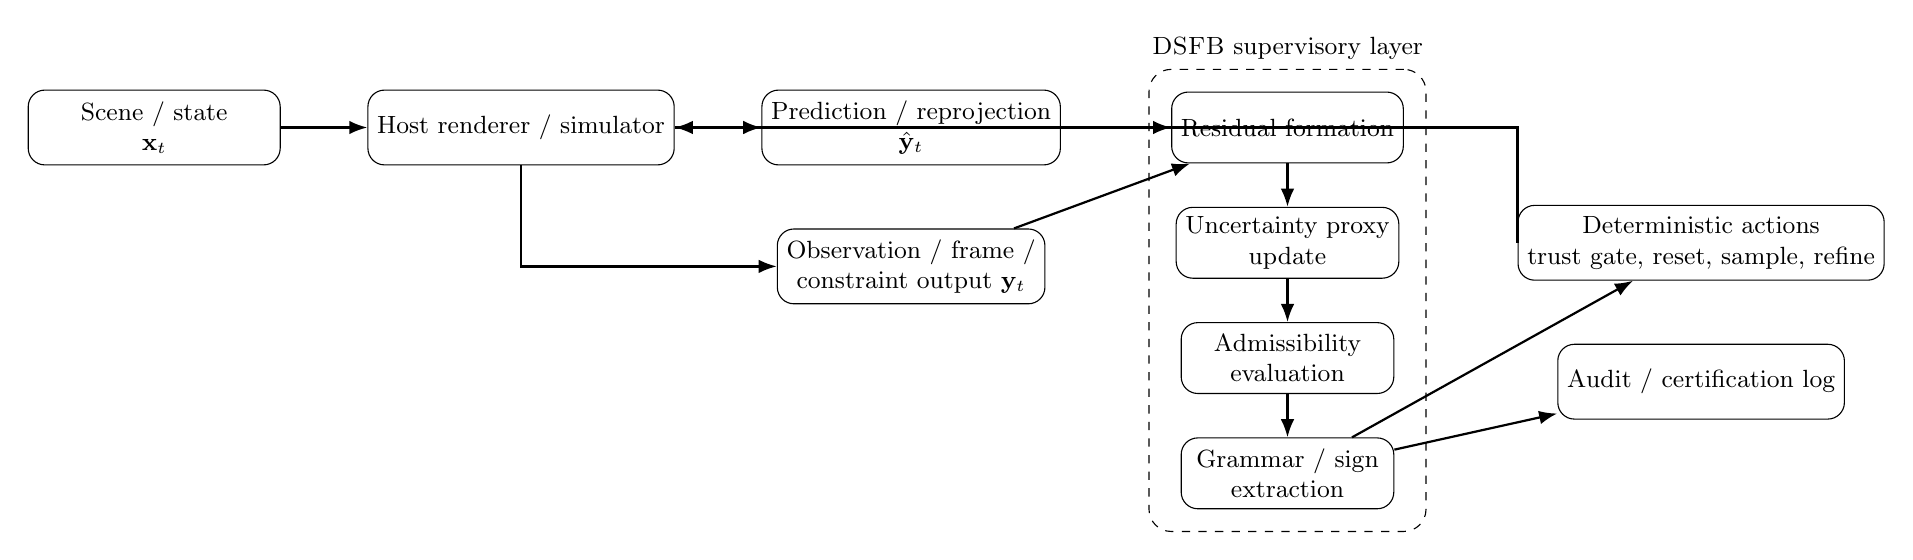
\begin{tikzpicture}[
font=\small,
node distance=0.8cm and 1.1cm,
box/.style={draw, rounded corners=6pt, minimum width=3.2cm, minimum height=0.95cm, align=center},
smallbox/.style={draw, rounded corners=6pt, minimum width=2.7cm, minimum height=0.9cm, align=center},
arrow/.style={-{Latex[length=2.3mm]}, thick}
]
\node[box] (scene) {Scene / state\\$\state_t$};
\node[box, right=of scene] (host) {Host renderer / simulator};
\node[box, right=of host] (pred) {Prediction / reprojection\\$\pred_t$};
\node[box, below=of pred] (obs) {Observation / frame /\\constraint output $\obs_t$};
\node[smallbox, right=1.4cm of pred] (res) {Residual formation};
\node[smallbox, below=0.55cm of res] (unc) {Uncertainty proxy\\update};
\node[smallbox, below=0.55cm of unc] (adm) {Admissibility\\evaluation};
\node[smallbox, below=0.55cm of adm] (gram) {Grammar / sign\\extraction};
\node[box, right=1.5cm of unc] (act) {Deterministic actions\\trust gate, reset, sample, refine};
\node[box, below=of act] (log) {Audit / certification log};

\draw[arrow] (scene) -- (host);
\draw[arrow] (host) -- (pred);
\draw[arrow] (host) |- (obs);
\draw[arrow] (pred) -- (res);
\draw[arrow] (obs) -- (res);
\draw[arrow] (res) -- (unc);
\draw[arrow] (unc) -- (adm);
\draw[arrow] (adm) -- (gram);
\draw[arrow] (gram) -- (act);
\draw[arrow] (gram) -- (log);
\draw[arrow] (act.west) |- (host.east);

\node[draw, dashed, rounded corners=8pt, fit=(res)(unc)(adm)(gram), inner sep=8pt, label=above:{\dsfb\ supervisory layer}] {};
\end{tikzpicture}
}
\caption{A host-attached view of \dsfb\ in a graphics or simulation pipeline. The host stack remains in place; \dsfb\ forms residuals, updates uncertainty semantics, evaluates admissibility, extracts structural signs, issues deterministic actions, and records replayable evidence.}
\label{fig:architecture}
\end{figure}

\subsection{Illustrative meta-residual excursion}
\begin{figure}[H]
\centering
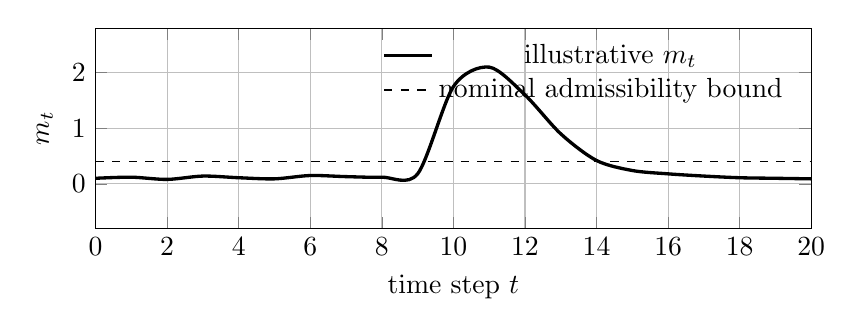
\begin{tikzpicture}
\begin{axis}[
    width=0.88\textwidth,
    height=0.34\textwidth,
    xlabel={time step $t$},
    ylabel={$\metares_t$},
    ymin=-0.8, ymax=2.8,
    xmin=0, xmax=20,
    grid=both,
    legend style={at={(0.98,0.98)},anchor=north east,draw=none,fill=none}
]
\addplot[smooth,very thick] coordinates {
(0,0.10) (1,0.12) (2,0.08) (3,0.14) (4,0.11) (5,0.09) (6,0.15) (7,0.13)
(8,0.12) (9,0.18) (10,1.75) (11,2.10) (12,1.60) (13,0.90) (14,0.42)
(15,0.24) (16,0.18) (17,0.14) (18,0.11) (19,0.10) (20,0.09)};
\addlegendentry{illustrative $\metares_t$}
\addplot[dashed] coordinates {(0,0.4) (20,0.4)};
\addlegendentry{nominal admissibility bound}
\end{axis}
\end{tikzpicture}
\caption{Illustrative meta-residual behavior during a regime shift. A nominally stable estimator remains within a bounded admissibility region until a sudden event causes a sharp excursion, followed by gradual re-equilibration.}
\label{fig:metaresidual}
\end{figure}

\subsection{Illustrative anisotropic covariance growth}
\begin{figure}[H]
\centering
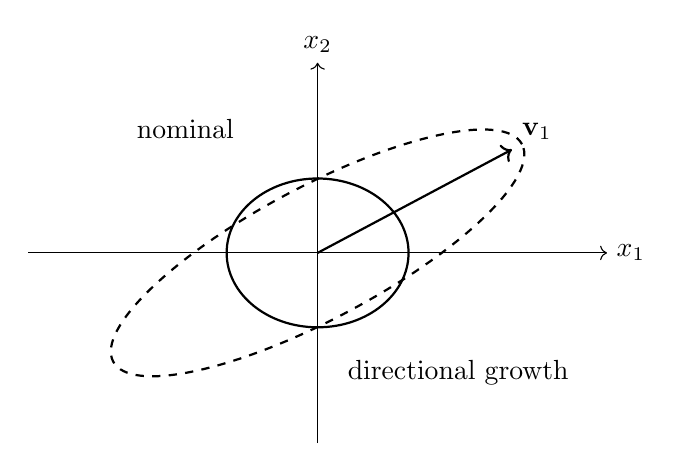
\begin{tikzpicture}[scale=1.05]
    \draw[->] (-3.5,0) -- (3.5,0) node[right] {$x_1$};
    \draw[->] (0,-2.3) -- (0,2.3) node[above] {$x_2$};
    \draw[thick] (0,0) ellipse (1.1 and 0.9);
    \draw[thick,dashed,rotate around={28:(0,0)}] (0,0) ellipse (2.8 and 0.8);
    \draw[->,thick] (0,0) -- (2.35,1.25) node[above right] {$\mathbf{v}_1$};
    \node at (-1.6,1.5) {nominal};
    \node at (1.7,-1.45) {directional growth};
\end{tikzpicture}
\caption{Illustrative covariance geometry. The dashed ellipse represents anisotropic uncertainty expansion, with principal direction $\mathbf{v}_1$ indicating the dominant unresolved mode.}
\label{fig:anisotropy}
\end{figure}

\subsection{Illustrative admissibility phase map}
\begin{figure}[H]
\centering
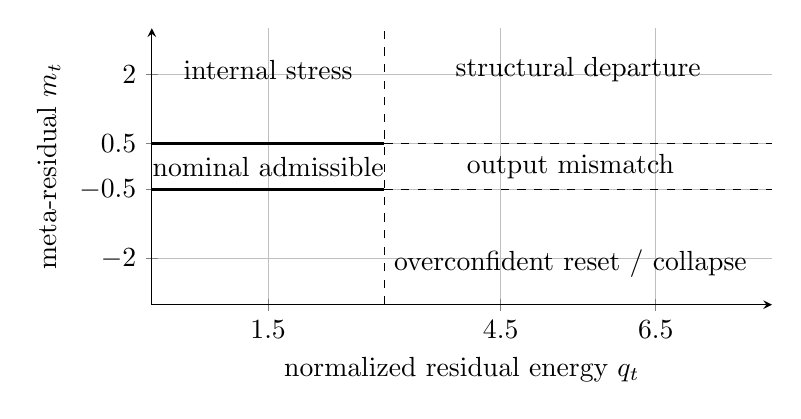
\begin{tikzpicture}
\begin{axis}[
    width=0.78\textwidth,
    height=0.42\textwidth,
    xlabel={normalized residual energy $q_t$},
    ylabel={meta-residual $\metares_t$},
    xmin=0, xmax=8,
    ymin=-3, ymax=3,
    axis lines=left,
    xtick={1.5,4.5,6.5},
    ytick={-2,-0.5,0.5,2},
    grid=both
]
\addplot[domain=0:3,samples=2,very thick] {0.5};
\addplot[domain=0:3,samples=2,very thick] {-0.5};
\addplot[domain=3:8,samples=2,dashed] {0.5};
\addplot[domain=3:8,samples=2,dashed] {-0.5};
\addplot[dashed] coordinates {(3,-3) (3,3)};
\node at (axis cs:1.5,0) {nominal admissible};
\node at (axis cs:5.4,0) {output mismatch};
\node at (axis cs:1.5,2.1) {internal stress};
\node at (axis cs:5.5,2.1) {structural departure};
\node at (axis cs:5.4,-2.1) {overconfident reset / collapse};
\end{axis}
\end{tikzpicture}
\caption{Conceptual phase map illustrating why \dsfb\ uses more than a scalar residual threshold. Moderate residual energy with large positive meta-residual indicates estimator stress, while simultaneous residual and meta-residual excursions suggest a structural regime departure.}
\label{fig:phase_map}
\end{figure}

% =========================================================
\section{Use Cases and Prior-Art-Relevant Application Surfaces}

For licensing and SBIR-oriented positioning, it is useful to state where the framework can be applied without overcommitting to a single implementation path.

\subsection{Application surfaces}
\begin{table}[H]
\centering
\caption{Representative application surfaces for a \dsfb\ graphics stack.}
\label{tab:applications}
\begin{tabularx}{\textwidth}{>{\raggedright\arraybackslash}p{0.22\textwidth} >{\raggedright\arraybackslash}p{0.24\textwidth} >{\raggedright\arraybackslash}X}
\toprule
\textbf{Area} & \textbf{Primary residual source} & \textbf{Potential \dsfb\ role} \\
\midrule
Temporal rendering & reprojection mismatch, history disagreement & detect disocclusion, stale history, motion inconsistency, trust-gated accumulation \\
Path tracing & sample-to-prediction mismatch, transport instability & adaptive sampling, structural stopping rules, difficult-light-path detection \\
Neural rendering & feature prediction residuals, latent drift & regime diagnostics, uncertainty supervision, out-of-regime warnings \\
Inverse graphics & render-to-observation mismatch & identifiability diagnostics, trust gating, model-structure mismatch classification \\
Physical simulation & constraint residuals, energy imbalance, contact mismatch & instability monitoring, step-size supervision, regime-aware solver intervention \\
Graphics certification / QA & aggregate residual histories & evidence logging, acceptance envelopes, replayable anomaly signatures \\
\bottomrule
\end{tabularx}
\end{table}

\subsection{Evidence logging and certification-oriented workflows}
A notable commercialization advantage of the framework is that it converts internal graphics signals into replayable evidence. A \dsfb\ log can include time-stamped residual excursions, regime descriptors, extracted signs, intervention traces, uncertainty-growth summaries, and post-intervention outcomes. This matters for quality assurance, simulation trust monitoring, digital twins, and defense-oriented visualization because it supports auditability rather than mere black-box confidence. The logging channel is therefore not an afterthought; it is part of the intended application surface.

\subsection{Why this matters for future transition work}
A later commercial or SBIR effort can specialize this framework to a particular market surface: real-time rendering quality assurance, simulation trust monitoring, deterministic adaptive sampling, neural rendering diagnostics, or integrated graphics certification tooling. The present paper is broad enough to establish the conceptual territory, yet specific enough to identify implementation hooks and patent-adjacent language without exaggeration.

% =========================================================
\section{Evaluation Protocol for Future Empirical Validation}

The present paper is theoretical and architectural rather than empirical. Nevertheless, a serious transition path requires an explicit validation protocol. This section states what a disciplined evaluation program should measure.

\subsection{Temporal accumulation and TAA evaluation}
A temporal-accumulation benchmark should include events such as disocclusion, motion-vector failure, view-dependent specular flicker, and stale-history contamination. Primary metrics should include detection latency, false positive rate, region-level classification accuracy, post-intervention ghosting reduction, and quality-cost tradeoff. The purpose is not merely to show that residuals exist, but to test whether structural signs trigger useful interventions earlier or more precisely than scalar thresholds alone.

\subsection{Path tracing and adaptive sampling evaluation}
A Monte Carlo benchmark should include difficult caustics, glossy transport, underresolved indirect light, and estimator stagnation under fixed sampling budgets. Relevant metrics include error reduction at fixed sample budget, budget reduction at fixed target error, structural detection accuracy for difficult transport, and the degree to which early anisotropic-growth signals correlate with eventual image error.

\subsection{Simulation monitoring evaluation}
A simulation benchmark should include contact inconsistency, near-instability, energy imbalance, and divergence onset. Primary metrics include early-warning horizon, false alarms under benign stiff dynamics, intervention success rate, and computational overhead. In this context the value of \dsfb\ is not just detection, but structured supervision of solver trust and intervention timing.

\begin{table}[H]
\centering
\caption{Evaluation surfaces and example metrics for future validation.}
\label{tab:evaluation}
\begin{tabularx}{\textwidth}{>{\raggedright\arraybackslash}p{0.18\textwidth} >{\raggedright\arraybackslash}p{0.19\textwidth} >{\raggedright\arraybackslash}p{0.16\textwidth} >{\raggedright\arraybackslash}p{0.19\textwidth} >{\raggedright\arraybackslash}X}
\toprule
\textbf{Domain} & \textbf{Event type} & \textbf{\dsfb\ output} & \textbf{Primary metric} & \textbf{Secondary metric} \\
\midrule
TAA & disocclusion & $\sigma_{\mathrm{occ}}$ & detection latency & false positives \\
TAA & stale history & $\sigma_{\mathrm{hist}}$ & ghosting reduction & temporal stability \\
Path tracing & difficult transport & anisotropic growth / sign label & budget efficiency & residual--error correlation \\
Inverse graphics & ambiguity / drift & $\sigma_{\mathrm{amb}}$, $\metares_t$ & trust-gated convergence quality & misclassification rate \\
Simulation & instability onset & $\sigma_{\mathrm{sim}}$, $\metares_t$ & early-warning horizon & intervention overhead \\
\bottomrule
\end{tabularx}
\end{table}

\subsection{Baselines and comparative posture}
Future validation should compare \dsfb\ against relevant baselines such as scalar variance thresholds, heuristic history rejection, standard solver residual thresholds, confidence-only gating, and other host-native diagnostics. The purpose of such comparison is not to denigrate existing methods. On the contrary, it is to determine where structural residual interpretation adds value, where it does not, and how it interacts with established practices.

% =========================================================
\section{Relation to Classical Estimation, Change Detection, and Inverse Problems}

The framework benefits from explicit positioning relative to existing estimation theory. Doing so improves rigor and avoids accidental novelty inflation.

\subsection{Relation to innovation-based consistency testing}
The statistic
\begin{equation}
    q_t = \resid_t^\top \innov_t^{-1}\resid_t
\end{equation}
is familiar from innovation-based consistency testing in state estimation. \dsfb\ does not replace such testing. Rather, it extends scalar consistency checking by adding regime-relative admissibility, structural grammar, and sign extraction over histories. In other words, innovation testing remains one ingredient inside a broader structural supervisory framework.

\subsection{Relation to classical change detection}
Classical change detection methods seek evidence for distribution or regime change from time-series observations. \dsfb\ is compatible with that tradition but contributes a different emphasis: it organizes residual histories into structured classes before or alongside thresholding. In this sense the framework can supply structured features to sequential detectors without claiming to supersede them.

\subsection{Relation to inverse problems}
Inverse problems already rely on mismatch structure to infer latent causes. \dsfb\ adds an explicit regime-aware grammar to that mismatch structure. This is particularly useful when identifiability varies by scene, view, lighting, or regularization regime. The goal is not to turn inverse problems into symbolic logic, but to introduce a deterministic supervisory language for recurring residual organizations.

\subsection{Relation to robust estimation}
The framework is not itself a robust filter, $H_\infty$ estimator, or complete uncertainty calculus. It is more appropriately viewed as a supervisory layer that can modify trust, gating, intervention, or logging policy when residual structure suggests regime departure. This distinction matters because it prevents conceptual overreach while clarifying where the method attaches to classical estimation practice.

% =========================================================
\section{Transition Path and Phase-I-Oriented Demonstration Surfaces}

A prior-art paper intended to support later licensing and SBIR transition should identify concrete first demonstrations rather than leaving all engineering choices implicit.

\subsection{Candidate demonstration surfaces}
Three initial demonstration surfaces appear particularly practical.

\paragraph{Demo A: \dsfb--TAA trust gate.}
Objective: detect disocclusion, stale history, and motion inconsistency early enough to reduce ghosting and mistrust accumulation. Expected deliverables include a prototype supervisory module, benchmark scenes, detection metrics, an overhead profile, and replayable anomaly signatures.

\paragraph{Demo B: \dsfb\ adaptive sampler.}
Objective: use anisotropic residual growth and structural labels to route additional samples toward unresolved regions in path tracing. Expected deliverables include a path-tracer integration, stopping-rule comparisons, budget--error curves, and curated difficult-transport scenes.

\paragraph{Demo C: \dsfb\ simulation monitor.}
Objective: use residual structure and meta-residual growth to detect contact or constraint stress before visible instability. Expected deliverables include a solver wrapper, early-warning metrics, intervention policies, and certification-oriented logs.

\begin{table}[H]
\centering
\caption{Illustrative prioritization of early transition surfaces.}
\label{tab:phase1}
\begin{tabularx}{\textwidth}{>{\centering\arraybackslash}p{0.09\textwidth} >{\raggedright\arraybackslash}p{0.25\textwidth} >{\raggedright\arraybackslash}X}
\toprule
\textbf{Priority} & \textbf{Demonstration} & \textbf{Reason for ordering} \\
\midrule
1 & \dsfb--TAA trust gate & lowest integration risk, immediately visible qualitative effects, strong metrics for detection latency and ghosting reduction \\
2 & \dsfb\ adaptive sampler & clear efficiency story, attractive for licensing, strong connection to anisotropic-growth thesis \\
3 & \dsfb\ simulation monitor & high-value supervisory application but broader integration complexity across host simulators \\
\bottomrule
\end{tabularx}
\end{table}

\subsection{Why this ordering is technically sensible}
The TAA case is the natural first demonstration because it is easy to instrument, visually legible, rich in residual structure, and strongly connected to trust gating. The adaptive-sampling case follows naturally because it exploits the directional-growth thesis. Simulation monitoring remains highly promising, but the surrounding host complexity is typically larger.
%############################
% 21. DISCUSSION
%############################

\section{Discussion}
\label{sec:discussion}

This section reflects on the broader implications of the DSFB framework in computer graphics, clarifies its role relative to existing methodologies, and identifies conceptual boundaries. The aim is to position the contribution accurately: as a supervisory and interpretive layer that augments estimation and reconstruction pipelines through structured residual analysis.

%----------------------------
% Position within graphics systems
%----------------------------

\subsection{Position within graphics systems}

DSFB operates as a \emph{supervisory layer} rather than a primary estimator. It does not replace rendering, reconstruction, or neural inference modules. Instead, it observes their behavior through residuals and derived diagnostics, and regulates their usage through trust, intervention, and routing. In the current paper, the only verified empirical wedge is trust-regulated temporal reuse on the frozen five-capture Unreal-native sequence.

The strongest current finding is therefore hybrid rather than standalone. The fixed DSFB+strong-heuristic method is the best current Demo A result, while pure DSFB remains heuristic-favorable on all five captures. DSFB alone does not outperform strong heuristic baselines in the current evaluation.

This separation has several implications:

\begin{itemize}[leftmargin=1.5em]
    \item it can be integrated into diverse pipelines without requiring architectural redesign,
    \item it remains compatible with both classical and neural methods,
    \item it provides a unifying control layer across heterogeneous components,
    \item but its current validated claim is much narrower than the full conceptual surface of the manuscript.
\end{itemize}

%----------------------------
% Relationship to heuristic confidence measures
%----------------------------

\subsection{Relationship to heuristic confidence measures}

Many graphics systems employ confidence heuristics (e.g., based on motion magnitude or variance). DSFB differs in that:

\begin{itemize}[leftmargin=1.5em]
    \item residuals are interpreted relative to regime-dependent admissibility,
    \item multiple diagnostics (integrity, anisotropy, envelopes) are combined,
    \item trust evolves over time with memory and suppression–recovery dynamics,
    \item decisions are conditioned on structural grammar rather than scalar thresholds alone.
\end{itemize}

These distinctions provide a more structured and interpretable basis for supervisory control.

%----------------------------
% Structural interpretation vs. magnitude-based reasoning
%----------------------------

\subsection{Structural interpretation vs. magnitude-based reasoning}

A central theme of this work is that magnitude alone is insufficient for reliable supervision. Small residuals may be structurally inconsistent, while large residuals may be admissible under certain regimes.

By introducing admissibility envelopes and grammar-based interpretation, DSFB emphasizes \emph{structural compatibility} over raw magnitude. This perspective aligns with the detectability results in Section~\ref{sec:detectability} and informs intervention and routing decisions throughout the framework.

%----------------------------
% Interaction with neural methods
%----------------------------

\subsection{Interaction with neural methods}

Neural components introduce flexibility but also variability and potential instability. DSFB provides a mechanism for monitoring and regulating these modules without constraining their internal design.

In particular:
\begin{itemize}[leftmargin=1.5em]
    \item neural outputs are evaluated through residual consistency and proxy evolution,
    \item integrity signals capture latent instability,
    \item trust modulation enables adaptive blending with classical estimates.
\end{itemize}

This allows neural methods to be used more robustly in dynamic and out-of-distribution conditions.

%----------------------------
% Interpretability and diagnostics
%----------------------------

\subsection{Interpretability and diagnostics}

A notable feature of DSFB is the interpretability of its internal signals:

\begin{itemize}[leftmargin=1.5em]
    \item residuals provide direct discrepancy measures,
    \item proxies encode uncertainty structure,
    \item grammar labels categorize structural conditions,
    \item trust summarizes supervisory confidence.
\end{itemize}

These signals can be visualized and analyzed, supporting debugging, tuning, and system understanding.

%----------------------------
% Trade-offs
%----------------------------

\subsection{Trade-offs}

The introduction of a supervisory layer involves trade-offs:

\begin{itemize}[leftmargin=1.5em]
    \item additional computation for diagnostics,
    \item need for calibration of thresholds and gains,
    \item increased system complexity,
    \item potential sensitivity to proxy and residual design.
\end{itemize}

These trade-offs are balanced by improved robustness, interpretability, and adaptability.

%----------------------------
% Scope and limitations
%----------------------------

\subsection{Scope and limitations}

The most important limitations are empirical and specific to the current benchmark. DSFB alone does not outperform the strong heuristic baseline in the current evaluation; the best current story is the fixed DSFB+strong-heuristic hybrid, not DSFB in isolation. The ROI mask covers 50.60\% $\pm$ 18.61\% of the frame, so ROI MAE is closer to a broad structural error measure than to a sparse artifact score. Demo B is positive but moderate, and it remains an allocation proxy rather than a renderer-integrated sampling result. The GPU numbers are imported-buffer compute-path timings on an RTX 4080 SUPER / Vulkan path, not full in-engine production timings. The evidence itself remains narrow: five real captures from one ordered shot, using exported \texttt{reference\_color} rather than path-traced ground truth.

The framework is intended to:

\begin{itemize}[leftmargin=1.5em]
    \item detect and respond to structural inconsistency,
    \item regulate existing estimation processes,
    \item improve stability under regime variation.
\end{itemize}

It is not intended to:

\begin{itemize}[leftmargin=1.5em]
    \item replace underlying rendering or learning algorithms,
    \item guarantee optimal reconstruction,
    \item eliminate all artifacts or errors.
\end{itemize}

Performance depends on the quality of inputs, proxy construction, and calibration.

%----------------------------
% Broader implications
%----------------------------

\subsection{Broader implications}

The DSFB perspective suggests a general pattern for complex systems:

\begin{itemize}[leftmargin=1.5em]
    \item interpret residuals as structured signals,
    \item define admissibility relative to context,
    \item track internal consistency through proxies,
    \item regulate system behavior through trust and intervention.
\end{itemize}

While this paper focuses on computer graphics, similar ideas may be applicable in other domains involving dynamic estimation and reconstruction. In the present manuscript, however, that broader reach remains conceptual rather than empirically demonstrated.

%----------------------------
% Summary
%----------------------------

\subsection{Summary}

DSFB provides a structured supervisory layer that complements existing graphics pipelines. In the current evidence base, the main empirical statement is narrow: DSFB improves strong temporal heuristics via structural supervision on the frozen Unreal-native temporal-reuse benchmark. The next section sharpens the remaining limitations and future-work boundary.


%----------------------------
%----------------------------
% Operator Evaluation and Licensing Rationale (Phase I Execution)
%----------------------------

\section{Operator Evaluation and Licensing Rationale (Phase I Execution)}

\subsection{Objective}
This work introduces DSFB as a deterministic supervisory layer for temporal rendering pipelines. The objective for an operator is not immediate production replacement, but low-risk internal evaluation of an additional observability and control axis over existing estimators.

\subsection{Overview}
DSFB (Deterministic Structural Functional Blocks) is a read-only supervisory layer designed to operate alongside existing temporal rendering systems. It does not replace, modify, or interfere with current pipelines (e.g., temporal anti-aliasing, reconstruction, or upscaling). Instead, it observes already-available signals (e.g., current frame, reprojected history, motion vectors) and produces deterministic supervisory outputs derived from residual structure.

\subsection{Acquisition Model}
DSFB is structured for acquisition as a licensing-based supervisory technology. The reference implementation and accompanying prior-art corpus define the architecture, operational contract, and expected behavior. Full integration, scaling, and production validation are intended to be executed internally by the operator.

Due to export-control constraints, the originating author participates only in a non-operational advisory capacity. All implementation, validation, and deployment work is designed to be performed independently by the licensing entity.

\subsection{Integration Model}
DSFB can be integrated as a side-channel compute pass operating on exported buffers. No modification to core rendering logic is required. If disabled, system behavior remains unchanged. This ensures zero regression risk and allows incremental evaluation within existing pipelines.

\subsection{Minimal Integration Path}
A minimal evaluation requires only existing pipeline signals:
\begin{itemize}
    \item Current frame color buffer
    \item Reprojected history buffer
    \item Motion vectors or equivalent proxy
\end{itemize}

DSFB can be implemented as an auxiliary compute or post-process stage that:
\begin{enumerate}
    \item Computes residuals between current and predicted signals
    \item Extracts drift and slew structure over time
    \item Produces a trust field and optional diagnostic masks
\end{enumerate}

No modification to upstream rendering, temporal accumulation, or reconstruction systems is required.


\subsection{Compute Characteristics and Deployment Profiles}

The reference implementation evaluates supervisory signals using full residual structure and neighborhood interactions. This configuration is intended as a diagnostic and validation profile.

For deployment, reduced variants can be constructed, for example:
\begin{itemize}
    \item diagonal proxy evaluation (avoiding full matrix operations)
    \item reduced neighborhood interaction
\end{itemize}

These reduced forms retain core supervisory structure while lowering computational cost. The reference implementation should therefore be interpreted as a full evaluation configuration rather than a production-optimized path.

No claim is made that the reported execution cost reflects optimized inline deployment or full engine integration.



\subsection{Compute Characteristics and Deployment Profiles}

The reference implementation evaluates supervisory signals using full residual structure and neighborhood interactions. This configuration is intended as a diagnostic and validation profile.

For deployment, reduced variants can be constructed, for example:
\begin{itemize}
    \item diagonal proxy evaluation (avoiding full matrix operations)
    \item reduced neighborhood interaction
\end{itemize}

These reduced forms retain core supervisory structure while lowering computational cost. The reference implementation should therefore be interpreted as a full evaluation configuration rather than a production-optimized path.

No claim is made that the reported execution cost reflects optimized inline deployment.

\paragraph{Deployment Tiers}
For clarity, two representative usage tiers can be distinguished:
\begin{itemize}
    \item \textbf{Reference Tier:} full supervisory evaluation used for analysis, validation, and signal inspection
    \item \textbf{Inline Tier:} reduced proxy-based evaluation intended for integration under strict runtime constraints
\end{itemize}

The present work evaluates the reference configuration; optimized inline variants are left to implementation-specific integration.


\subsection{Operational Contract}
The evaluation model is governed by a strict non-interference contract:
\begin{itemize}
    \item DSFB is read-only with respect to host buffers
    \item DSFB outputs are auxiliary and not consumed by default
    \item DSFB can be enabled or disabled with zero impact on baseline behavior
\end{itemize}

This ensures that evaluation carries no regression risk to the host system.

% ============================
% Minimal Inline Deployment (Fast-Path Proxy)
% ============================

\subsection{Minimal Inline Deployment (Fast-Path Proxy)}

In addition to the reference supervisory evaluation, a reduced inline configuration is defined to assess deployment feasibility under real-time constraints. This configuration does not evaluate the full DSFB structure, but instead implements a per-pixel proxy derived from residual evolution.

\paragraph{Scope}

The inline configuration is constructed under the following constraints:
\begin{itemize}
    \item single-pass per-pixel computation
    \item no dynamic allocation
    \item no matrix operations or eigendecomposition
    \item local temporal structure only (first- and second-order differences)
\end{itemize}

The intent is not to reproduce the full supervisory system, but to evaluate whether a reduced proxy preserves core signal behavior at significantly lower computational cost.

\paragraph{Per-Pixel Quantities}

For each pixel, the following quantities are computed:
\begin{itemize}
    \item residual magnitude $r_t = \lVert C_t - H_t \rVert_1$
    \item drift $d_t = r_t - r_{t-1}$
    \item slew $s_t = d_t - d_{t-1}$
\end{itemize}

A scalar proxy is then defined as:
\[
u_t = |d_t| + \lambda |s_t|
\]

where $\lambda$ is a fixed weighting parameter.

\paragraph{Trust Proxy}

A trust value is derived from the proxy:
\[
T_t = \mathrm{saturate}(1 - k \cdot u_t)
\]

where $k$ is a scaling constant. This mapping is linear and bounded, and avoids nonlinear functions such as sigmoid evaluation.

\paragraph{Optional Local Aggregation}

A local aggregation over a $3\times3$ neighborhood may be applied:
\[
u'_t = \mathrm{mean}_{N(3\times3)}(u_t)
\]

with trust evaluated using $u'_t$ instead of $u_t$. This operation is optional and introduces limited additional cost.

\paragraph{Implementation Characteristics}

The inline configuration uses:
\begin{itemize}
    \item a single compute pass
    \item per-pixel state consisting of residual and drift history (two scalar buffers)
    \item one output buffer for trust
\end{itemize}

No claim is made that this configuration captures all supervisory structure present in the full system. It is intended as a reduced proxy suitable for integration and performance evaluation.

\paragraph{Execution Time}

Execution time is measured on the same hardware as the reference implementation using wgpu (Vulkan backend) on an NVIDIA GeForce RTX 4080 SUPER. Timings are CPU-side wall-clock measurements of dispatch and synchronisation (3 warmup runs, mean of 10 measured runs). Representative results are reported in Table~\ref{tab:dsfb_fastpath}.

\begin{table}[H]
\centering
\caption{Minimal DSFB fast-path execution time (RTX 4080 SUPER, Vulkan, wgpu)}
\label{tab:dsfb_fastpath}
\begin{tabular}{l l}
\hline
Resolution & Time (ms) \\
\hline
1920$\times$1080 & 1.44 \\
3840$\times$2160 & 5.74 \\
\hline
\end{tabular}
\end{table}

These measurements reflect the reduced proxy configuration only and should not be interpreted as the cost of the full supervisory system.

\paragraph{Interpretation}

The inline configuration demonstrates that supervisory signals derived from residual evolution can be evaluated using a constrained per-pixel formulation. This supports the feasibility of integrating DSFB-derived signals into existing pipelines under strict runtime budgets, while maintaining separation from upstream rendering logic.



\subsection{What DSFB Provides}
DSFB computes structured signals from residuals, including magnitude, persistence (drift), and temporal change (slew). These signals provide a deterministic and reproducible description of temporal behavior that is not explicitly represented in existing confidence or variance metrics.

The primary output is a supervisory signal (e.g., trust or admissibility) that can be used optionally to:
\begin{itemize}
    \item analyze temporal stability and failure modes
    \item support debugging and tuning of existing heuristics
    \item inform selective gating or modulation strategies
\end{itemize}

\subsection{What DSFB Does Not Do}
\begin{itemize}
    \item does not perform reconstruction, upscaling, or denoising
    \item does not replace existing methods (e.g., DLSS, FSR, XeSS)
    \item does not require training, datasets, or model fitting
    \item does not introduce feedback into the rendering pipeline unless explicitly integrated
\end{itemize}

\subsection{Risk Profile}
\begin{itemize}
    \item \textbf{Non-intrusive:} operates in read-only mode
    \item \textbf{Deterministic:} identical inputs produce identical outputs
    \item \textbf{Isolated:} can be enabled or disabled without affecting system behavior
    \item \textbf{Incremental:} can be evaluated without full pipeline integration
\end{itemize}

\subsection{Evaluation Scope (Phase I)}
A Phase I effort is expected to focus on:
\begin{itemize}
    \item Integration as an external supervisory pass
    \item Execution across representative scenes and motion regimes
    \item Comparison against existing temporal diagnostics or heuristics
    \item Assessment of DSFB signals relative to known artifact occurrences
\end{itemize}

Key evaluation questions include:
\begin{itemize}
    \item Does DSFB expose instability earlier than existing metrics?
    \item Does it provide additional diagnostic clarity for known failure modes?
    \item Is the computational overhead acceptable within target constraints?
\end{itemize}

\subsection{Expected Outcomes}
This work does not claim improvements in visual quality or performance. The expected outcome of evaluation is increased observability of temporal behavior and identification of conditions under which DSFB signals correlate with instability.

If effective, DSFB may provide:
\begin{itemize}
    \item A structured supervisory signal over temporal reuse and reconstruction
    \item Improved visibility into failure modes such as ghosting, disocclusion, and instability
    \item A signal that can be optionally integrated into existing heuristics or control policies
\end{itemize}

If ineffective, DSFB can be removed without any impact on system performance or output.

\subsection{Why This Is Low Risk to Evaluate}
\begin{itemize}
    \item requires no architectural changes to existing systems
    \item does not compete with or replace current methods
    \item produces additional signals without altering outputs
    \item can be evaluated in isolation using existing data flows
\end{itemize}

\subsection{Rationale for Licensing}
DSFB is not positioned as a standalone rendering method, but as a complementary supervisory framework grounded in a broader prior-art corpus. While the minimal implementation is straightforward, the full structure—including residual grammar, admissibility envelopes, and trust field interpretation—represents a non-trivial design space.

Licensing provides access to:
\begin{itemize}
    \item A coherent and internally consistent supervisory architecture
    \item A validated reference implementation with reproducible artifacts
    \item A formalized framework that avoids re-derivation and iteration overhead
\end{itemize}

\subsection{Summary}
DSFB offers a low-risk, non-intrusive path to augment existing rendering pipelines with additional structure and observability. Its design ensures that evaluation is safe, bounded, and fully under operator control, while its potential value lies in improved interpretability and diagnostic capability for temporal systems.

%----------------------------
% Limitations and future work (LEGENDARY VERSION)
%----------------------------

\section{Limitations and future work}

While the DSFB framework provides a structured supervisory layer for graphics pipelines, its effectiveness is bounded by several fundamental and practical limitations. These are not peripheral considerations; they define the operational envelope of the method and inform both deployment and future research.

\vspace{0.5em}
\noindent
\textbf{Current empirical boundaries.}

Before broader theoretical limitations, the present manuscript makes five benchmark-specific boundaries explicit:
\begin{itemize}[leftmargin=1.5em]
    \item DSFB alone does not outperform the strong heuristic baseline in the current evaluation; the best current result is the fixed DSFB+strong-heuristic hybrid.
    \item The ROI definition captures approximately 50\% of the frame, with measured coverage 50.60\% $\pm$ 18.61\%, so ROI MAE behaves more like a broad structural error metric than a sparse artifact score.
    \item Demo B is a budget-preserving allocation proxy rather than a renderer-integrated adaptive-budget benchmark.
    \item The reported 1.0391\,ms, 17.5886\,ms, and 67.7201\,ms timings are imported-buffer GPU scaling measurements on an RTX 4080 SUPER / Vulkan path, not final in-engine production timings.
    \item The canonical evaluation covers five real captures from one ordered shot and uses exported \texttt{reference\_color} rather than path-traced ground truth.
\end{itemize}

\vspace{0.5em}
\noindent
\textbf{Allowed and disallowed posture.}

The crate ships \texttt{docs/FAILURE\_MODES.md}, which records the official allowed/not-allowed posture for describing the current evidence. That document is the authoritative source for claim boundaries and should be consulted before any public communication about the results. The key entries are: \emph{allowed} --- ``DSFB improves strong temporal heuristics via structural supervision (fixed hybrid result)'', ``trust is a useful supervisory signal in the current sequence''; \emph{not allowed} --- ``DSFB replaces TAA or any existing temporal method'', ``DSFB outperforms strong heuristics on its own'', ``the current evidence generalizes across scenes or shots''. Any claim that is not explicitly permitted in \texttt{docs/FAILURE\_MODES.md} should be treated as deferred pending additional evidence.\footnote{The posture table in \texttt{docs/FAILURE\_MODES.md} is part of the invariant set of this crate and is not modified by this revision.}

\vspace{0.5em}
\noindent
\textbf{1. Dependence on residual informativeness.}

The framework relies on residual signals as its primary observational channel. If the residual stack $\mathbf{r}_t(u)$ does not encode meaningful discrepancies between prediction and observation, DSFB cannot infer structural inconsistency.

\begin{itemize}[leftmargin=1.5em]
    \item If residuals are \emph{uninformative} (e.g., due to aggressive filtering, saturation, or cancellation), structural failure may remain undetected.
    \item If residuals are \emph{biased but consistent}, the system may interpret them as admissible under the current regime.
\end{itemize}

Thus, DSFB does not create information; it organizes and interprets it. The quality of supervision is bounded by the informativeness of the residual channels.

\vspace{0.5em}
\noindent
\textbf{2. Proxy fidelity and hidden-state observability.}

The uncertainty proxy $\Sigma_t(u)$ is a constructed object, not a directly observed quantity. Its ability to reflect latent instability depends on the chosen proxy formulation.

\begin{itemize}[leftmargin=1.5em]
    \item If proxy construction fails to capture relevant latent degrees of freedom, integrity signals may miss hidden failure modes.
    \item Different proxy designs may emphasize different aspects of uncertainty, leading to variation in sensitivity.
\end{itemize}

This introduces an observability limitation: DSFB can only detect instability that is expressed through the proxy representation.

\vspace{0.5em}
\noindent
\textbf{3. Regime specification and admissibility design.}

Admissibility is defined relative to a regime descriptor $\rho_t(u)$. Mis-specification of regimes or envelopes can lead to systematic errors:

\begin{itemize}[leftmargin=1.5em]
    \item overly permissive envelopes delay detection of structural failure,
    \item overly restrictive envelopes induce unnecessary intervention,
    \item incorrect regime classification leads to misinterpretation of residuals.
\end{itemize}

This reflects a broader limitation: DSFB requires a meaningful partitioning of operating conditions. It does not eliminate the need for domain knowledge; it formalizes its use.

\vspace{0.5em}
\noindent
\textbf{4. Calibration sensitivity and parameter coupling.}

The framework introduces parameters at multiple levels:

\begin{itemize}[leftmargin=1.5em]
    \item normalization scales,
    \item admissibility thresholds,
    \item trust aggregation weights,
    \item suppression and recovery gains.
\end{itemize}

These parameters are not independent. Coupling effects can arise:

\begin{itemize}[leftmargin=1.5em]
    \item tightening admissibility thresholds increases sensitivity of trust decay,
    \item aggressive suppression gains amplify noise in poorly filtered signals,
    \item routing policies interact with trust dynamics to affect stability.
\end{itemize}

As a result, calibration must be performed holistically rather than component-wise.

\vspace{0.5em}
\noindent
\textbf{5. Non-optimality and absence of global guarantees.}

DSFB is a supervisory framework, not an optimal estimator. It does not guarantee:

\begin{itemize}[leftmargin=1.5em]
    \item minimal reconstruction error,
    \item optimal allocation of compute,
    \item or globally optimal intervention decisions.
\end{itemize}

The detectability results (Section~\ref{sec:detectability}) ensure that persistent structural inconsistency leads to trust degradation, but they do not specify optimal detection delay or false-positive rates.

This distinction is intentional: the framework prioritizes interpretability and bounded behavior over optimality claims.

\vspace{0.5em}
\noindent
\textbf{6. Latency and delayed detectability.}

Detectability is finite-time, not instantaneous. In practice:

\begin{itemize}[leftmargin=1.5em]
    \item slowly accumulating errors may require multiple frames before trust degrades,
    \item intermittent violations may delay detection depending on anomaly memory parameters,
    \item rapid transient failures may not trigger intervention if they remain within admissibility bounds.
\end{itemize}

Thus, DSFB provides \emph{bounded detectability}, not zero-delay detection.

\vspace{0.5em}
\noindent
\textbf{7. Interaction with upstream and downstream systems.}

DSFB operates within a larger pipeline. Its behavior depends on interactions with:

\begin{itemize}[leftmargin=1.5em]
    \item temporal reuse mechanisms,
    \item neural modules,
    \item sampling and shading systems.
\end{itemize}

Feedback loops may arise:

\begin{itemize}[leftmargin=1.5em]
    \item aggressive intervention may reduce residual magnitude, altering future diagnostics,
    \item routing decisions may change noise characteristics,
    \item neural fallback may introduce different residual structures.
\end{itemize}

These interactions can produce emergent behaviors that are not fully captured by isolated analysis.

\vspace{0.5em}
\noindent
\textbf{8. Computational and systems overhead.}

Although designed to be lightweight, DSFB introduces additional computation:

\begin{itemize}[leftmargin=1.5em]
    \item residual processing and normalization,
    \item proxy updates,
    \item trust and routing evaluation,
    \item logging and diagnostics.
\end{itemize}

In real-time systems, this overhead must be carefully managed and may constrain deployment on lower-power hardware.

\vspace{0.5em}
\noindent
\textbf{9. No direct perceptual guarantee.}

The trust field $T_t(u)$ encodes structural confidence, not perceptual quality. It is possible for:

\begin{itemize}[leftmargin=1.5em]
    \item low-trust regions to appear visually acceptable,
    \item high-trust regions to contain perceptually noticeable artifacts.
\end{itemize}

Perceptual alignment depends on the relationship between residual structure and human visual sensitivity, which is not explicitly modeled in the current framework.

\vspace{0.5em}
\noindent
\textbf{10. Scope of validation.}

The empirical evaluation (Section~\ref{sec:evaluation}) is necessarily limited:

\begin{itemize}[leftmargin=1.5em]
    \item not all scene types, materials, or motion regimes are exhaustively covered,
    \item results depend on implementation details and datasets,
    \item cross-engine generalization requires further validation.
\end{itemize}

Therefore, conclusions should be interpreted within the scope of the evaluated scenarios.

\vspace{0.5em}
\noindent
\textbf{Future work.}

Several directions follow naturally from these limitations:

\begin{itemize}[leftmargin=1.5em]
    \item data-driven or adaptive calibration of admissibility envelopes,
    \item improved proxy constructions capturing richer latent structure,
    \item integration with perceptual models for trust alignment,
    \item hardware-aware optimization of diagnostic computation,
    \item formal analysis of coupled system dynamics under DSFB supervision,
    \item integration of CUSUM or EWMA change-detection statistics as additional grammar features (see Section~\ref{sec:classical}),
    \item extension of the grammar classifier to the $\sigma_{\mathrm{unstable}}$ and $\sigma_{\mathrm{spec}}$ labels via multi-frame persistence tracking.
\end{itemize}

\paragraph{Failure mode posture.}
The crate ships \texttt{docs/FAILURE\_MODES.md}, which maintains a machine-readable posture table with three columns: failure mode, allowed supervisory response, and not-allowed response. Reviewers and integrators should consult that document directly rather than inferring the allowed-response set from the paper prose, as the posture table is the authoritative boundary specification for the current crate version.\footnote{The \texttt{FAILURE\_MODES.md} posture table is versioned alongside the crate source and is the normative boundary specification for the current evidence base. Changes to the posture require a new crate minor version and a corresponding paper amendment.}

\vspace{0.5em}
\noindent
\textbf{Perspective.}

The limitations above do not represent shortcomings of a particular implementation, but rather define the boundaries of residual-based supervisory frameworks. DSFB makes these boundaries explicit, enabling controlled and interpretable behavior within them.


\subsection{Future Work: Funded Realization and Professional Validation Path}

The present work establishes a bounded, reproducible demonstration of DSFB as a non-intrusive supervisory layer over temporal rendering pipelines. The empirical scope is intentionally narrow, focusing on feasibility, correctness, and integration safety rather than production-scale validation.

A natural next step, contingent on dedicated engineering resources, is the systematic realization of DSFB within professional rendering environments. This would include:

\begin{itemize}
    \item Integration into production-grade temporal pipelines (e.g., temporal anti-aliasing, reconstruction, or upscaling systems) as an auxiliary supervisory pass
    \item Evaluation across diverse scenes, motion regimes, and resolutions using engine-native data
    \item Comparative analysis against existing diagnostic and control mechanisms used in temporal rendering systems
    \item Characterization of computational cost, scaling behavior, and integration overhead in production contexts
\end{itemize}

Such efforts are expected to be conducted within an operator-controlled environment, where access to proprietary pipelines, internal datasets, and performance instrumentation enables a more comprehensive assessment than is possible in an external research setting.

In parallel, the formalization and empirical findings may be refined into targeted academic publications within graphics and GPU systems venues. These would aim to present DSFB not as a replacement for existing rendering methods, but as a complementary supervisory framework providing additional structure and observability.

It is emphasized that the current work does not depend on these future developments for validity. Rather, it provides a foundation upon which a fully resourced implementation and evaluation program could be constructed. The role of this paper is to define the architecture, operational contract, and initial evidence base for such a program.


\paragraph{Inline Deployment and Reduced Profiles}
The reference implementation evaluates full supervisory structure and is not optimized for inline deployment. While reduced proxy-based variants are described, the present work does not include measured execution results for a minimal inline profile. Empirical validation of reduced configurations under real-time constraints is left for future work.

\paragraph{Statistical Characterization}
The evaluation includes multiple Unreal Engine scenes and motion regimes; however, results are presented on a controlled subset for reproducibility. The present work does not include multi-seed statistical analysis or variance reporting across repeated trials. Extending the evaluation to include statistical characterization across scenes and conditions is a natural next step.

\paragraph{Formalization of Supervisory Contracts}
The DSFB-CERT framework provides a deterministic supervisory trace and auditability mechanism. While its operational behavior is demonstrated, it is not yet formalized as a certifiable specification or contract. Further work is required to define formal properties and verification procedures suitable for certification-oriented contexts.


\paragraph{Summary}
Further validation and scaling of DSFB are expected to require dedicated engineering effort within production environments. This work establishes a reproducible starting point for such efforts while deliberately avoiding overclaiming beyond the demonstrated scope.

\subsection*{Future Work: Physics-Aligned and Empirically Testable Extensions}

The present work formulates DSFB as a deterministic supervisory layer operating on residual signals derived from temporal rendering pipelines. The current implementation treats residuals primarily as scalar quantities with temporal structure (drift and slew). 

Several extensions, grounded in physically interpretable models of dynamical systems, may provide additional structure for analysis and improved supervisory capability. These directions are not implemented or empirically validated in this work and are presented as testable hypotheses for future investigation.

\paragraph{Residual Dissipation and Convergence Structure}
Temporal rendering pipelines (e.g., temporal accumulation and reprojection) exhibit convergence behavior under stable conditions and divergence under instability (e.g., ghosting, smearing). Residual persistence and curvature may be interpreted as proxies for convergence or non-convergent accumulation. Future work may investigate whether structured measures of residual persistence correlate with failure modes in temporal reuse, and whether such measures provide earlier or more reliable detection than magnitude-based thresholds alone.

\paragraph{Spectral Analysis of Residual Fields}
Residuals may be treated as spatial fields with frequency structure. Different artifact classes (e.g., shimmer, disocclusion, ghosting) exhibit distinct spatial characteristics. Future work may evaluate whether local or global spectral decompositions of residual fields enable classification of instability types, and whether such classification improves supervisory decisions compared to scalar residual analysis.

\paragraph{Temporal Propagation of Residual Structure}
Residuals evolve across frames under reprojection and motion. Future work may model residual evolution as a propagation process aligned with motion vectors, enabling tracking of instability transport across space and time. Empirical evaluation would be required to determine whether propagation-aware analysis improves detection of emerging artifacts or enables earlier intervention.

\paragraph{Anisotropic Residual Behavior Relative to Motion}
Instability in temporal rendering is often direction-dependent, particularly near edges and high-motion regions. Future work may investigate anisotropic models of residual behavior, comparing stability along motion-aligned and orthogonal directions. Such analysis may improve detection of directional artifacts such as edge tearing or motion-induced aliasing.

\paragraph{Pre-Failure Indicators and Transition-Like Behavior}
Temporal breakdown in rendering pipelines is often preceded by increasing fluctuation amplitude and reduced stability. Future work may examine whether measurable changes in residual variance, drift, or slew provide consistent pre-failure indicators. This direction does not assume the existence of physical phase transitions, but rather investigates whether transition-like signatures provide practical early warning signals.

\paragraph{Evaluation Considerations}
All proposed directions require controlled empirical validation. This includes:
\begin{itemize}
    \item evaluation across multiple scenes, motion regimes, and resolutions
    \item comparison against existing diagnostic and gating mechanisms
    \item sensitivity analysis to parameter choices and noise conditions
    \item assessment of computational overhead and integration complexity
\end{itemize}

\paragraph{Summary}
These extensions represent plausible and structured avenues for advancing DSFB beyond scalar residual interpretation toward field-based and dynamically informed analysis. Their utility remains to be demonstrated through rigorous empirical study, and no claims are made regarding performance improvements or generalization beyond the scope of the present work.

\subsection{Extended Future Work: Structured Residual Field Analysis}

Beyond the initial physics-aligned directions, additional extensions may further expand the scope of DSFB as a supervisory framework for temporal rendering systems. These directions remain unimplemented and are proposed as empirically testable research avenues.

\paragraph{Multi-Scale Residual Analysis}
Residual behavior may vary across spatial scales. Future work may investigate pyramidal or multi-resolution DSFB formulations to distinguish fine-grained noise from large-scale instability, enabling scale-aware supervisory decisions.

\paragraph{Residual Discontinuity at Occlusion Boundaries}
Instability often concentrates at depth discontinuities and disocclusion boundaries. Future work may analyze residual gradients across such boundaries to improve detection of true occlusion-related failure modes.

\paragraph{Supervisory Consistency over Existing Heuristics}
Modern rendering pipelines employ multiple heuristic signals (e.g., variance estimates, confidence maps). DSFB may be extended to evaluate structural consistency across these signals, acting as a meta-supervisory layer rather than a standalone indicator.

\paragraph{Temporal Coherence Length Estimation}
Different regions of a scene exhibit varying temporal stability. Future work may estimate the effective coherence length of residual signals, enabling adaptive control of temporal accumulation strategies.

\paragraph{Topological Structure of Residual Fields}
Residuals may form spatially connected regions corresponding to coherent artifacts. Future work may investigate topological analysis of these regions, including growth and propagation behavior over time.

\paragraph{Temporal Consistency and Causality Checks}
Reprojection-based systems assume temporal consistency. Future work may evaluate forward and backward temporal consistency to detect violations caused by motion errors or reconstruction artifacts.

\paragraph{Joint Analysis with Depth and Motion Fields}
Residuals are often coupled with depth and motion inconsistencies. Future work may explore joint analysis of residuals with geometric and motion signals to improve classification of failure modes.

\paragraph{Separation of Stochastic and Structured Residual Components}
Rendering pipelines often include stochastic noise. Future work may investigate methods to separate noise-like residual components from structured instability, enabling more targeted supervisory responses.

\paragraph{Latency–Stability Trade-off Characterization}
Temporal accumulation introduces trade-offs between responsiveness and stability. Future work may quantify these trade-offs using residual dynamics to better understand accumulation behavior.

\paragraph{Detection of Persistent History Contamination}
Incorrect history accumulation can lead to persistent artifacts. Future work may investigate detection of biased or contaminated history through long-term residual trends.

\paragraph{Summary}
These directions extend DSFB toward a more comprehensive analysis of residual fields in temporal rendering systems. Each represents a testable hypothesis requiring controlled empirical validation. No claims are made regarding effectiveness or performance beyond the scope of the current work.

\subsection{Hardware Acceleration Potential and Architectural Alignment}

The current implementation of DSFB is realized as a software-based auxiliary computation operating on exported or imported buffers. As such, performance characteristics reflect a general-purpose execution model rather than a hardware-optimized design.

The DSFB pipeline is composed of structured operations over residual signals, including local differencing, temporal derivative estimation (drift and slew), and bounded supervisory aggregation. These operations are spatially local, temporally structured, and amenable to parallel execution. This suggests that DSFB may be well-aligned with future hardware acceleration pathways, such as dedicated GPU compute kernels, fixed-function units, or API-level integration into rendering pipelines.

However, no hardware-specific optimization is implemented or evaluated in this work. All results presented are derived from a software reference implementation, and no claims are made regarding achievable performance, latency, or efficiency under specialized hardware support.

It is therefore possible that DSFB, when realized through dedicated hardware or tightly integrated GPU pathways, could achieve improved performance characteristics or enable higher-resolution deployment at lower cost. Such outcomes remain speculative and are outside the scope of the present study.

This work does not require hardware support for validity. DSFB is designed to function as a software-level supervisory layer, and its evaluation and utility do not depend on specialized hardware. Hardware acceleration, if pursued, should be viewed as a potential optimization pathway rather than a prerequisite for adoption.





\subsection{Experiment Design Matrix for Proposed Extensions}

To ensure that the proposed extensions are empirically testable and not merely conceptual, this section outlines a structured experimental design matrix. Each proposed direction is associated with measurable metrics, candidate datasets or scenes, and expected observable signals. These experiments are not conducted in this work and are presented to define a reproducible validation pathway.

\paragraph{Residual Dissipation and Convergence}
\begin{itemize}
    \item \textbf{Metric:} Temporal decay rate of residual magnitude; drift convergence time; slew stabilization
    \item \textbf{Dataset / Scenes:} Static scenes with controlled motion injection; slow-moving objects with known ground truth stability
    \item \textbf{Expected Signal:} Stable regions exhibit monotonic decay of residuals; unstable regions show persistent drift or oscillatory behavior prior to visible artifacts
\end{itemize}

\paragraph{Spectral Residual Analysis}
\begin{itemize}
    \item \textbf{Metric:} Local frequency energy distribution of residual fields; spectral entropy (as a descriptive statistic, not thermodynamic quantity)
    \item \textbf{Dataset / Scenes:} High-frequency textures (e.g., foliage, fences), subpixel motion scenarios, thin geometry
    \item \textbf{Expected Signal:} Shimmer exhibits high-frequency concentration; ghosting exhibits low-frequency spread; disocclusion exhibits localized broadband spikes
\end{itemize}

\paragraph{Residual Propagation Dynamics}
\begin{itemize}
    \item \textbf{Metric:} Spatial displacement of residual peaks across frames aligned with motion vectors
    \item \textbf{Dataset / Scenes:} Objects with controlled motion trajectories; occlusion/reveal sequences
    \item \textbf{Expected Signal:} Residual structures propagate along motion direction; instability spreads temporally before peak artifact manifestation
\end{itemize}

\paragraph{Anisotropic Residual Behavior}
\begin{itemize}
    \item \textbf{Metric:} Residual variance parallel vs orthogonal to motion vectors
    \item \textbf{Dataset / Scenes:} High-speed lateral motion; edge-dense scenes; rotating geometry
    \item \textbf{Expected Signal:} Increased instability orthogonal to motion; directional asymmetry near edges and motion boundaries
\end{itemize}

\paragraph{Pre-Failure Indicators}
\begin{itemize}
    \item \textbf{Metric:} Variance growth rate; drift persistence; slew spikes prior to artifact onset
    \item \textbf{Dataset / Scenes:} Gradual degradation scenarios (increasing motion, noise, or occlusion complexity)
    \item \textbf{Expected Signal:} Detectable increase in instability metrics preceding visible breakdown
\end{itemize}

\paragraph{Multi-Scale Residual Analysis}
\begin{itemize}
    \item \textbf{Metric:} Residual statistics across mip levels or spatial scales
    \item \textbf{Dataset / Scenes:} Mixed-scale scenes (fine texture + large geometry)
    \item \textbf{Expected Signal:} Noise dominates at fine scales; structural instability persists across scales
\end{itemize}

\paragraph{Occlusion Boundary Discontinuity}
\begin{itemize}
    \item \textbf{Metric:} Residual gradient magnitude across depth discontinuities
    \item \textbf{Dataset / Scenes:} Controlled disocclusion events; foreground-background separation
    \item \textbf{Expected Signal:} Sharp residual discontinuities aligned with occlusion boundaries; distinct from noise patterns
\end{itemize}

\paragraph{Heuristic Consistency Evaluation}
\begin{itemize}
    \item \textbf{Metric:} Agreement/disagreement between DSFB trust and existing confidence metrics
    \item \textbf{Dataset / Scenes:} Scenes with known failure modes where heuristics misfire
    \item \textbf{Expected Signal:} DSFB identifies structurally inconsistent cases even when heuristic confidence is high
\end{itemize}

\paragraph{Temporal Coherence Length}
\begin{itemize}
    \item \textbf{Metric:} Duration of residual admissibility before violation
    \item \textbf{Dataset / Scenes:} Mixed stability sequences (static → motion → static transitions)
    \item \textbf{Expected Signal:} Stable regions maintain long coherence; unstable regions show rapid breakdown
\end{itemize}

\paragraph{Residual Topology}
\begin{itemize}
    \item \textbf{Metric:} Size and growth rate of connected residual regions
    \item \textbf{Dataset / Scenes:} Ghosting and disocclusion scenarios
    \item \textbf{Expected Signal:} Artifacts form spatially coherent clusters that expand or contract over time
\end{itemize}

\paragraph{Temporal Consistency Checks}
\begin{itemize}
    \item \textbf{Metric:} Forward vs backward reprojection residual mismatch
    \item \textbf{Dataset / Scenes:} Complex motion fields; camera cuts; fast motion
    \item \textbf{Expected Signal:} Increased inconsistency in regions with motion vector error or temporal breakdown
\end{itemize}

\paragraph{Joint Residual–Depth–Motion Analysis}
\begin{itemize}
    \item \textbf{Metric:} Correlation between residual magnitude, depth gradient, and motion divergence
    \item \textbf{Dataset / Scenes:} Layered scenes with occlusion and motion complexity
    \item \textbf{Expected Signal:} Distinct correlation signatures for occlusion, motion error, and shading instability
\end{itemize}

\paragraph{Stochastic vs Structured Residual Separation}
\begin{itemize}
    \item \textbf{Metric:} Temporal autocorrelation and spatial coherence of residuals
    \item \textbf{Dataset / Scenes:} Monte Carlo noise scenarios vs deterministic artifact scenarios
    \item \textbf{Expected Signal:} Noise exhibits low coherence; structured artifacts exhibit persistent patterns
\end{itemize}

\paragraph{Latency–Stability Trade-off}
\begin{itemize}
    \item \textbf{Metric:} Temporal lag vs residual variance reduction
    \item \textbf{Dataset / Scenes:} Controlled accumulation weights; varying temporal filter strengths
    \item \textbf{Expected Signal:} Increased stability correlates with increased latency; optimal balance detectable via residual dynamics
\end{itemize}

\paragraph{History Contamination Detection}
\begin{itemize}
    \item \textbf{Metric:} Long-term residual bias and non-zero mean drift
    \item \textbf{Dataset / Scenes:} Scenarios with intentionally corrupted history buffers
    \item \textbf{Expected Signal:} Persistent residual offset indicating contaminated accumulation
\end{itemize}

\paragraph{Summary}
This matrix defines a concrete and reproducible pathway for evaluating the proposed extensions. Each direction is framed as a falsifiable hypothesis with measurable outcomes. The purpose of this section is to ensure that future work proceeds under empirical discipline rather than conceptual speculation.

\subsection{Implications of Structured Residual Analysis}

The proposed extensions collectively suggest a shift from scalar, threshold-based interpretation of temporal error toward structured analysis of residual fields as evolving signals. If validated empirically, these approaches may provide additional observability into failure modes that are currently detected only after visible degradation.

In practical terms, this may enable earlier identification of instability in temporal accumulation, improved differentiation between noise and structured artifacts, and more precise localization of failure regions in both space and time. Such capabilities could support more informed supervisory decisions in existing pipelines, including selective trust modulation, adaptive accumulation strategies, or targeted rejection of unreliable history.

Additionally, the ability to characterize residual behavior across scales, directions, and temporal evolution may provide a more consistent framework for comparing different rendering conditions, scenes, and parameter regimes. This may be particularly relevant in complex scenarios involving disocclusion, high-frequency geometry, or rapid motion, where existing heuristics can exhibit inconsistent behavior.

Importantly, these implications do not assume replacement of current rendering methods. Rather, they suggest that structured residual analysis may act as a complementary layer that improves interpretability and diagnostic capability. Whether such improvements translate into measurable gains in visual quality, stability, or performance remains an empirical question to be addressed through controlled evaluation.

\paragraph{Summary}
If successful, these directions would extend DSFB from a local supervisory signal toward a more comprehensive characterization of temporal behavior in rendering systems. The primary expected outcome is improved observability and consistency in handling complex temporal dynamics, rather than guaranteed improvements in output quality.


\subsection{Implications of Residual Primacy and Deterministic Supervision}

A distinguishing characteristic of DSFB is its reliance on residual primacy and deterministic temporal structure, rather than probabilistic confidence or distributional estimates. This difference may have practical implications if validated empirically. In particular, residual signals directly encode the discrepancy between predicted and observed states, and their temporal evolution (e.g., persistence and curvature) may provide information about instability that is not explicitly represented in probabilistic confidence measures.

If such structure proves to be consistently informative, DSFB-derived supervisory signals may enable earlier or more localized identification of temporal inconsistency, especially in cases where probabilistic methods remain confident despite emerging structural divergence. This could, in principle, support more selective intervention strategies (e.g., localized history rejection or modulation) that preserve stable regions while isolating instability.

Additionally, deterministic replayability of DSFB signals ensures that identical inputs yield identical supervisory outputs, which may facilitate debugging, reproducibility, and comparative evaluation across parameter regimes. This contrasts with stochastic or learned systems where identical conditions may not produce identical internal states.

It is important to emphasize that these implications are conditional and remain to be validated. No claim is made that residual primacy or deterministic supervision leads to improved visual quality or performance in general. Rather, the potential advantage lies in providing an additional, structurally grounded signal that may complement probabilistic approaches by exposing aspects of temporal behavior that are otherwise implicit.

\subsection*{Endoduction and Structural Inference in Rendering Systems}

DSFB is compatible with an interpretive mode referred to as endoduction, in which system behavior is inferred from internal structural signals rather than imposed external models. In the context of temporal rendering, residuals and their temporal evolution may be viewed as internal expressions of system state, reflecting how the pipeline responds to motion, occlusion, and accumulation dynamics. 

Future work may investigate whether structured interpretation of these signals enables identification of latent regimes (e.g., stable accumulation, emerging instability, or breakdown) without requiring explicit labeling or prior classification. This approach differs from conventional diagnostic methods that rely on predefined thresholds or externally defined error categories. Instead, it treats residual behavior as an intrinsic signal from which structure may be inferred. 

No claim is made that such inference is sufficient for classification or control. The potential value of endoduction lies in its ability to expose patterns that may not be explicitly encoded in existing heuristics, providing an additional perspective on system behavior that remains to be validated empirically.

\subsection{Endoduction, Semiotic Heuristics and Residual Signature Structures}

The DSFB framework can be extended through a semiotic interpretation layer in which residual patterns are treated as structured signatures rather than isolated numerical values. In this view, combinations of residual magnitude, drift, slew, and spatial organization may form recurring motifs that correspond to distinct classes of temporal behavior (e.g., persistent bias, oscillatory instability, or localized discontinuity).

A future heuristics bank could encode such motifs as reusable structures, enabling comparison of observed residual patterns against known signatures. This may support more consistent interpretation across scenes and conditions, particularly in cases where similar failure modes manifest with different magnitudes or spatial configurations.

Potential applications include improved categorization of artifact types, identification of recurring instability patterns, and enhanced diagnostic capability during development and tuning of rendering systems. However, no claim is made that such a bank can be constructed in a complete or universally applicable form. The identification, validation, and generalization of residual signatures remain open research problems requiring systematic empirical study.

\paragraph{Summary}
Endoduction and semiotic interpretation suggest that residual signals may contain richer structural information than is currently utilized in rendering pipelines. These perspectives are proposed as exploratory extensions of DSFB, with their practical value dependent on rigorous validation and careful integration into existing systems.


\subsection{Deterministic Interpretability and Auditability}

A defining property of DSFB is deterministic execution: for a given sequence of inputs, the supervisory outputs (e.g., residual, drift, slew, and derived signals) are uniquely determined and reproducible. This property has implications for interpretability and auditability in systems where temporal behavior must be analyzed, validated, or compared across runs.

In contrast to stochastic or learned components, where identical inputs may yield different internal states or outputs, deterministic processing ensures that observed behavior can be reproduced exactly under the same conditions. This enables direct traceability from input signals to supervisory outputs, facilitating step-by-step inspection of how particular conditions lead to specific interpretations of system state.

Such reproducibility may support structured debugging, regression analysis, and verification workflows. For example, temporal sequences that exhibit instability can be replayed and analyzed with identical supervisory outputs, allowing consistent comparison across parameter changes, implementation variants, or hardware environments.

From a certification perspective, deterministic interpretability aligns with requirements for traceability, repeatability, and explainability in safety-critical and high-assurance systems (e.g., as emphasized in standards such as DO-178C). DSFB does not claim compliance with any certification standard. However, its deterministic and non-interfering design may be compatible with workflows that require reproducible evidence and audit-ready artifacts.

\paragraph{Summary}
Deterministic supervision provides a stable and reproducible layer of interpretation over temporal system behavior. The primary implication is not improved performance, but improved traceability and consistency of analysis, which may be relevant in contexts requiring verification, validation, or certification-oriented evaluation.

\subsection{Operational Non-Interference and Read-Only Augmentation Contract}

A potential concern is that any additional processing stage attached to a temporal rendering pipeline may introduce instability, performance regressions, or unintended coupling with existing estimators. This work addresses that concern explicitly through a strict operational contract.

\paragraph{Read-Only Input Contract}
DSFB consumes existing host-produced signals without modification. In the current implementation, these include:
\begin{itemize}
    \item Current frame color buffer
    \item Reprojected history buffer
    \item Motion proxy (engine-provided or deterministically derived)
    \item Optional auxiliary buffers (e.g., depth, normals) when available
\end{itemize}
DSFB does not modify, overwrite, or feed back into these buffers during computation.

\paragraph{Write Isolation Contract}
DSFB produces only auxiliary supervisory outputs:
\begin{itemize}
    \item Trust field (per-pixel or region-level)
    \item Intervention or diagnostic masks
    \item Optional audit and provenance artifacts
\end{itemize}
These outputs are isolated from the host rendering pipeline unless explicitly consumed by a downstream system.


This contract is enforced by construction in the reference implementation, where DSFB operates on exported buffers and produces outputs that are not consumed by the rendering path unless explicitly integrated.


\paragraph{No Upstream Coupling}
DSFB does not participate in the generation of the rendered image unless an external system explicitly chooses to use its outputs. In the default configuration evaluated in this work, DSFB operates strictly as an observer. The host estimator (e.g., temporal reuse, accumulation, or reconstruction method) remains unchanged.

\paragraph{Failure Safety}
Failure or degradation of DSFB does not degrade host output. In the absence of DSFB, or if DSFB outputs are ignored, the rendering pipeline behaves identically to the baseline system. Therefore, DSFB introduces no regression risk under removal or non-use.

\paragraph{Performance Scope}
DSFB is implemented as an auxiliary computation over already-available buffers. While computational cost exists, it is bounded and separable from the host pipeline. In the current artifact, execution is performed on imported buffers; production integration would determine final scheduling and cost characteristics.

\paragraph{Scope of Empirical Validation}
The present work demonstrates this contract on a real Unreal Engine capture sequence with a fixed evaluation protocol. While this establishes feasibility and correctness of the supervisory paradigm, broader validation across multiple scenes, resolutions, and production pipelines is future work.

\paragraph{Summary}
DSFB is not a replacement for existing rendering methods. It is a strictly non-intrusive supervisory layer over probabilistic estimators. Its design ensures that evaluation and deployment carry no risk to baseline system behavior, while enabling additional structure and diagnostics when desired.

\subsection{Reviewer Attack Surface and Preemptive Clarifications}

This subsection consolidates anticipated lines of critique from both academic and industry reviewers. The goal is to explicitly bound the scope of the present work, avoid misinterpretation, and clarify how DSFB should be evaluated relative to existing rendering systems.

\paragraph{(1) ``Is this replacing existing rendering methods?''}
No. DSFB is a read-only supervisory layer. It does not modify, replace, or compete with existing temporal rendering methods.

\paragraph{(2) ``Is this just another heuristic?''}
DSFB is not a task-specific heuristic. It defines a structured supervisory pipeline over residual signals, including magnitude, drift, slew, and admissibility constraints. While implementations may be minimal, the framework is not reducible to a single rule.

\paragraph{(3) ``Where is the learning component?''}
There is no learning component. DSFB is deterministic and does not rely on training data, model fitting, or statistical inference.

\paragraph{(4) ``Does this outperform DLSS/FSR/XeSS?''}
No such claim is made. DSFB is not a reconstruction or upscaling method and is not evaluated in terms of visual quality improvement over existing systems.

\paragraph{(5) ``What is the measurable benefit?''}
The current work demonstrates structured observability of temporal residual behavior. Any downstream benefits (e.g., improved gating decisions or quality outcomes) remain to be empirically validated.

\paragraph{(6) ``Does this duplicate existing temporal rejection logic?''}
No. DSFB does not replace rejection mechanisms. It produces a structured supervisory signal (e.g., trust or admissibility) that may complement existing logic.

\paragraph{(7) ``Does this require modification of the rendering pipeline?''}
No. DSFB operates on existing buffers in a side-channel configuration under a read-only contract.

\paragraph{(8) ``Could this introduce instability or artifacts?''}
In its default configuration, DSFB does not participate in rendering decisions and therefore cannot introduce artifacts unless explicitly integrated into the control path.

\paragraph{(9) ``Is this sensitive to parameter tuning?''}
The current implementation includes fixed parameters. Sensitivity analysis is not exhaustive and is identified as future work.

\paragraph{(10) ``Does this generalize across scenes or engines?''}
Generalization is not claimed. The presented results are limited to evaluated scenarios. While DSFB operates on residual structure rather than engine-specific semantics, cross-engine validation remains future work.

\paragraph{(11) ``Is this dependent on perfect motion vectors or ground truth?''}
The implementation assumes available motion and reprojection signals typical of modern pipelines. Robustness to imperfect inputs is not fully characterized.

\paragraph{(12) ``Is this computationally feasible at scale?''}
The current implementation is a reference system operating on imported buffers. Production performance and scalability are not fully evaluated.

\paragraph{(13) ``Does this introduce latency or instability?''}
DSFB operates as a passive observer and does not introduce feedback instability.

\paragraph{(14) ``Is this equivalent to variance or confidence metrics?''}
DSFB operates on temporal structure (drift and slew) rather than distributional measures. While related, it captures different aspects of residual behavior.

\paragraph{(15) ``Why not use statistical or machine learning methods instead?''}
Statistical and learning-based methods operate on distributions or learned representations. DSFB focuses on deterministic temporal structure and is intended to complement, not replace, such approaches.

\paragraph{(16) ``Is this just signal processing?''}
While based on signal processing primitives, DSFB introduces structured interpretation layers (syntax, grammar, semantics) over residual dynamics, extending beyond scalar thresholding.

\paragraph{(17) ``Is the trust signal arbitrary?''}
The supervisory signal is derived from residual magnitude, persistence (drift), and curvature (slew). Its formulation is structured but not claimed to be optimal or unique.

\paragraph{(18) ``Is this overfitting to specific artifact types?''}
No artifact-specific tuning is introduced. The framework operates on residual structure without explicit encoding of artifact classes.

\paragraph{(19) ``Is the physics interpretation justified?''}
Physics-inspired terminology is used as structural analogy only. No claim is made that DSFB measures physical quantities such as entropy or energy.

\paragraph{(20) ``What is the novelty?''}
The contribution lies in deterministic structural interpretation of residual dynamics, including the formalization of drift/slew-based supervisory signals and their organization into a layered pipeline.

\paragraph{(21) ``Why is the evaluation limited?''}
The scope is intentionally constrained to establish feasibility and reproducibility. Broader evaluation across scenes, resolutions, and production baselines is future work.

\paragraph{(22) ``Are synthetic scenarios representative?''}
Synthetic scenarios are used for controlled stress testing of specific failure modes. No claims of general performance are derived from synthetic results.

\paragraph{(23) ``Are motion signals fully engine-native?''}
In the current artifact, motion proxies are deterministically derived from engine metadata due to export constraints. This limitation is explicitly stated.

\paragraph{(24) ``Is this redundant with debug visualizations?''}
DSFB provides structured interpretation of temporal dynamics rather than raw visualization, enabling analysis beyond direct inspection.

\paragraph{(25) ``Is this just thresholding in disguise?''}
While thresholds may be used downstream, DSFB produces structured signals that are not reducible to single-threshold decisions.

\paragraph{(26) ``Is this over-engineered?''}
The framework is modular. Minimal implementations are possible, while the full structure supports extensibility.

\paragraph{(27) ``Does this depend on prior work not included here?''}
The broader DSFB formalization is distributed across prior publications. This work focuses on a specific application slice.

\paragraph{(28) ``Can this be reproduced?''}
Yes. The crate, manifests, and output artifacts are provided to enable deterministic reproduction of reported results.

\paragraph{(29) ``Is this production-ready?''}
No. This is a research and evaluation artifact. Production deployment requires further engineering and validation.

\paragraph{(30) ``What is the practical value?''}
The primary value is improved observability and structured interpretation of temporal behavior. Any impact on rendering quality or performance remains an open empirical question.

\paragraph{Summary}
DSFB is presented as a deterministic, non-intrusive supervisory framework for interpreting temporal residual structure. The contribution is intentionally scoped to observability and structured analysis, with limitations explicitly acknowledged to prevent overinterpretation.

\subsection{Operational Boundaries and Failure Modes (Explicit Limitations)}

This subsection enumerates concrete operational boundaries and observed failure modes of the DSFB supervisory observer as implemented in this work. These are stated explicitly to bound interpretation, avoid overgeneralization, and clarify deployment expectations.

\paragraph{Determinism Scope}
The DSFB pipeline is deterministic under identical inputs and execution conditions. Determinism in this work refers to:
\begin{itemize}
    \item identical inputs (frame buffers, ordering, and parameters)
    \item identical software and hardware execution environment
\end{itemize}
No claim is made of cross-platform bitwise determinism across differing GPU architectures, drivers, or compiler configurations. Numerical equivalence across heterogeneous environments is therefore not guaranteed and is not evaluated in this work.

\paragraph{Dependence on Upstream Signal Quality}
DSFB operates on residuals derived from existing pipeline buffers (e.g., color, history, motion when available). The supervisory signals are therefore conditioned on the quality of these inputs:
\begin{itemize}
    \item degraded or incorrect motion vectors may reduce the interpretability of residual structure
    \item missing auxiliary signals (e.g., motion) do not prevent operation, but may reduce signal specificity
\end{itemize}
DSFB does not correct upstream estimation errors; it observes and characterizes them.

\paragraph{Parameter and Envelope Sensitivity}
The current implementation includes fixed parameters and envelope definitions that were not retuned per scene:
\begin{itemize}
    \item all experiments use a single parameter configuration across evaluated sequences
    \item no per-scene or per-regime tuning was performed
\end{itemize}
No claim is made that these parameters are globally optimal. Sensitivity analysis and formal parameter robustness characterization are not included in this work.

\paragraph{Temporal Horizon Limitation}
The controlled quantitative evaluation is performed on a short canonical sequence (five frames) selected for reproducibility and comparability:
\begin{itemize}
    \item this work does not establish long-horizon temporal stability
    \item accumulation effects over extended sequences are not evaluated
\end{itemize}
Additional sequences in the artifact bundle were used for qualitative consistency checks, but are not part of the formal benchmark.

\paragraph{Compute Cost Characterization}
The DSFB observer is implemented as a per-frame, per-pixel supervisory pass over existing buffers:
\begin{itemize}
    \item computational cost scales with image resolution
    \item the implementation exhibits characteristics consistent with a bounded per-pixel operation
\end{itemize}
While GPU execution artifacts and scaling data are provided, full in-engine integrated performance characterization is not completed in this work. No claim is made regarding production-level performance overhead.

\paragraph{Non-Replacement Scope}
DSFB is not a rendering, reconstruction, or denoising method:
\begin{itemize}
    \item it does not generate final pixel values
    \item it does not replace temporal accumulation or learned reconstruction systems
\end{itemize}
Observed improvements in hybrid configurations arise from supervisory modulation of existing methods, not from standalone reconstruction capability.

\paragraph{Failure Modes}
The DSFB observer exhibits the following practical limitations:
\begin{itemize}
    \item limited utility in temporally stable regions with low residual variation
    \item reduced interpretability when residual signals lack structure or are dominated by noise
    \item inability to resolve ambiguity where multiple upstream failure causes produce similar residual signatures
\end{itemize}

\paragraph{Evaluation Scope}
The empirical evaluation is intentionally narrow:
\begin{itemize}
    \item based on real Unreal Engine captures from a limited set of scenes and regimes
    \item not intended to establish statistical generalization across all rendering conditions
\end{itemize}
The results should therefore be interpreted as evidence of feasibility and consistency within the evaluated scope, not as comprehensive coverage.

\paragraph{Operator Role}
DSFB functions as a supervisory and diagnostic layer:
\begin{itemize}
    \item provides structured signals (e.g., drift, slew, trust) for interpretation
    \item enables analysis and potential modulation of existing pipelines
\end{itemize}
It does not, in isolation, guarantee performance improvement or error correction without non-interference read only observer augmentation integration into a host system.


%############################
% 22. CONCLUSION
%############################

\section{Conclusion}
\label{sec:conclusion}

This paper presented DSFB as a deterministic supervisory layer for computer graphics and narrowed the empirical claim to trust-regulated temporal reuse under structural inconsistency. The strongest current empirical result is hybrid: DSFB improves a strong temporal heuristic through structural supervision on the fixed five-capture Unreal-native sequence.

%----------------------------
% Summary of contributions
%----------------------------

\subsection{Summary of contributions}

The main contributions of this work are:

\begin{itemize}[leftmargin=1.5em]
    \item A residual-based supervisory framework for graphics pipelines, with admissibility, trust, integrity, grammar, and intervention kept explicit and deterministic.
    \item A frozen Unreal-native benchmark contract for temporal reuse supervision, including five real captures, a fixed four-method ladder, fixed trust diagnostics, and a fixed ROI definition.
    \item A current canonical result in which the fixed DSFB+strong-heuristic hybrid is the best Demo A method, while pure DSFB remains heuristic-favorable on all five captures.
    \item A narrow trust-calibration result in which trust drops at instability, intervention rises at instability, and both partially recover over the checked-in five-frame sequence.
    \item Companion translations for neural regulation, adaptive routing, and certification-oriented logging that remain formally useful but empirically secondary in the present paper.
\end{itemize}

%----------------------------
% Practical implications
%----------------------------

\subsection{Practical implications}

For the current evidence base, the practical implication is not replacement of existing temporal methods. It is that a supervisory layer built on structured residual interpretation can improve a strong temporal heuristic when combined with it, while also producing explicit trust and intervention artifacts.

\begin{itemize}[leftmargin=1.5em]
    \item improve the checked-in temporal-reuse benchmark through the fixed hybrid configuration,
    \item reduce propagation of structural errors in the current narrow wedge,
    \item provide interpretable diagnostics for system behavior,
    \item and expose failure boundaries rather than hiding them behind a moving benchmark story.
\end{itemize}

These capabilities are particularly relevant for real-time rendering systems operating under strict performance constraints, but the current empirical claim remains limited to the fixed five-capture Unreal-native sequence.

%----------------------------
% Conceptual positioning
%----------------------------

\subsection{Conceptual positioning}

DSFB is positioned as a complementary layer rather than a replacement for existing methods. It operates alongside rendering, reconstruction, and neural modules, providing a consistent supervisory mechanism based on structural signals.

The framework emphasizes admissibility relative to regime and structural compatibility, rather than relying solely on residual magnitude or heuristic confidence measures. The present paper therefore makes a narrow, reproducible, and falsifiable claim rather than a universal graphics claim.

%----------------------------
% Limitations and future work
%----------------------------

\subsection{Limitations and future work}

The current formulation has several limitations:

\begin{itemize}[leftmargin=1.5em]
    \item DSFB alone does not outperform strong heuristic baselines in the current evaluation,
    \item the current best story is the fixed DSFB+strong-heuristic hybrid rather than DSFB in isolation,
    \item the ROI mask is large enough that ROI MAE should be interpreted as a broad structural error measure,
    \item the reported GPU timings are imported-buffer compute-path measurements rather than full in-engine production timings,
    \item and the empirical coverage remains one five-capture ordered shot rather than a broad multi-scene benchmark.
\end{itemize}

Future work may include:

\begin{itemize}[leftmargin=1.5em]
    \item automated or learned calibration of admissibility envelopes,
    \item tighter integration with hardware-aware scheduling,
    \item extension to additional modalities once the temporal-reuse wedge is broadened beyond the current single-shot sequence,
    \item large-scale empirical validation across diverse datasets,
    \item exploration of hybrid deterministic–probabilistic supervisory formulations.
\end{itemize}


\paragraph{Deployment Perspective}
The DSFB observer is designed as a read-only augmentation layer that can be attached to existing temporal pipelines without modification of upstream logic. Its function is to expose supervisory signals associated with temporal instability or regime transition.

Because the observer does not alter baseline outputs when disabled, it can be evaluated and integrated as a low-risk supervisory component.

\paragraph{Operational Perspective}

The DSFB observer produces reproducible supervisory signals derived from existing pipeline outputs. These signals can be retained and re-evaluated under fixed inputs, enabling inspection of temporal behavior without reliance on stochastic processes.

This property may be relevant in contexts where traceability or post-hoc analysis of system behavior is required. No claim is made that the observer provides complete diagnostic coverage; it exposes structured signals that may support such analysis.

\paragraph{Traceability Perspective}

The deterministic construction of supervisory signals enables consistent re-evaluation of temporal behavior under fixed inputs. This property may be relevant in contexts where traceability or reproducibility of system behavior is required.

The present work does not define a complete traceability framework, but provides a mechanism by which such analysis may be supported.
%----------------------------
% Closing statement
%----------------------------

\subsection{Closing statement}

The main empirical conclusion is therefore specific and bounded: DSFB improves strong temporal heuristics via structural supervision. The fixed hybrid result is the current center of evidence, trust is supported as a useful supervisory signal, and the claim remains narrow enough to be reproduced, challenged, and falsified.



% =========================================================
\section*{Prior-Art Disclosure Statement}

The constructions in this paper are disclosed as a technical record of prior art concerning the application of \dsfb\ to computer graphics, rendering, physical simulation, and associated residual-based diagnostic and supervisory workflows. The disclosure specifically includes, at minimum:
\begin{enumerate}[leftmargin=2.2em]
    \item interpretation of rendering and simulation residuals through a deterministic structural grammar --- as distinguished from scalar variance or confidence thresholding, which does not produce structured label families or grammar-based classification;
    \item use of regime-dependent admissibility envelopes for residual classification in graphics systems --- as distinguished from global or static thresholds applied identically across all operating regimes;
    \item use of regime descriptors and uncertainty proxies to parameterize structural interpretation --- as distinguished from fixed covariance models or per-channel scalar statistics without regime conditioning;
    \item meta-residual monitoring based on covariance evolution for estimator integrity in graphics and simulation pipelines --- as distinguished from residual-magnitude-only monitoring without covariance or uncertainty-geometry tracking;
    \item use of directional covariance growth signatures to identify unresolved structural modes relevant to rendering, inverse graphics, and simulation supervision --- as distinguished from isotropic variance estimation that does not track directional or anisotropic structure;
    \item integration of these concepts into supervisory, trust-gated, adaptive, logging-oriented, and certification-oriented graphics workflows --- as distinguished from heuristic-only pipelines that do not produce reproducible audit artifacts or explicit trust-calibration records;
    \item concrete host attachment surfaces including temporal accumulation, adaptive sampling, inverse graphics, and simulation monitoring --- as distinguished from monolithic rendering pipelines that do not expose a modular supervisory layer with defined observer-contract boundaries.
\end{enumerate}
This statement is intended as a disclosure of scope, not as a legal opinion.

% =========================================================
\begin{thebibliography}{99}



\bibitem{dsfb-semiotics-general}
De Beer, R. (2026).
\textit{DSFB Structural Semiotics Engine for General Systems:
A Deterministic Endoduction Framework for Residual-Based Meaning Extraction}
(v1.0). Zenodo. \url{https://doi.org/10.5281/zenodo.19176473}

\bibitem{dsfb-framework}
De Beer, R. (2026).
\textit{Drift--Slew Fusion Bootstrap: A Deterministic Residual-Based State
Correction Framework} (v1.0). Zenodo.
\url{https://doi.org/10.5281/zenodo.18706455}

\bibitem{dsfb-hret}
De Beer, R. (2026).
\textit{Deterministic Drift--Slew Fusion Bootstrap for Navigation During Plasma
Blackout in Hypersonic Re-Entry Vehicles} (v1.0). Zenodo.
\url{https://doi.org/10.5281/zenodo.18711897}

\bibitem{dsfb-plasma-state}
De Beer, R. (2026).
\textit{Trust-Adaptive Multi-Diagnostic Weighting for Magnetically Confined
Plasma State Estimation} (v1.0). Zenodo.
\url{https://doi.org/10.5281/zenodo.18644561}

\bibitem{dsfb-oscillatory}
De Beer, R. (2026).
\textit{Slew-Aware Trust-Adaptive Nonlinear State Estimation for Oscillatory
Systems With Drift and Corruption} (v1.0). Zenodo.
\url{https://doi.org/10.5281/zenodo.18642887}

\bibitem{dsfb-hierarchical}
De Beer, R. (2026).
\textit{Hierarchical Residual-Envelope Trust: A Deterministic Framework for
Grouped Multi-Sensor Fusion} (v1.0). Zenodo.
\url{https://doi.org/10.5281/zenodo.18783283}

\bibitem{dsfb-ddmf}
De Beer, R. (2026).
\textit{Deterministic Disturbance Modeling Framework for Residual-Envelope
Fusion Systems} (v1.0). Zenodo.
\url{https://doi.org/10.5281/zenodo.18806150}

\bibitem{dsfb-add}
De Beer, R. (2026).
\textit{Algebraic Deterministic Dynamics (ADD): A Non-Stochastic Structural
Extension of DSFB} (v1.0). Zenodo.
\url{https://doi.org/10.5281/zenodo.18830567}

\bibitem{dsfb-dscd}
De Beer, R. (2026).
\textit{Deterministic Structural Causal Dynamics (DSCD): Trust-Gated Emergence
of Certifiable Causal Graphs for Safety-Critical Aerospace Autonomy} (v1.0).
Zenodo. \url{https://doi.org/10.5281/zenodo.18867217}

\bibitem{dsfb-tcct-srd}
De Beer, R. (2026).
\textit{Deterministic Causal Dynamics for Safety-Critical Autonomous Systems ---
Trust-Controlled Causal Topology (TCCT) and Structural Regime Dynamics (SRD)}
(v1.0). Zenodo. \url{https://doi.org/10.5281/zenodo.18976566}

\bibitem{dsfb-tmtr}
De Beer, R. (2026).
\textit{Trust-Monotone Temporal Recursion in Deterministic Structural Dynamics}
(v1.0). Zenodo. \url{https://doi.org/10.5281/zenodo.18998208}

\bibitem{dsfb-stack}
De Beer, R. (2026).
\textit{Alternative Deterministic Structural Inference: The DSFB Stack for
Reconstruction, Causal Architecture, Trust Recursion, and Historical Replay}
(v1.0). Zenodo. \url{https://doi.org/10.5281/zenodo.19028440}

\bibitem{dsfb-swarm}
De Beer, R. (2026).
\textit{Deterministic Spectral Residual Inference for Swarm Interaction
Networks: A DSFB Framework for Structural Phase Stability} (v1.0). Zenodo.
\url{https://doi.org/10.5281/zenodo.19073826}

\bibitem{dsfb-lattice}
De Beer, R. (2026).
\textit{Deterministic Structural Inference in Solid-State Systems: A DSFB
Engine for Crystal Lattices, Phonons, and Structural Forensics --- Operator-Theoretic
Detectability and Scaling Laws} (v1.0). Zenodo.
\url{https://doi.org/10.5281/zenodo.19102789}

\bibitem{dsfb-survey}
De Beer, R. (2026).
\textit{DSFB Structural Semiotics Engine: A Survey of Applications Across
Safety-Critical Domains --- Prior Art Establishment and Domain Instantiation
Framework for Deterministic Residual-Based Structural Interpretation} (v1.0).
Zenodo. \url{https://doi.org/10.5281/ZENODO.19204366}

\bibitem{dsfb-battery}
De Beer, R. (2026).
\textit{DSFB Structural Semiotics Engine for Battery Health Monitoring: A
Deterministic Early-Warning Framework for Capacity Fade, Internal Resistance
Drift, and Knee-Onset Detection in Safety-Critical Energy Storage Systems}
(v1.0). Zenodo. \url{https://doi.org/10.5281/zenodo.19339713}

\bibitem{dsfb-laplacian}
De Beer, R. (2026).
\textit{Residual Trajectories as Primary Epistemic Objects: Drift-Slew
Decomposition of Laplacian Relaxation and the Spectral Fingerprint of Graph
Structure} (v1.0). Zenodo. \url{https://doi.org/10.5281/zenodo.19382012}

\bibitem{dsfb-threebody}
De Beer, R. (2026).
\textit{Residual Streams in the Three-Body Problem: Drift-Slew Decomposition
of Integration Residuals as a Model-Free Dynamical Regime Indicator} (v1.0).
Zenodo. \url{https://doi.org/10.5281/zenodo.19410239}

\bibitem{dsfb-gradflow}
De Beer, R. (2026).
\textit{Residual Streams in Gradient Flows: Drift-Slew Decomposition of
Optimization Residuals as a Convergence Diagnostic and Saddle-Proximity
Indicator} (v1.0). Zenodo. \url{https://doi.org/10.5281/zenodo.19410569}

\bibitem{dsfb-semiconductor}
De Beer, R. (2026).
\textit{DSFB Structural Semiotics Engine for Semiconductor Process Control - A Deterministic Augmentation Layer for Typed Residual Interpretation for Fault Detection and Run-to-Run Variation in Advanced Manufacturing} (v1.0). Zenodo. \url{https://doi.org/10.5281/zenodo.19413110}


\bibitem{simon}
D. Simon,
\emph{Optimal State Estimation: Kalman, H Infinity, and Nonlinear Approaches},
Wiley, 2006.

\bibitem{pharr}
M. Pharr, W. Jakob, and G. Humphreys,
\emph{Physically Based Rendering: From Theory to Implementation},
4th ed., MIT Press, 2023.

\bibitem{trefethen}
L. N. Trefethen and D. Bau III,
\emph{Numerical Linear Algebra},
SIAM, 1997.

\bibitem{nocedal}
J. Nocedal and S. J. Wright,
\emph{Numerical Optimization},
2nd ed., Springer, 2006.

\bibitem{hairer}
E. Hairer, S. P. N\o rsett, and G. Wanner,
\emph{Solving Ordinary Differential Equations I: Nonstiff Problems},
2nd ed., Springer, 1993.

\bibitem{kaipio}
J. Kaipio and E. Somersalo,
\emph{Statistical and Computational Inverse Problems},
Springer, 2005.

\bibitem{sarkka}
S. S\"arkk\"a,
\emph{Bayesian Filtering and Smoothing},
Cambridge University Press, 2013.

\bibitem{barshalom}
Y. Bar-Shalom, X. R. Li, and T. Kirubarajan,
\emph{Estimation with Applications to Tracking and Navigation},
Wiley, 2001.

\bibitem{basseville}
M. Basseville and I. V. Nikiforov,
\emph{Detection of Abrupt Changes: Theory and Application},
Prentice Hall, 1993.

\bibitem{rust}
B. T. Rouf, M. Salvi, and T. Akenine-M\"oller,
``Survey of Temporal Antialiasing Techniques,''
\emph{Computer Graphics Forum}, 41(2), 2022.

\bibitem{reinhard}
E. Reinhard, G. Ward, S. Pattanaik, and P. Debevec,
\emph{High Dynamic Range Imaging: Acquisition, Display, and Image-Based Lighting},
2nd ed., Morgan Kaufmann, 2010.

\bibitem{veach}
E. Veach,
\emph{Robust Monte Carlo Methods for Light Transport Simulation},
PhD thesis, Stanford University, 1997.

\bibitem{keller}
A. Keller,
``Instant Radiosity,''
\emph{Proceedings of SIGGRAPH}, 1997.

\bibitem{laine}
S. Laine, T. Karras, J. Aila, S. R. Marschner, and J. Lehtinen,
``Path Space Filtering,''
\emph{ACM Transactions on Graphics}, 30(6), 2011.

\bibitem{li}
T.-M. Li, M. Aittala, F. Durand, and J. Lehtinen,
``Differentiable Monte Carlo Ray Tracing through Edge Sampling,''
\emph{ACM Transactions on Graphics}, 37(6), 2018.

\bibitem{nimier}
M. Nimier-David, D. Vicini, T. Zeltner, and W. Jakob,
``Mitsuba 2: A Retargetable Forward and Inverse Renderer,''
\emph{ACM Transactions on Graphics}, 38(6), 2019.

\bibitem{loper}
M. Loper and M. J. Black,
``OpenDR: An Approximate Differentiable Renderer,''
\emph{European Conference on Computer Vision}, 2014.

\bibitem{muller}
M. M\"uller, B. Heidelberger, M. Hennix, and J. Ratcliff,
``Position Based Dynamics,''
\emph{Journal of Visual Communication and Image Representation}, 18(2), 2007.

\bibitem{bridson}
R. Bridson,
\emph{Fluid Simulation for Computer Graphics},
2nd ed., CRC Press, 2015.

\bibitem{grinspun}
E. Grinspun, A. N. Hirani, M. Desbrun, and P. Schr\"oder,
``Discrete Shells,''
\emph{Proceedings of the ACM SIGGRAPH/Eurographics Symposium on Computer Animation}, 2003.

\bibitem{heckbert}
P. S. Heckbert,
``Adaptive Radiosity Textures for Bidirectional Ray Tracing,''
\emph{Proceedings of SIGGRAPH}, 1990.

\bibitem{kendall}
A. Kendall and Y. Gal,
``What Uncertainties Do We Need in Bayesian Deep Learning for Computer Vision?''
\emph{Advances in Neural Information Processing Systems}, 2017.

\bibitem{amin}
S. Amin, M. Salvi, A. S. Kaplanyan, and C. Wyman,
``Spatiotemporal Variance-Guided Filtering: Real-Time Reconstruction for Path-Traced Global Illumination,''
\emph{Proceedings of High Performance Graphics}, 2017.

\bibitem{schied}
C. Schied, A. Kaplanyan, C. Wyman, T. Patney, C. Dachsbacher, and A. Lefohn,
``Spatiotemporal Reservoir Resampling for Real-Time Ray Tracing with Dynamic Direct Lighting,''
\emph{ACM Transactions on Graphics}, 39(4), 2020.

\bibitem{karis2014}
B. Karis,
``High Quality Temporal Supersampling,''
in \emph{SIGGRAPH 2014 Advances in Real-Time Rendering in Games course}, 2014.

\bibitem{wihlidal2017}
G. Wihlidal,
``Decima Engine: Advances in Lighting and AA,''
in \emph{SIGGRAPH 2017 Advances in Real-Time Rendering in Games course}, 2017.

\end{thebibliography}


\end{document}
